% Author: Joseph Rowell
% Version: 3.0
% This work is licensed under a Creative Commons Attribution 4.0 International License.
\documentclass[12pt, a4paper]{report}
\usepackage[a4paper, total={6.25in, 8.25in}]{geometry} %%%%%% CHECK MARGIN REQ. 8.25 in?
% References
\usepackage{natbib}
\setcitestyle{authoryear,open={(},close={)}}

\usepackage{multirow}
%\usepackage{multicol}
\usepackage{array}

\usepackage[T1]{fontenc}
\usepackage[utf8]{inputenc}
\usepackage[english]{babel}
\usepackage{siunitx}
\usepackage{graphicx}
\usepackage{tipa} % for the \ark{} command
\usepackage{graphics} % for pdf, bitmapped graphics files
%\usepackage{times} % assumes new font selection scheme installed
\usepackage{amsmath}
\usepackage{latexsym}
\usepackage{amscd}% for commutative diagrams
\usepackage{mathrsfs} %this package is for the script font \mathscr
\usepackage{relsize}
\usepackage{delarray}

\usepackage{graphicx} % for youtube image link

\usepackage{datatool}% Sorted list http://ctan.org/pkg/datatool

\usepackage{xcolor} % highlight text 
\usepackage[nottoc]{tocbibind} % Adds bibliography to TOC
%Also adds roman numeral pages to TOC

\usepackage{glossaries}

\usepackage{pstricks}
\usepackage{theorem}
\usepackage{changepage}
\usepackage{euscript}
\usepackage{textcomp}
\usepackage{esvect}
\usepackage{parskip}
\usepackage{placeins}
\usepackage{subfigure}
%\usepackage{subcaption}
\usepackage{array}
\usepackage{delarray}
\usepackage{stmaryrd}
\usepackage{fancyhdr}
\usepackage{graphpap}
\usepackage{makeidx}
\usepackage{enumerate}
\usepackage{esint}
\usepackage{datetime}
\usepackage{caption}
\usepackage{smartdiagram}
\usesmartdiagramlibrary{additions}
%Set Abstract Page
\usepackage{abstract}
\setlength{\absleftindent}{-5mm}
\setlength{\absrightindent}{-5mm}

%Colour definitions - put before TikZ
\usepackage{color}
\definecolor{igreen}{rgb}{0.0, 0.56, 0.0}
\usepackage{xcolor, colortbl}
\colorlet{gred}{-red!75!green!65!}
\colorlet{mamber}{-red!75!green!15!blue!50!}
\colorlet{grown}{-red!75!blue!20!green}
\colorlet{bled}{-red!85!blue!40!green!45!}
\colorlet{waters}{cyan!25} % Define color for the water
\colorlet{water}{cyan!25!green!20!} % Define color for the water
\definecolor{grin}{HTML}{00F9DE}
\usepackage{rotating}
\providecommand{\keywords}[1]{\textbf{\textit{Keywords---}} #1}

% For faint dotted table line
\usepackage{arydshln}
\setlength{\dashlinedash}{.4pt}
\setlength{\dashlinegap}{.8pt}

\usepackage{booktabs}
\usepackage{graphicx}
\usepackage{tikz}

% Added by me
\def\checkmark{\tikz\fill[scale=0.5](0,.35) -- (.25,0) -- (1,.7) -- (.25,.15) -- cycle;}

\usepackage{tikz-3dplot}
\usetikzlibrary{
arrows,
arrows.meta,
automata,
backgrounds,
calc,
decorations,
decorations.pathmorphing,
decorations.pathreplacing,
decorations.fractals,
external,
fit,
matrix,
petri,
positioning,
shadows,
shapes,
shapes.multipart,
topaths,
intersections
}
\usepackage{eso-pic}
\def\ba{\begin{array}}
\def\ea{\end{array}}
\def\beann{\begin{eqnarray*}}
\def\eeann{\end{eqnarray*}}
\def\bea{\begin{eqnarray}}
\def\eea{\end{eqnarray}}
\def\bsy{\boldsymbol}
\def\gray#1{{\color{gray}#1}}

%% COUNTERS
\setcounter{MaxMatrixCols}{20}
\renewcommand{\thesection}{\arabic{section}}
\renewcommand{\thesection}{\thechapter.\number\numexpr\value{section}}
\renewcommand{\thesubsection}{\thesection.\number\numexpr\value{subsection}}
%%For changemargin
\def\quote{\list{}{\rightmargin\leftmargin}\item[]}
\let\endquote=\endlist 
\def\changemargin#1#2{\list{}{\rightmargin#2\leftmargin#1}\item[]}
\let\endchangemargin=\endlist 
\makeatletter
\newlength\qvec@height
\newlength\qvec@depth
\newlength\qvec@width
\newcommand{\qvec}[2][]{
    \settoheight{\qvec@height}{$#2$}
    \settodepth{\qvec@depth}{$#2$}
    \settowidth{\qvec@width}{$#2$}
  \def\qvec@arg{#1}
  \raisebox{.2ex}{\raisebox{\qvec@height}{\rlap{% 
    \kern.05em
    \begin{tikzpicture}[scale=1,shorten >=-3pt,shorten <=-3pt]
    \pgfsetroundcap
    \coordinate (Stx) at (.05em,0) ;
		\coordinate (Arx) at (\qvec@width-.05em,0) ;
    \draw[->](Stx) to[bend left] (Arx);
    \end{tikzpicture}
  }}}
  #2
}
\makeatother
\makeatletter
\newlength\pvec@height
\newlength\pvec@depth
\newlength\pvec@width
\newcommand{\pvec}[2][]{
    \settoheight{\pvec@height}{$#2$}
    \settodepth{\pvec@depth}{$#2$}
    \settowidth{\pvec@width}{$#2$}
  \def\pvec@arg{#1}
  \raisebox{.2ex}{\raisebox{\pvec@height}{\rlap{% 
    \kern.05em
    \begin{tikzpicture}[scale=1,shorten >=-3pt,shorten <=-3pt]
    \pgfsetroundcap
    \coordinate (Stx) at (.05em,0) ;
		\coordinate (Arx) at (\pvec@width-.05em,0) ;
    \draw[->](Stx) to[bend right] (Arx);
    \end{tikzpicture}
  }}}
  #2
}
\makeatother
\makeatletter
\newlength\vvec@height%
\newlength\vvec@depth%
\newlength\vvec@width%
\newcommand{\vvec}[2][]{%
  \ifmmode%
    \settoheight{\vvec@height}{$#2$}%
    \settodepth{\vvec@depth}{$#2$}%
    \settowidth{\vvec@width}{$#2$}%
  \else 
    \settoheight{\vvec@height}{#2}%
    \settodepth{\vvec@depth}{#2}%
    \settowidth{\vvec@width}{#2}%
  \fi%
  \def\vvec@arg{#1}%
  \def\vvec@dd{:}%
  \def\vvec@d{.}%
  \raisebox{.2ex}{\raisebox{\vvec@height}{\rlap{%
    \kern.05em%
    \begin{tikzpicture}[scale=1]
    \pgfsetroundcap
    \draw (.05em,0)--(\vvec@width-.05em,0);
    \draw (\vvec@width-.05em,0)--(\vvec@width-.15em, .075em);
    \draw (\vvec@width-.05em,0)--(\vvec@width-.15em,-.075em);
    \ifx\vvec@arg\vvec@d%
      \fill(\vvec@width*.45,.5ex) circle (.5pt);%
    \else\ifx\vvec@arg\vvec@dd%
      \fill(\vvec@width*.30,.5ex) circle (.5pt);%
      \fill(\vvec@width*.65,.5ex) circle (.5pt);%
    \fi\fi%
    \end{tikzpicture}%
  }}}%
  #2%
}
\makeatother
\def\ba{\begin{array}}
\def\ea{\end{array}}
\def\beann{\begin{eqnarray*}}
\def\eeann{\end{eqnarray*}}
\def\bea{\begin{eqnarray}}
\def\eea{\end{eqnarray}}
\def\bsy{\boldsymbol}
\def\gray#1{{\color{gray}#1}}
\usepackage{titlesec}
\usepackage{multirow}
%To reference within text
\usepackage{hyperref}
%\usepackage{ieeetr}
\usepackage{lipsum}
\usepackage{tikz-cd}
\usepackage{float}
\usepackage{titling}
\usepackage{epigraph}
\usepackage[title, titletoc]{appendix}
\setlength\epigraphwidth{8cm}
\setlength\epigraphrule{0pt}

\titleformat{\chapter}{\normalfont\LARGE}{\thechapter\,$\vert$}{20pt}{\LARGE}{\setcounter{chapter}{0}}
\setlength{\headheight}{15pt}
\titlespacing*{\chapter}{0pt}{-70pt}{40pt} %Move chapter titles up
% Title page logos:
\makeatletter
\newcommand\BackgroundPicturea[3]{
	\setlength{\unitlength}{1pt}
	\put(0,\strip@pt\paperheight){
		\parbox[t]{\paperwidth}{
			\vspace{#2}\hspace{#3}
			\mbox{\includegraphics[scale=0.5]{#1}}
}}}
\newcommand\BackgroundPictureb[3]{
	\setlength{\unitlength}{1pt}
	\put(0,\strip@pt\paperheight){
		\parbox[t]{\paperwidth}{
			\vspace{#2}\hspace{#3}
			\mbox{\includegraphics[scale=0.3]{#1}}
}}}
\makeatother
% For my abbreviations
\newcommand{\abbrlabel}[1]{\makebox[3cm][l]{\textbf{#1}\ \dotfill}}
\newenvironment{abbreviations}{\begin{list}{}{\renewcommand{\makelabel}{\abbrlabel}}}{\end{list}}
% Line Spacing%%%%%%%%%%%%%%%%%%%%%%%%%%%%%%%%%
\usepackage{setspace}
\setstretch{1.5}
%Set of command is for the changemargin environment
\def\quote{\list{}{\rightmargin\leftmargin}\item[]}
\let\endquote=\endlist 
\def\changemargin#1#2{\list{}{\rightmargin#2\leftmargin#1}\item[]}
\let\endchangemargin=\endlist
%Replace Contents to Table of Contents	
\addto\captionsenglish{
	\renewcommand{\contentsname}%
	{Table of Contents}
	\setcounter{tocdepth}{3}% Include \subsubsection in ToC
	\setcounter{secnumdepth}{3}% Number \subsubsection in ToC
	}
\renewcommand{\listfigurename}{List of Figures}
\renewcommand{\listtablename}{List of Tables}


\usepackage{xcolor}
\usepackage{listings}
\usepackage{xcolor}

%New colors defined below
\definecolor{codegreen}{rgb}{0,0.6,0}
\definecolor{codegray}{rgb}{0.5,0.5,0.5}
\definecolor{codepurple}{rgb}{0.58,0,0.82}
\definecolor{backcolour}{rgb}{0.95,0.95,0.92}

%Code listing style named "mystyle"
\lstdefinestyle{mystyle}{
  backgroundcolor=\color{backcolour}, commentstyle=\color{codegreen},
  keywordstyle=\color{magenta},
  numberstyle=\tiny\color{codegray},
  stringstyle=\color{codepurple},
  basicstyle=\ttfamily\footnotesize,
  breakatwhitespace=false,         
  breaklines=true,                 
  captionpos=b,                    
  keepspaces=true,                 
  numbers=left,                    
  numbersep=5pt,                  
  showspaces=false,                
  showstringspaces=false,
  showtabs=false,                  
  tabsize=2
}

%"mystyle" code listing set
\lstset{style=mystyle}
\lstset{basicstyle=\tiny,style=mystyle} 

\renewcommand\lstlistingname{Listing}
\renewcommand\lstlistlistingname{Listings}
\def\lstlistingautorefname{Alg.}

\usepackage{amsfonts}
\newcommand{\R}{\mathbb{R}}
\newcommand{\U}{\mathbb{U}}
\newcommand{\I}{\mathbb{I}}

%% Sorted list
\newcommand{\sortitem}[1]{%
  \DTLnewrow{list}% Create a new entry
  \DTLnewdbentry{list}{description}{#1}% Add entry as description
}
\newenvironment{sortedlist}{%
  \DTLifdbexists{list}{\DTLcleardb{list}}{\DTLnewdb{list}}% Create new/discard old list
}{%
  \DTLsort{description}{list}% Sort list
  \begin{itemize}%
    \DTLforeach*{list}{\theDesc=description}{%
      \item[] \theDesc}% Print each item, remove [] for bullet
  \end{itemize}%
}
%% 

% Algorithms and pseudocode packages
\usepackage{algorithm}
\usepackage{algpseudocode}


%Gantt chart
\usepackage{pgfgantt}

\usepackage{makecell} %multiline in tables

\usepackage{lscape}


\usepackage{multicol}
\hypersetup{pdftitle = Project Report, pdfauthor = {First Last}, pdfstartview=FitH, pdfkeywords = essay, pdfpagemode = FullScreen, colorlinks, anchorcolor = black, citecolor = black, urlcolor = blue, filecolor = green, linkcolor = black, plainpages = false}
%%%%%%%%%%%%%%%%%%%%%%%%%%%%%%%%%%%%%%%%%%%%%%%%%%%%%%%%%%%%%%%%%%%%%%%
%\pagestyle{fancy}
\rhead{}
\chead{}
\lhead{University College London}
\lfoot{\date{}}
\cfoot{}
\rfoot{\thepage}
% Top and Bottom Line Rules

\renewcommand{\headrulewidth}{0.4pt} %0.4pt
\renewcommand{\footrulewidth}{0.4pt}
\fancyheadoffset{8pt}
\fancyfootoffset{8pt}
% Line spacing
\renewcommand{\baselinestretch}{1.5} %1.5

\makeglossaries

\newglossaryentry{latex}
{
    name=Latex,
    text=latex,
    description={Is a markup language specially suited 
    for scientific documents, this term is printed in conclusion }
}
\newglossaryentry{raster}
{
    name=Raster,
    text=raster,
    description={ images are compiled using pixels, or tiny dots, containing unique color and tonal information that come together to create the image }
}
\newglossaryentry{gradient descent}
{
    name=Gradient descent,
    text=gradient descent,
    description={Is a naive optimization method which consists of steepest descent down the gradient of the given cost function}
}

\newglossaryentry{Gauss-Newton}
{
    name=Gauss-Newton,
    description={Is a Newton-like method for solving a non-linear least squares problem, in which the Hessian $H$ is approximated by $H \approx J^T WJ$, where $J$ is the design matrix and $W$ is the weights. The normal equations are the resulting prediction equations given as \\ $(J^TWJ) \delta x = -(JW \Delta z)$}
}

\newglossaryentry{Conjugate Gradient}
{
    name=Conjugate Gradient,
    text=conjugate gradient,
    description={Is an accelerated first order iterative process for solving positive definite linear systems or minimizing a non linear cost function.}
}

\newglossaryentry{Jacobian}
{
    name=Jacobian,
    description={Matrix of partial differentials of the cost function $J = \frac{df}{dx}$}
}

\newglossaryentry{Hessian}
{
    name=Hessian,
    description={Matrix of second partial differentials of the cost function $H = \frac{d^2f}{dx^2}$}
}
\newglossaryentry{Gradient}
{
    name=Gradient,
    description={First differential $g = \frac{df}{dx}$}
}
\newglossaryentry{epipolar plane}
{
    name=Epipolar Plane,
    description={The plane containing the intersection line joining the camera centres with the image plane.}
}
\newglossaryentry{linear least squares}
{ 
    name =Linear Least Squares,
    description ={Least squares approximation of linear functions to data, by minimizing residuals.
     $E_{LS} = \sum_i{||\hat{x'_i}- \tilde{x'_i}||}$}
}
\newglossaryentry{RANdom Sample Consensus (RANSAC)}
{
    name = Random Sample Consensus (RANSAC),
    description = {An iterative method to estimate parameters of a mathematical model from a set of observed data which contains outliers.}
}


\date{August 2023}

\title{Accessibility impact of transport infrastructure: Spatial assessment of Bogot\'{a}\textquotesingle s future metro system}
\author{\\ \Large{Andr\'{e}s Restrepo Jim\'{e}nez}
\\ Supervisor: Dr. Fulvio Lopane 
\\ Module: CASA0010
%\\ The Bartlett Faculty of the Built Environment
%\\ Centre for Advanced Spatial Analysis
\\
\\ Remote repo link
\\ Word count: XXXXX
\\
%\\ University College London
\\
This dissertation is submitted in part requirement for \\the \textit{MSc Urban Spatial Science} in the \\Centre for Advanced Spatial Analysis, \\Bartlett Faculty of The Build Environment, \\University College London.
\\ \\
% \\Disclaimer:This report is submitted as part requirement for the MSc in Robotics  and Computation at University College London. It is substantially the result of my own work except where explicitly indicated in the text.The report may be freely copied and distributed provided the source is explicitly acknowledged.
% September 2022
}
%\hypersetup{citecolor=black}
%%%%%%%%%%%%%%%%%%%%%%%%%%%%%%%%%%%%%%%%%%%%%%%%%%%%%%%%%%%%%%%%%%%%%%%
\begin{document}
%Adjust logo positions here
% \AddToShipoutPicture*{\parbox[t][\paperheight][t]{\paperwidth}{%
%           \includegraphics[width=\paperwidth]{\BackgroundPicturea{Logos/ucl_long%_logo.png}{3in}{3in}}
%           }}
% \AddToShipoutPicture*{\centering\BackgroundPictureb{Logos/Bentham2011_065_c623d.jpg}{3in}{3.7in}}
\AddToShipoutPictureBG*{%
  \AtPageUpperLeft{%
    \raisebox{-\height}{%
      
\includegraphics[width=\paperwidth]{Logos/UCL page header_V1.png}%
    }}
}
\AddToShipoutPicture*{%
      \parbox[t][\paperheight][t]{\paperwidth}{%
          
\includegraphics[width=1.2\paperwidth]{Logos/UCL page footer.png}
      }}
      

\thispagestyle{headings}
\maketitle
\FloatBarrier
\pagenumbering{roman}

\thispagestyle{empty}
\begin{abstract}
%\lipsum[5]
Testing absttact
%1.Talks about general application or general field of research
%2. Explains the challenge that is not answered yet
%3. Describe idea for tackling that challenge e.g. overall idea
%4 Methodology undertaken in research  e.g. tools, methods, steps taken.
%5. Main achievement of research supported by numerical results
%6. comparison with similar research in literature (qualitatively or quantitatively), and/or explain possible future applications of outcomes


\keywords{keyword 1 - keyword 2 - keyword 3}
% \vspace{-10mm} %To remove added white space after
\end{abstract}
\newpage
\thispagestyle{empty}
\begin{center}
I dedicate this ...
\end{center}

\newpage
\thispagestyle{empty}
\vspace*{\fill}
\begin{center}
Copyright \copyright  \thinspace 2023 by Andr\'{e}s Restrepo Jim\'{e}nez \\ All Rights Reserved
\end{center}
\vspace*{\fill}
\newpage
\thispagestyle{empty}
%\epigraph{The Book of Nature is written in the language of mathematics.}{--- \textup{Galileo Galilei}}
\epigraph{The computer was born to solve problems that did not exist before.}{--- \textup{Bill Gates}}


\thispagestyle{empty}
\chapter*{Acknowledgements}


\thispagestyle{empty}
\chapter*{Declaration}
I, Andr\'{e}s Restrepo Jim\'{e}nez, hereby declare that this dissertation is all my own original work and that all sources have been acknowledged. It is xxx words in length. \\
Add signature png here.
\begin{figure}[H]

\includegraphics{Logos/Signature.jpg}
\end{figure}
\vspace{-2cm}
\noindent\begin{tabular}{ll}
 & 20/08/23 \\
\makebox[2.5in]{\hrulefill} & \makebox[2.5in]{\hrulefill}\\
\textit{Signature} & \textit{Date}\\
\end{tabular}


\tableofcontents
\pagenumbering{arabic}
\thispagestyle{plain}
\listoffigures
\listoftables
%\lstlistoflistings
%\listofalgorithms


%\begin{singlespace}
\chapter*{List of acronyms or abbreviations}
\begin{sortedlist} %sort alphabetically
  \sortitem{BRT: Bus rapid transit}
  \sortitem{GIS: Geopraphic information system}
  \sortitem{GTFS: General transit feed specification}
  \sortitem{GDP: Gross domestic product}
  \sortitem{SDP: Sustainability development goal}
  \sortitem{OSM: Open Street Map}
  \sortitem{PBF: Protocol Binary Format}
  \end{sortedlist}
% \end{singlespace}
%%%%%%%%%%%%%%%%%%%%%%%%%%%%%%%%%%%%%%%%%%%%%%%%%%%%%%%%%%%%%%%%%%%%%%%%%%%%%%%%
%\input{1 Introduction}
%%%%%%%%%%%%%%%%%%%%%%%%%%%%%%%%%%%%%%%%%%%%%%%%%%%%%%%%%%%%%%%%%%%%%%%%%%%%%%%%
%\input{2 Literature review}
%%%%%%%%%%%%%%%%%%%%%%%%%%%%%%%%%%%%%%%%%%%%%%%%%%%%%%%%%%%%%%%%%%%%%%%%%%%%%%%%
%\input{3 Study area and or data chapter}
%%%%%%%%%%%%%%%%%%%%%%%%%%%%%%%%%%%%%%%%%%%%%%%%%%%%%%%%%%%%%%%%%%%%%%%%%%%%%%%%
%\input{4 Methodology}
%%%%%%%%%%%%%%%%%%%%%%%%%%%%%%%%%%%%%%%%%%%%%%%%%%%%%%%%%%%%%%%%%%%%%%%%%%%%%%%%
%\input{5 Results}
%%%%%%%%%%%%%%%%%%%%%%%%%%%%%%%%%%%%%%%%%%%%%%%%%%%%%%%%%%%%%%%%%%%%%%%%%%%%%%%%
%\input{6 Discussion}
%%%%%%%%%%%%%%%%%%%%%%%%%%%%%%%%%%%%%%%%%%%%%%%%%%%%%%%%%%%%%%%%%%%%%%%%%%%%%%%%
%\input{7 Conclusion}
%%%%%%%%%%%%%%%%%%%%%%%%%%%%%%%%%%%%%%%%%%%%%%%%%%%%%%%%%%%%%%%%%%%%%%%%%%%%%%%%

\chapter{Introduction} \label{Chap1}

\section{Background}

% The first announcement of the construction of Bogota's future metro system was on XXXXXX by XXXX. 

On several occasions, the need for a higher-capacity public transportation system in Colombia's capital has taken great attention from the general public. The initial idea of building a metro in Bogot\'{a} goes back to the year 1942 when the current mayor at the time suggested the building of a new metro system as the functioning trolley car was highly demanded \citep{metrodebogotaHistoriaMetroBogota2011}. The previous versions of the project were unsuccessful in terms of their execution and compilation, however, each attempt reinforced the need to improve Bogota's public transportation system.

The scale and dimension of Colombia's capital, Bogot\'{a} can be measured from multiple angles. Population-wise, with 7.9 million people, it is the country's biggest city and accounts for 15\% of the country's total population, as Medell\'{i}n and Cali take second and third place with 5\% and 4\% of the total population, respectively \citep{daneProyeccionesPoblacionPopulation2023}. Regarding the city's economic role, it is the biggest economic hub with 25\% of the nation's GDP, followed similarly as in the population distribution by Medell\'{i}n and Cali, with 6\% and 4\%, respectively \citep{daneCuentasNacionalesDepartamentales2023}.

Currently, the main mode of transportation in the city is a bus rapid transit (BRT) system that accounts for approximately 36\% of the total daily trips \citep{alcaldiadebogotad.c.EncuestaMovilidad20192019}. Given the rapid population growth in Colombia's capital during the last decades of the 20th century, the 'Transmilenio' system started operations in the early '00s and was intended to provide a cost-efficient transport solution \citep{rodriguezValueAccessibilityBogota2004}. 

By September 2016, the local and national governments finally materialized their intentions in a formal agreement to support the development of the metro project which led to the ongoing construction process that started in 2021. The project consists of the construction of the first of two future metro lines. The scope of this research will only include the first metro line in the future scenario as the final designs of the second metro line have not been published yet. 

The first metro line will have a 23,9-kilometre length overground track with 16 stations. With an investment of 12,95 billion COP (4,33\footnote{September 2017 average COP/USD rate: 2.991,42 \citep{bancodelarepublicaTasaCambioRepresentativa2023}} billion USD), the construction of the first line began in 2021 and is supposed to be finished by 2028.


% \begin{itemize}
%  \item Lack of functioning metro system in Bogota although it has been proposed and mention in previous local and/or national government plans
% \end{itemize}

\section{Importance}

The improvement of the current transport infrastructure system in Colombia's capitals aims to impact a significant share of Bogot\'{a}'s population, as 1 in every 3 trips in the city relies on public transportation. According to Bogot\'{a} City Council, BRT is the primary mode of commuting, with 4,8 million trips a day \citep{alcaldiadebogotad.c.EncuestaMovilidad20192019}. From the total of 13.4 million daily trips, BRT accounts for 36\% total trips, followed by walking\footnote{Pedestrian trips with length greater or equal to 15 minutes} and privately owned cars, with 24\% and 15\% of total trips, respectively.



\begin{itemize}

\item Congested BRT Network

\item Brief intro to Bogota as a city and centre of economic and decision-making processes
\item How does it contribute or prevent people to have better life quality
\item It takes advantage of the use of publicly available data from transport and local authorities (spatial and non-spatial)
  \item Provide technical tools to assess transport planning decision
  \item Baseline reference for future or similar transport public policy decision making
  \item Assess how the metro system designs address the accessibility of the inhabitants
  \item Spatial reference for future local government intervention and investment decisions from the private sector
  \item Highlight accessibility importance in an economic and urban context and How can it drive growth
  \item Mention the impact on making cities more "liveable" and contribute to having a better life quality
\end{itemize}

\section{Research question}

The present research aims to address:

% Initial one


% \begin{center}
%     \textit{How would the public transportation accessibility spatially vary with the construction of Bogot\'{a}\textquotesingle s future metro system?}
% \end{center}

% Adjusted one

% \begin{center}
%     \textit{How would Bogot\'{a}\textquotesingle s future metro lines contribute to improving access to opportunities? To what extent is addressing the socio-spatial inequalities in Colombia\textquotesingle s capital?}
% \end{center}

% Current one

\begin{center}
    \textit{How would Bogot\'{a}\textquotesingle s future metro line contribute to improving access to opportunities?} 
    %How would the public transportation accessibility spatially vary with the construction of Bogot\'{a}\textquotesingle s future metro system?}
\end{center}



% \subsection{Subsection}
% \subsubsection{SubSubsection}
% \paragraph{Parragraph}
% \lipsum[5]
% Testing \Gls{raster}


\chapter{Literature review} \label{Chap2}

\section{Modelling in the urban context}

The use of modelling tools in the urban environment has gained popularity for analyzing high-complexity topics to support the decision-making process \citep{houApproachBuildingOccupancy2020}. As urban theories can be represented in mathematical models, the use of simulation processes allows researchers to experiment with possible outcomes in future urban scenarios \citep{battyUrbanModeling2009a}.

Regarding the urban modelling process as a discipline both, \cite{battyUrbanModeling2009a} and \cite{wilsonFutureUrbanModelling2018}, presented past references to grasp a general notion of its historic evolution. On one hand, \cite{battyUrbanModeling2009a} stated how the first formal contributions on the topic go back to \cite{alonsoLocationLandUse1964}, the basis of the so-called new urban economics. Batty included a model-building process overview listing the main scientific and mathematics principles to consider. On the other hand, \cite{wilsonScienceCitiesRegions2012} highlighted the influence of \cite{lowryModelMetropolis1964} as a milestone in the urban modelling evolution and uses it as an example to explain urban modelling together with a full historical review of the field.

Taking \cite{battyUrbanModeling2009a} and \cite{wilsonFutureUrbanModelling2018} as references, the urban models can be grouped into three main categories: 

\begin{enumerate}
  \item Land-use transportation: Conceptually based on the gravitational model \citep{wilsonFamilySpatialInteraction1971a}, it aims to predict the spatial interaction (flows) between land use, economic activity and the inherent transportation costs of spatial units within the area of study. Leveraging on the principles of Newton's model, these models forecast how spatial units would interact with one another considering the cost of interaction and attractiveness between them. As an example, \cite{lopaneLanduseTransportinteractionFramework2023} used the spatial interaction model to estimate the possible impact on the population's urban spatial allocation when major land use modification is done and massive transport infrastructure is put in place in Turin, Oxford and Athens.
  \item Urban dynamics: Built on the principles used in ecological dynamic models and system dynamics, the urban dynamics models intend to derive the aggregate future dynamic activity or state that may result within an urban system through time.
  \item Cellular automata and agent-based modelling: They aim to simulate the emergent aggregate result of individual agent-level actions in a system, as agents interact with both the environment and other agents.
  \item Network analysis: It allows to study of the connections patterns that may arise between components to systematically assess the collective behaviour of components as a whole \citep{newmanNetworksIntroduction2010}.
\end{enumerate}

With the emergence of computational modelling, \cite{battyUrbanModeling2009a} described how it allowed urban theories to be deployed in an experimental digital environment. As theoretical knowledge can be represented in mathematical models, the use of simulation processes allowed researchers to experiment with hypothetical circumstances and produce possible outcomes in future urban scenarios \citep{battyUrbanModeling2009a}.

% Refernce to the futuro portraid by Wilson

In a more prospective and industry-related exercise, \cite{wilsonFutureUrbanModelling2018} presented his view on how urban modelling will develop and prosper in the future. Regarding tools and the inputs to further urban modelling development, \cite{wilsonFutureUrbanModelling2018} mentioned how big data and technological advancements will enable new capacities and new input data to apply modelling in the urban context. Apart from the already relatively well-developed urban modelling tools designed for transport assessment and retail location intelligence, \cite{wilsonFutureUrbanModelling2018} listed other industries that could expand spatial modelling to support their location decision-making processes. Among the high-use modelling potential situations, \cite{wilsonFutureUrbanModelling2018} mentioned the energy sector, global trading models and the defence and security industry.

% Move to other section
% Technological information developments for the last decades have enabled greater capture, storing and processing capacities \citep{krainesIntegratingDistributedComputational2011}, a more multidisciplinary and robust approach is now available when addressing built environment-related phenomena. 

Given these points, it was highlighted by \cite{battyUrbanModeling2009a} and \cite{wilsonFutureUrbanModelling2018} how these modelling tools hold great value for both policymakers and private parties, as they manage to integrate theoretical constructs or business strategies and put them to the test through computational modelling \citep{battyUrbanModeling2009a}. Either from a public, private or research perspective, modelling tools applied to the urban context could provide decision-makers with new innovative insights and possible solutions to the numerous challenges that cities and society currently face across the globe.

Furthermore, \cite{battyUrbanModeling2009a} clarified that apart from the computational models mentioned above, GIS-based models are also part of the urban modelling domain and will be described in the next section of the present document.

% Mention to the groups described by Batty, complemented with the ones described by Clarke's article




% which included the main model types, their applications and future uses for urban policy-making. 



% In order to deploy these state-of-the-art computational tools on the subject of interest, data is required. Apart from the underlying theory of the model, data that intends to capture the topic of interest is essential to leverage computational models to contribute to urban-related topics. The expansion of urban modelling is highly related to the data availability to use as input in the simulation process. Luckily, there have been enormous 

% Without input data for the modelling process, the future of urban modelling would be highly compromised, luckily that is not the case. 

% Open data

% Open government

% Data science

\section{Geographic information systems}

Geographic information can be defined as the result of combining non-spatial data with their location in space. \cite{longleyGeographicInformationScience2015} defined geographic information as data that represents the 'what' and the 'where' features of anything. The 'what' component of the data would account for the attributes or non-spatial data captured and the 'when' is responsible for holding the coordinates that symbolise a specific location on earth.

According to \cite{maclachlanAppliedGeographicInformation2022} geographic information can be divided into two main data types:

\begin{enumerate}
  \item Vector: Geographic vector data typically includes points, lines, polygons and grids.
  \item Raster: The raster format consists of a set of cell grids in which each cell holds a specific value. 
\end{enumerate}

To illustrate the use of geographic data, Figure \ref{fig:Fig_data_types} shows the fashion in which data type can deliver a fair representation of the real world, through the use of both vector and raster data.

\begin{figure}[htp]
    \centering
    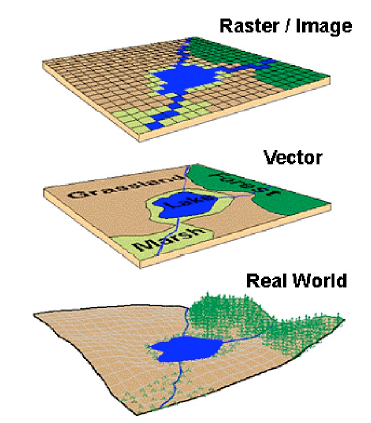
\includegraphics[width=6cm]{Images/Fig_Types_Geodata.png}
    \caption{Vector and raster geographical representation \citep{saabConceptualizingSpaceMapping2003}}
    \label{fig:Fig_data_types}
\end{figure}


% Include image of types of data: Look in \cite{longleyGeographicInformationScience2015} or use image from Andys book

The main use of geographic information is to represent the relative locations of features through a schematic and visual geographic model. With a certain level of abstraction, detail and scale, geographic modelling (mapping) produces knowledge related to the location and the features of the subject of study \citep{longleyGeographicInformationScience2015}. Hence, a geographic information system (GIS), consists of the systematic collection of geo-referenced attribute data. Gifted with powerful processing capabilities, 'GI systems are computer-based tools for collecting, storing, processing, analyzing, and visualizing geographic information' \citep{longleyGeographicInformationScience2015}.

% Geographic model

% enables one to record and represent the location  

% Abstraction and scientific method reference

% Map as a model to represent reality

% Reference to urban modelling for transport

As computing does in most cases, computer-based GIS offers the capacity of processing data in a fraction of the time that would take if is performed manually. Similarly, the generation and capture capacity of location-related attributes has widespread \citep{longleyGeographicInformationScience2015}, as the use of digital means has expanded to support all kinds of services and activities. The conjunctions of these two circumstances are aligned with the future scenario portrayed by \cite{wilsonFutureUrbanModelling2018} with the use of urban modelling covering new unattended spatial modelling and analysis needs.

When leveraging GIS technology to contribute to a specific topic or situation, the use cases vary enormously. As an example of the versatility of GIS to address location-related topics, \citep{longleyGeographicInformationScience2015} listed possible scenarios which include:

\begin{itemize}
\item Impact assessment of possible transport infrastructure.
\item Shipping route planning optimization.
\item Health services coverage.
\item Location intelligence for retailers shore expansion.
\item National parks and natural resources management.
\item Agriculture resources consumption.
\item National defence resources allocation.
\item Tourism navigation and reviewing tools.
\end{itemize}

The geo-processing involved in GIS modelling relies on a wide range of geometrical and mathematical operations. Depending on the type, nature and purpose of the modelling process, different computational procedures are performed to transform the inputs into the intended outcomes that hopefully contribute to the area of study. These methods are usually supported by processing algorithms composed of sequential simpler operations like time, distance, length and area computing. 

% As the GIS derive its operation in  geoprocessing workflows, next some examples of the intermediate results are listed:


% \begin{itemize}
% \item Geometric relations related operations.
% \item Aggregation or dis-aggregation across spatial units.
% \item Spatial and non-spatial data interrelation.
% \item Spatial subsetting.
% \item Proximity analysis.
% \item Time travel matrix computation.
% \end{itemize}

% \begin{itemize}
% \item Point pattern analysis.
% \item Spatial correlation analysis.
% \end{itemize}


In that sense, GIS can be used to address a wide range of location-sensitive topics as they enable and support spatial modelling processes to test future scenarios according to the applicable use case.

PENDING


% Illustrate intermediate results

% Feature management engineering
% Geometry operations
% Geoprocessing
% format conversion
% projection
% Aggregation


% REfenrece to specific GIS measures

\section{Accessibility modelling}

The concept of urban accessibility can be defined as the 'with which people can reach places and opportunities – or, conversely, a characteristic of places and opportunities in terms of how easily they can be reached by the population', \cite{geursAccessibilityEvaluationLanduse2004b} and \cite{neutensEquityUrbanService2010}. Alternatively, \cite{paezMeasuringAccessibilityPositive2012} further expands the definition by framing accessibility into two main components: 'the cost of travel...and the quality/quantity of opportunities'. The cost of travel can be understood as either the monetary cost or the duration or time of the trip to reach the destination, depending on the modelling setup and purpose.

Important to realize that the universal meaning of the word accessibility can represent different concepts. \cite{pereiraIntroductionUrbanAccessibility2023a} presented how accessibility can be understood differently depending on the scale and the context where is applied. On one hand, macro or urban accessibility refers to the effortless ability of people in reaching locations of interest. On the other hand, micro-accessibility is related to how spaces are suitable for people with different levels of mobility or reasoning challenges. 


% Mobility vs accessibility

Likewise, accessibility and mobility are both terms constantly used in the transport assessment context that represent different concepts. Their main distinctive feature can be summarized 
as 'Accessibility,..., refers to the potential ability to reach activities and opportunities. While a mobility analysis would focus, for example, on the time people spend commuting...' \cite{pereiraIntroductionUrbanAccessibility2023a}. Regarding the benefits of introducing the use of accessibility measures in transport planning, \cite{ferreiraAccessibilityGoldMobility2012} argued that planning practitioners should include accessibility measures as it better captures the real benefits in transport-related assessment.

% Reference to other authors in Colombian or non-Colombian cases

From a global perspective, the aggregate results that urban accessibility provides can also be used to measure contributions related to sustainability. As the measure encapsulates the interaction between transport and opportunities, it explicitly relates to sustainability development goal \# 11 'Make cities and human settlements inclusive, safe, resilient and sustainable' \citep{unitednations17GOALSSustainable2015}. Under this sustainability development goal (SDG), both topics 'Sustainable transport' and 'Sustainable cities and human settlements' are aligned with the use of accessibility measurements, considering that it quantitatively captures the principles that these topics promote.

Regarding the interpretation and use of an accessibility-based measure, there are references in the urban development field.  

\cite{pereiraIntroductionUrbanAccessibility2023a} highlighted how it manages to holistically capture the overall result of the transportation offer, the distribution of strategically important activities and the location of individuals within the study area. Additionally, \cite{pereiraIntroductionUrbanAccessibility2023a} stated how accessibility is also related to social inclusion as it accounts for not only the current functioning transport system but also how this system allows individuals to access the location of their interest.

\cite{papaAccessibilityInstrumentsPlanning2016} and \cite{boisjolyHowGetThere2017} stated how accessibility measures are used in transport assessment contexts. \cite{boisjolyHowGetThere2017} presented how accessibility measures favour a more systematic assessment of transportation needs being covered, although their use has not been widespread among transport planning practitioners as the authors expected. \cite{boisjolyHowGetThere2017} considered transport plans from cities in Europe, North America, Australia and Asia.
In contrast, \cite{papaAccessibilityInstrumentsPlanning2016} showcased several European examples where accessibility measures were included in the assessment considered in routine planning practices.

% Brief explanation of accessibility measures

Within accessibility, multiple measures are available to model how easily people can reach their destinations of interest. \cite{paezMeasuringAccessibilityPositive2012} and \cite{dijstOpportunitiesTransportMode2002}, presented a general review of the main groups of accessibility measures, which are summarized and listed next:

\begin{itemize}
  \item Place-based measures: The place-based measures aim to quantity the ability to reach opportunities from a specific location in space due to the spatial distribution of opportunities and the transport network available. These measures can be grouped as follows:
    \begin{itemize}
        \item Cumulative opportunity measures: The cumulative measure considers the total of opportunities that can be reached from a given location that complies with a time or travel cost threshold.
            \begin{itemize}
                \item Active cumulative accessibility measure: It consists of the number of opportunities that a person located in a given location can access with ease within a threshold. 
                \item Passive cumulative accessibility measure: It reflects the number of people that can reach a certain destination or opportunity without exceeding the travel cost threshold.
            \end{itemize}
        \item Minimum travel cost: It maps the nearest locations of interest (opportunity) by considering the one destination with the lowest travel cost, either time or monetary cost.
        \item Gravity measures: Based on Newton's gravitational model, it accounts for variation in travel cost as the distance between the origin and destination location increases.
        \item Floating catchment area competition: The catchment area measure aims to account for the interaction between the offer of opportunities and the demand of individuals according to their spatial distribution and accessibility levels.
        
    \end{itemize}
  \item Person-based measures: In conjunction with the transport network and spatial opportunity distribution, this measure also considers the personal features of individuals in a given location in space.
\end{itemize}

% References to research



% \begin{itemize}
%   \item Success cases of the use of accessibility measures
%   \item Reference to initiatives and efforts from NGO organizations related to urban accessibility: IBD, World Bank, GIZ.
%   \item Reference to north and global south previous research
% \end{itemize}

\section{Colombia and the Bogot\'{a} study case}

In the urban development field, there is an extended list of references related to the use of accessibility applied to transport assessments context. Particular interest in research activities has been expended on areas that have experienced migration and/or relatively more rapid urbanisation processes \citep{kojimaIntroductionPopulationMigration1996}. Latin america and Colombia are not excluded from this trend as the rapid urbanization reinforces the already present inequalities in cities \citep{wrightwendelAccessibilityUsabilityGreen2012,tellezUrbanDevelopmentBogota2018}.


Colombia's capital, Bogot\'{a} has been an area of study of multiple transport and accessibility-related research exercises. That should not come as a surprise considering the population growth that Bogot\'{a} and her surrounding municipalities have experienced over the last couple of decades. By 2017, Bogot\'{a} had almost doubled its population during the last 30 years and similarly did the near municipalities by increasing their population by almost 3 times during the same time period \citep{guzmanCityProfileBogota2017}.

A milestone in Bogotá's transportation history was the operation start of its current BRT 'Transmilenio' system by the beginning of the 21st century \citep{rodriguezValueAccessibilityBogota2004}. Derived from the deployment and the integration of collective bus services in Bogotá, the resulting accessibility effect of the BRT system has been a popular element of study among transport and development-related researchers. The next paragraph intends to explore the previous research exercises that have expanded on the topic of interest of the present research. However, there are clearly other valuable contributions that could not be included due to practical limitations.

% It is clear that the BRT system provided the city with a functioning solution to integrate most of the collective bus services.

Although it was not a proper accessibility assessment as defined in previous sections, \cite{rodriguezValueAccessibilityBogota2004} initially examined the relationship between proximity and land value and found that apparently there was a positive relation between the land price and the proximity to the BRT system stations. However, the influence might be underscored by the short time frame (2 years) between the measure and the operation kick-off of the BRT system.

With a more straightforward social-inequality and accessibility approach, \cite{bocarejos.TransportAccessibilitySocial2012} performed an urban accessibility assessment on the city's BRT system. Considering that their main research goal was to generate an 'analysis tool that helps quantify and differentiate access inequalities' \cite{bocarejos.TransportAccessibilitySocial2012} highlighted the value of introducing the accessibility concept as part of the analysis. Additionally, the authors also considered economic individual constraints that the users might have in order to 'consider not only an indicator that relates the transport system to land use, but the real possibility of transport use and ease of access to the city opportunities depending on individual purchasing power' \cite{bocarejos.TransportAccessibilitySocial2012}.

In a further exercise, \cite{bocarejoAccessibilityAnalysisIntegrated2014} expanded on the accessibility assessment by including additional variables related to the use and related benefit of the BRT system in Bogotá. As the BRT system progressively expanded and integrated more auxiliary routes intended to feed the main corridors of the system, their research purpose was to assess the impact of the integration in accessibility terms. As the integration of the auxiliary routes with the main BRT network was a novel situation at the time, \cite{bocarejoAccessibilityAnalysisIntegrated2014} included further variables in the assessment like the purchasing power of the users and cost/benefit ratio considering multiple possible fare schemes. The results confirmed the relevance of the use of accessibility measures as they found that the integration in fact generated time reductions in the periphery areas of the city, however, affordability constraints can materialize in low-income users \citep{bocarejoAccessibilityAnalysisIntegrated2014}.

Similarly, with a social and equality accessibility approach, \cite{guzmanAssessingEquityTransport2017} performed an accessibility assessment on at a more regional scale. Not only considering Bogotá capital district municipality, \cite{guzmanAssessingEquityTransport2017} included the surrounding municipalities in order to have a more regional-cohesive result. Additionally, privately owned cars, ordinary buses and BRT transportation modes were disaggregated to assess accessibility individually. In terms of the opportunities, that means the destination of interest,\cite{guzmanAssessingEquityTransport2017} particularly focused on jobs and education-related points of interest.

Subsequently, \cite{guzmanAccessibilityAffordabilityEquity2018} carried out a transport accessibility assessment which considered multiple fare subsidy scenarios. By formulating a possible fare subsidy scheme, \cite{guzmanAccessibilityAffordabilityEquity2018} spatially modelled the effect in affordability and accessibility derived from the use of the public transportation network.

% Reference the use of accesibility measures when the transport system is expanding, when a fare is changing, to access impact across different population groups of interest, etc

% \begin{itemize}
%   \item Reference to National (Colombia) and local government (Bogota) plans related to transport infrastructure (or in Chapter 3?)
%   \item SGG in National development plan of Colombia
%   \item Reference to research done in Bogota (or in Chapter 3?)
% \end{itemize}

\chapter{Data} \label{Chap3}

% \begin{itemize}
%   \item Brief context of Bogot\'{a} as Colombia\textquotesingle s capital
%   \item Current Bogot\'{a}\textquotesingle s spatial structure
%   \item Social and spatial population distribution
% \end{itemize}

\section{Summary}

Considering the main components that influence the accessibility measures \citep{pereiraIntroductionUrbanAccessibility2023a}, Table \ref{tab:Data_summary} groups the primary input used to develop the present research project, respectively, while indicating the source in each case.

\begin{table}[H]
\centering
\renewcommand{\arraystretch}{1.6} % Adjust the row height
\resizebox{\textwidth}{!}{%
\begin{tabular}{llll}
\hline
\multicolumn{1}{c}{\textbf{Component}} &
  \multicolumn{1}{c}{\textbf{Input}} &
  \multicolumn{1}{c}{\textbf{Description}} &
  \multicolumn{1}{c}{\textbf{Source}} \\ \hline
\multirow{3}{*}{\begin{tabular}[c]{@{}l@{}}Transport \\ infrastructure\end{tabular}} &
  BRT system &
  Static transit information of current system &
  \cite{transmilenios.a.GTFSEstaticos202306212023} \\
             & Road and walking network & Street network                         & \cite{openstreetmapcontributorsPlanetDumpRetrieved2023} \\
             & Metro system             & Track and station data of future metro & \cite{alcaldiadebogotad.c.TrazadoPrimeraLinea2022,alcaldiadebogotad.c.EstacionesPrimeraLinea2022} \\ \hline
Land use     & Predominant land use     & Predominant use terrain level data     & \cite{alcaldiadebogotad.c.DestinoEconomicoPredominante2022} \\ \hline
Demographics & Multipurpose survey      & Anonymized survey data                 & \cite{secretariadistritaldeplaneacionMicrodatosEncuestaMultiproposito2023,secretariadistritaldeplaneacionCapaGeograficaEncuesta2023} \\ \hline
\end{tabular}}
\caption{Input data summary.}
\label{tab:Data_summary}
\end{table}

The local government of Bogotá (Alcaldia de Bogotá D.C.) generated, directly or indirectly, most of the input information used to model accessibility. The transport infrastructure component groups the data that describes the current and future transportation network of Bogotá. In the case of the transit data used to model the operation of the current BRT network, it was generated and published by Transmilenio S.A., which is a publicly owned company in charge of managing and coordinating the BRT system operation \citep{transmilenios.a.HistoriaTransmilenioHistory2013}. Regarding the Multipurpose Survey information in the demographic component, it was jointly gathered by the Planning Department of Bogotá City Council (Sectretaría Distrital de Planeación) and the National Administrative Statistics Department (Departamento Administrativo Nacional de Estadística - DANE).


The following sections contain a general description of each input data used to model accessibility.





\section{Transport infrastructure}

\subsection{BRT network}

The transit information from the current BRT network systematically both the infrastructure and the transport operation. As the entity responsible for managing the operation of the BRT system, Transmilenio S.A. has published\footnote{Transit information dated 21/06/2023} their transit using a GTFS\footnote{GTFS: General transport feed specification} format. The GTFS format is an open-source standardized format that describes transport operations' main features. Numerous transport agencies are currently using this format as it integrates spatial data, fleet, fare and timetables \citep{pereiraIntroductionUrbanAccessibility2023a, mobiltydataGeneralTransitFeed2023}.

GTFS data comprises tables containing spatial and non-spatial features of the transportation system. Through key fields to trace relationships between the multiple tables, GTFS characterises multimode systems, their routes, fares, frequencies, and timetables, among other features. For example, Figure \ref{fig:GTFS_structure} illustrates the general structure of GTFS data and how the tables relate. Similarly, Table \ref{tab:GTFS_description}, describes the main features of every table in the GTFS data structure.

Important to note the relation between route and trip information in the GTFS data structure, presented in \ref{tab:GTFS_description}. The route table indicates the routes that compose the transport system. In a similar matter but at a lower transport system hierarchy level, trips should be understood as transport service units comprising each route \citep{pereiraIntroductionUrbanAccessibility2023a}. In other words, the trip service units are how the transport operation of each route materializes.

\begin{figure}[H]
    \centering
    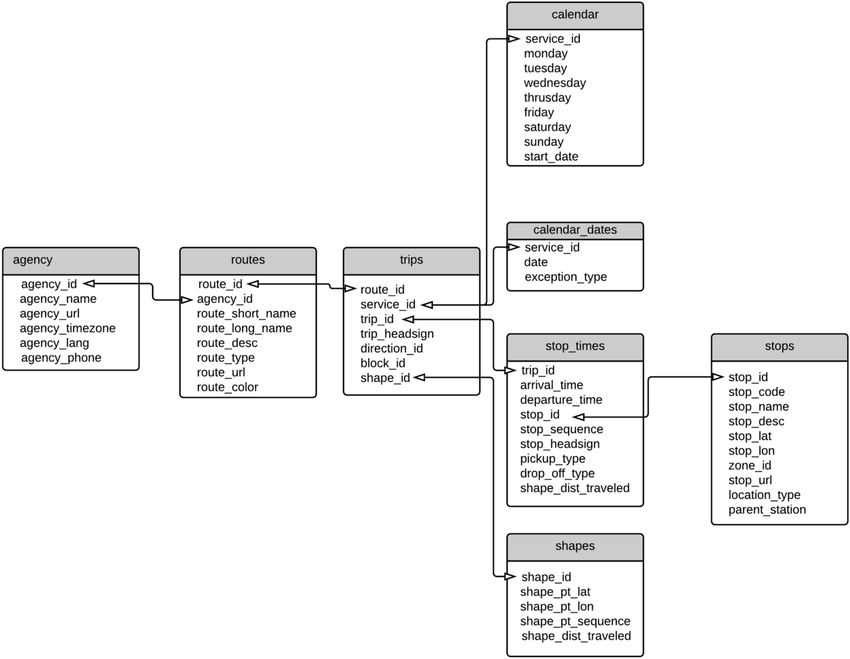
\includegraphics[width=10cm]{Images/GTFS-data-format.png}
    \caption{GTFS data structure (\cite{pereiraExploringTimeGeography2023} cited by \cite{pereiraIntroductionUrbanAccessibility2023a})}
    \label{fig:GTFS_structure}
\end{figure}

\begin{table}[htp]
\centering
\renewcommand{\arraystretch}{1.5} % Adjust the row height
\resizebox{\textwidth}{!}{%
\begin{tabular}{lll}
\hline
\multicolumn{1}{c}{\textbf{Table name}} & \multicolumn{1}{c}{\textbf{Topic}} & \multicolumn{1}{c}{\textbf{Description}}                  \\ \hline
agency                                  & Transport providers                & General transport providers data including transport mode \\ \hline
routes          & Routes information        & Transit routes of the system                     \\ \hline
trips           & Trips information         & Unit of transit service for routes of the system \\ \hline
shapes          & Route geometry            & Route path spatial information                   \\ \hline
stops           & Stations                  & Spatial location of stations                     \\ \hline
stops\_times                            & Trip schedule                      & Arrival and departure time of trips in each station       \\ \hline
frequencies     & Frequencies of trips      & Service frequencies of each trip                 \\ \hline
calendar        & General calendar schedule & Weekday general service scheduling               \\ \hline
calendar\_dates                         & Specific calendar schedule         & Special inclusions or exceptions in service scheduling    \\ \hline
fare\_attibutes & Fare description          & General fare conditions                          \\ \hline
fare\_rules     & Fare class description    & Class and fare parameters                        \\ \hline
\end{tabular}}
\caption{GTFS tables general description \citep{mobiltydataGeneralTransitFeed2023}}
\label{tab:GTFS_description}
\end{table}

% map of BRT geometries
Figure \ref{fig:BRT_route_type} shows that Bogotá's BRT network comprises a multilevel route network. Apart from the main corridor BRT network, the system has been expanded into additional complementary routes that are described next:

\begin{itemize}
  \item Main: The route under the main category consists of the exclusive lane routes in the main corridors of the system.
  \item Feeder: The feeder routes are bus routes that use non-exclusive lanes in the road network. Their main role in the system is to connect nearby areas with the main corridors.
  \item Urban: The urban routes offers bus transit services across the city using non-exclusive road lanes.
  \item Complementary and Special: These routes also use non-exclusive lanes from the road network and their grouping category is more related to system operation management.
\end{itemize}

\begin{figure}[H]
    \centering
    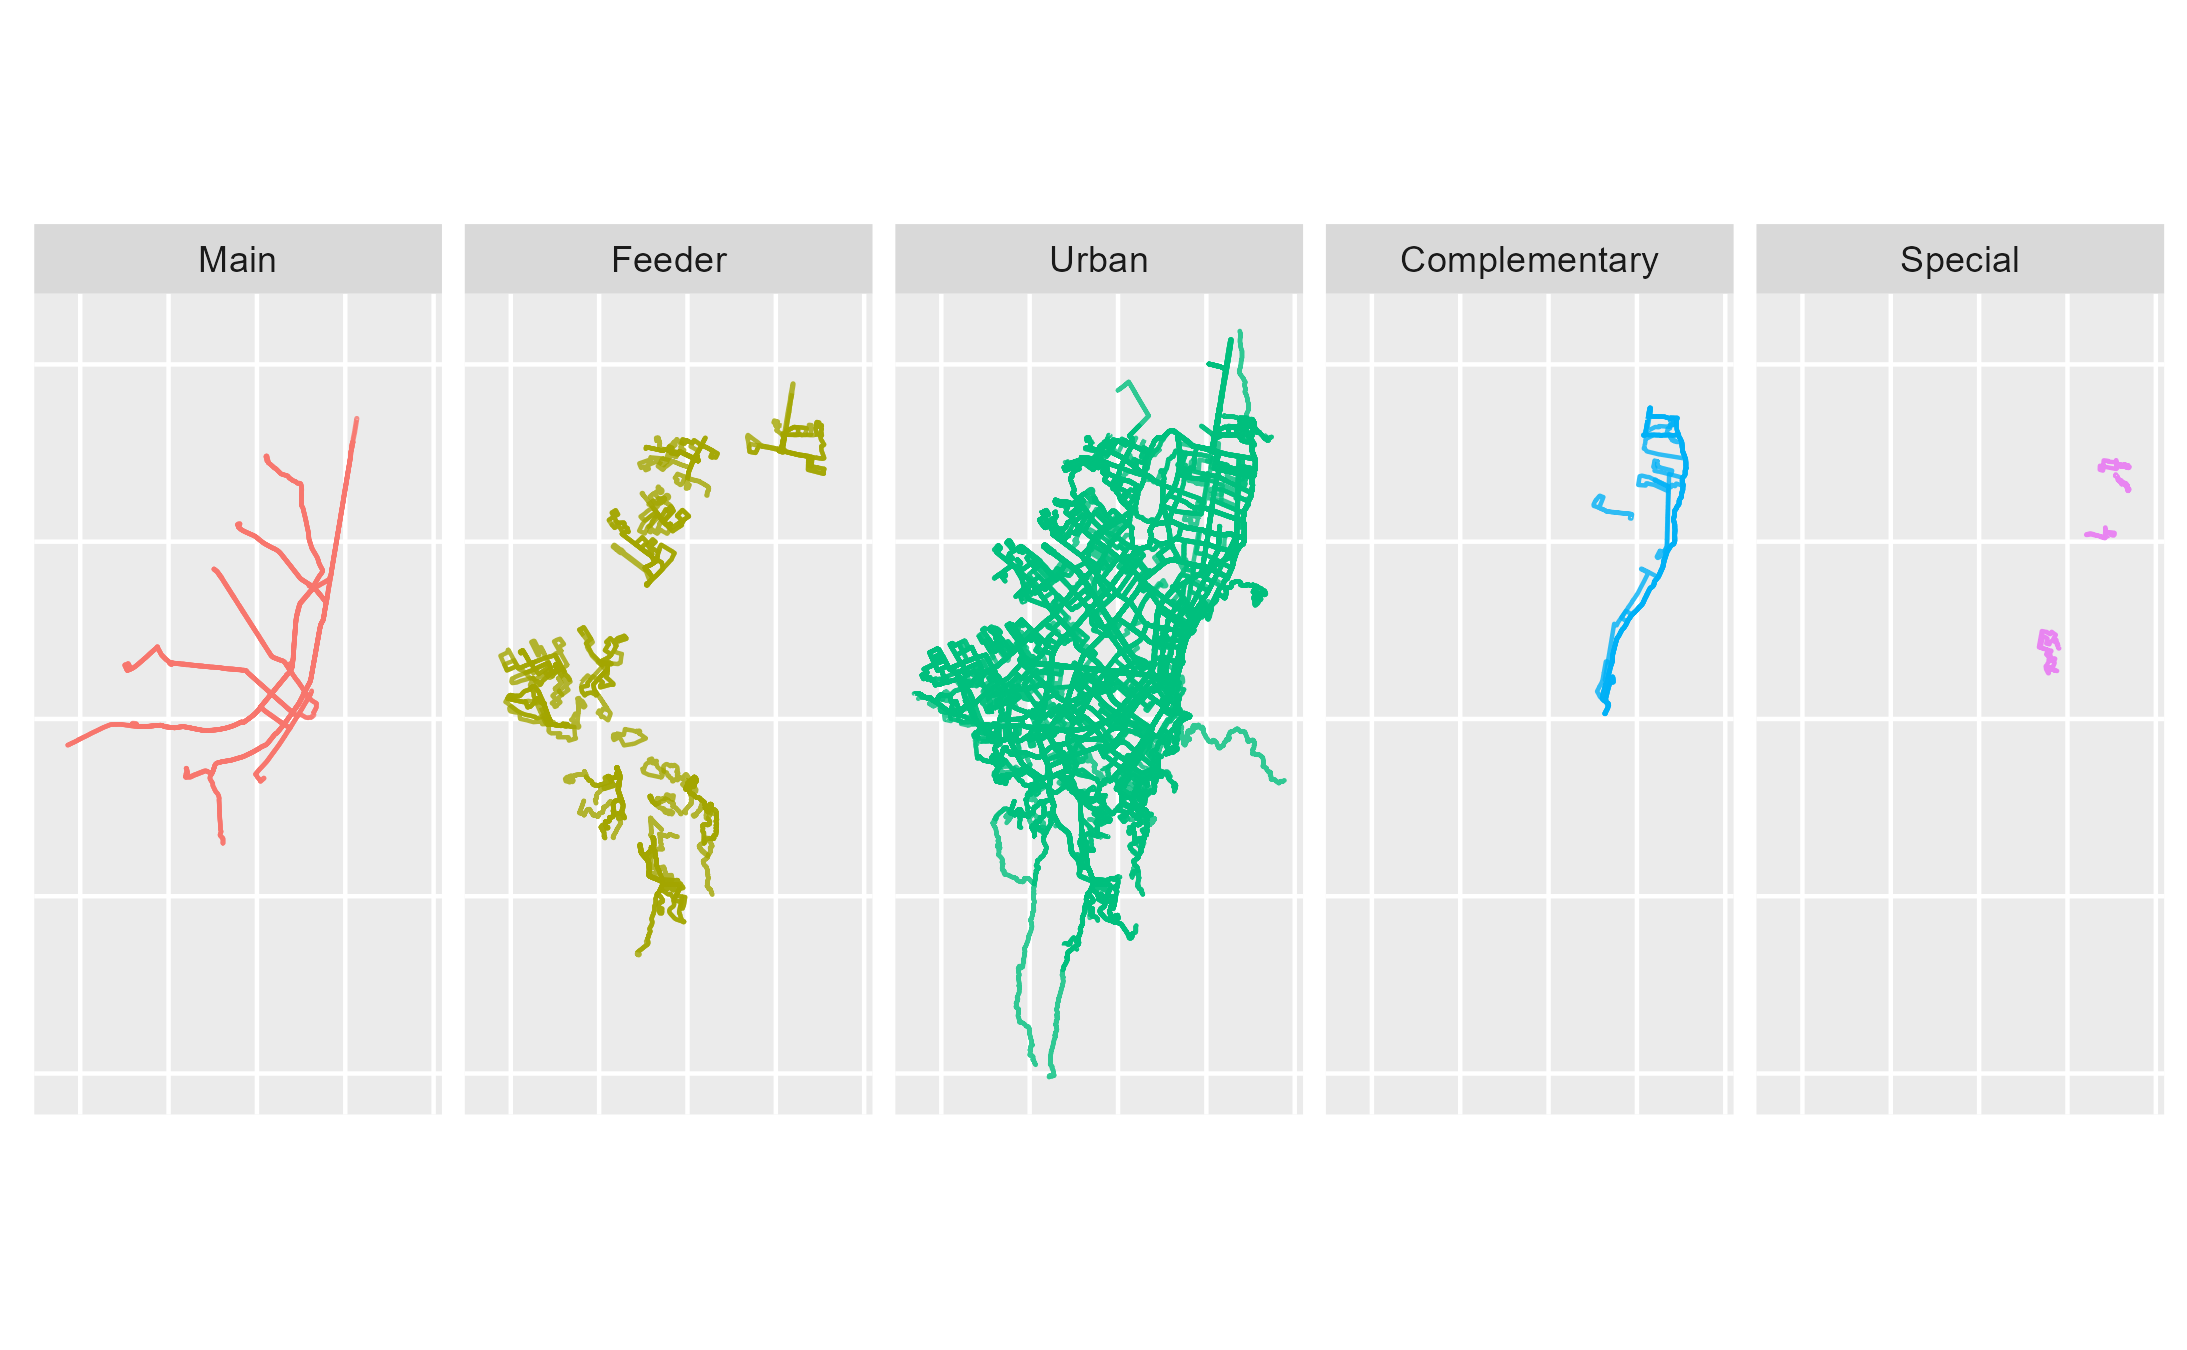
\includegraphics[width=15cm]{Data/Results/Images/BRT_Network_Route.png}
    \caption{BRT network by route type \citep{transmilenios.a.GTFSEstaticos202306212023}}
    \label{fig:BRT_route_type}
\end{figure}

\subsection{Road and walking network}

As commuting practices rely upon more than one mode of transportation, the modelling process requires considering the mode available to reach the desired destinations from the trip's origin. To access a motorized transport mode or make complete mono mode trips, walking constitutes an essential element when modelling commuting trips, therefore, in the accessibility modelling process.

The road and walking network of Bogotá was taken\footnote{Extracted data dated 01/07/2023.} from Open Street Map (OSM) available through \cite{hotexporttoolHOTExportTool2023}. All the transport-related available features were extracted to replicate the possible physical infrastructure for walking. The data format in which the data was downloaded is Protocol Binary Format (PBF), the OSM native vector data format.

\begin{figure}[H]
    \centering
    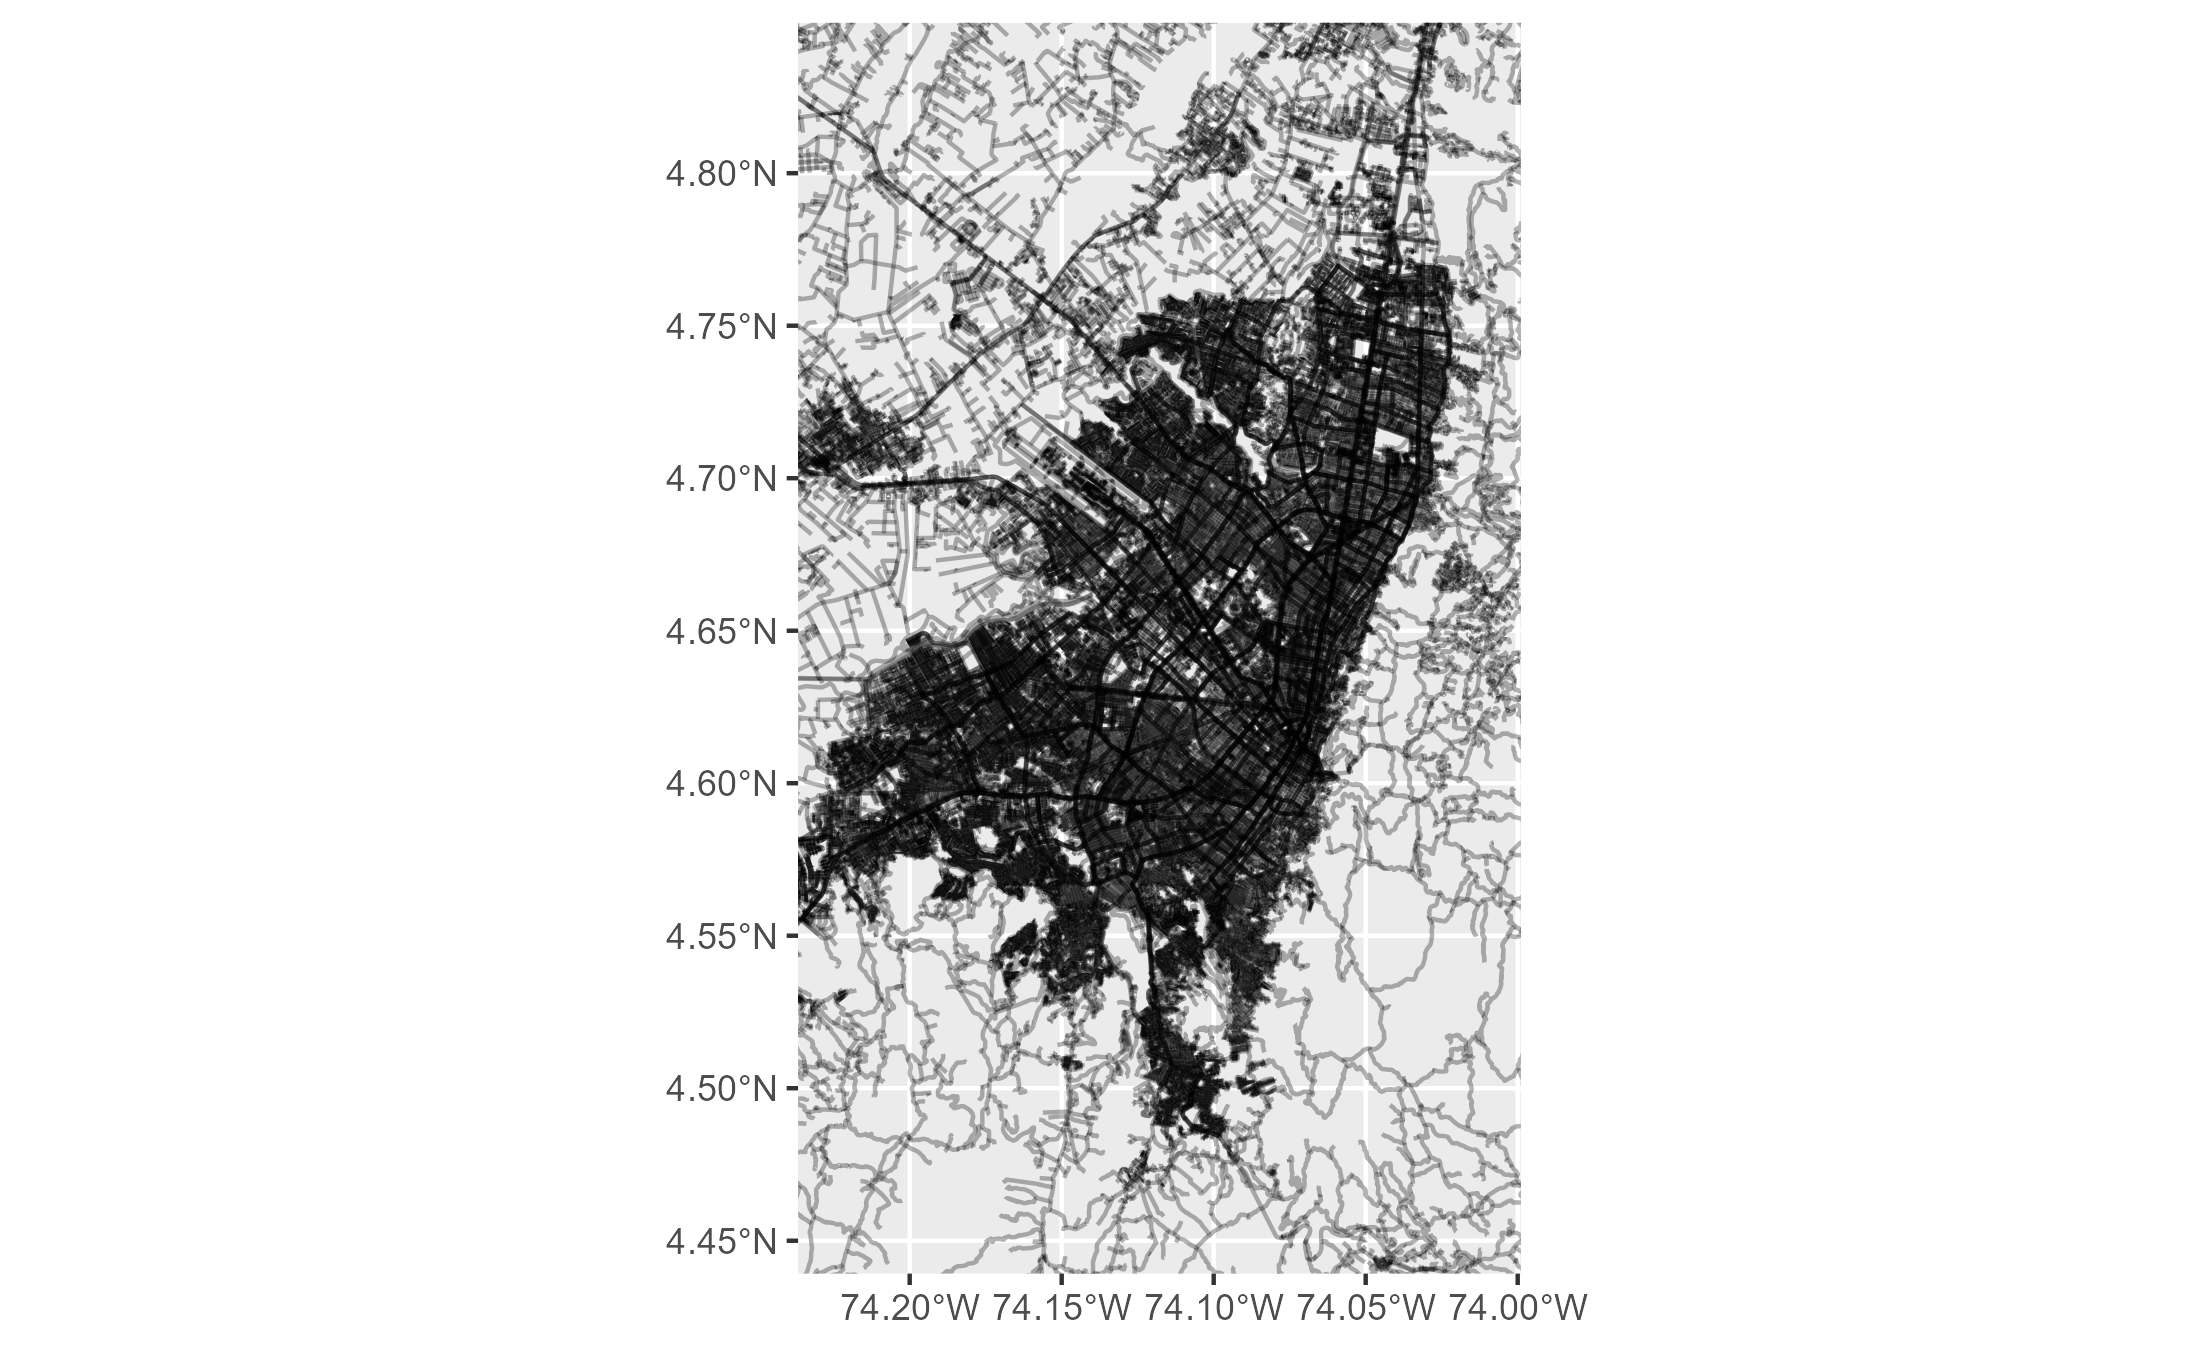
\includegraphics[width=15cm]{Data/Results/Images/OSM_Network.png}
    \caption{Street network infrastructure \citep{openstreetmapcontributorsPlanetDumpRetrieved2023}}
    \label{fig:OSM_Network}
\end{figure}

Figure \ref{fig:OSM_Network} shows an overview of the transport-related infrastructure of Bogotá extracted from OSM. 

% no subsetting
% Closest to reality
% Refence to vector data

\subsection{Metro network}

The metro transport infrastructure data was taken from the publicly available designs of the first line of the future metro. Bogotá city council has published the spatial data related to the main features of the future metro system. The spatial information includes the location of the stations and the geometry track path.

Figure \ref{fig:Metro_Network} presents the track locations, stations, and Bogotá municipal boundary. The 23.9-kilometre length track line follows a north-south direction in the east zone of the city to later connect the east-south and west-south of Bogotá.

\begin{figure}[H]
    \centering
    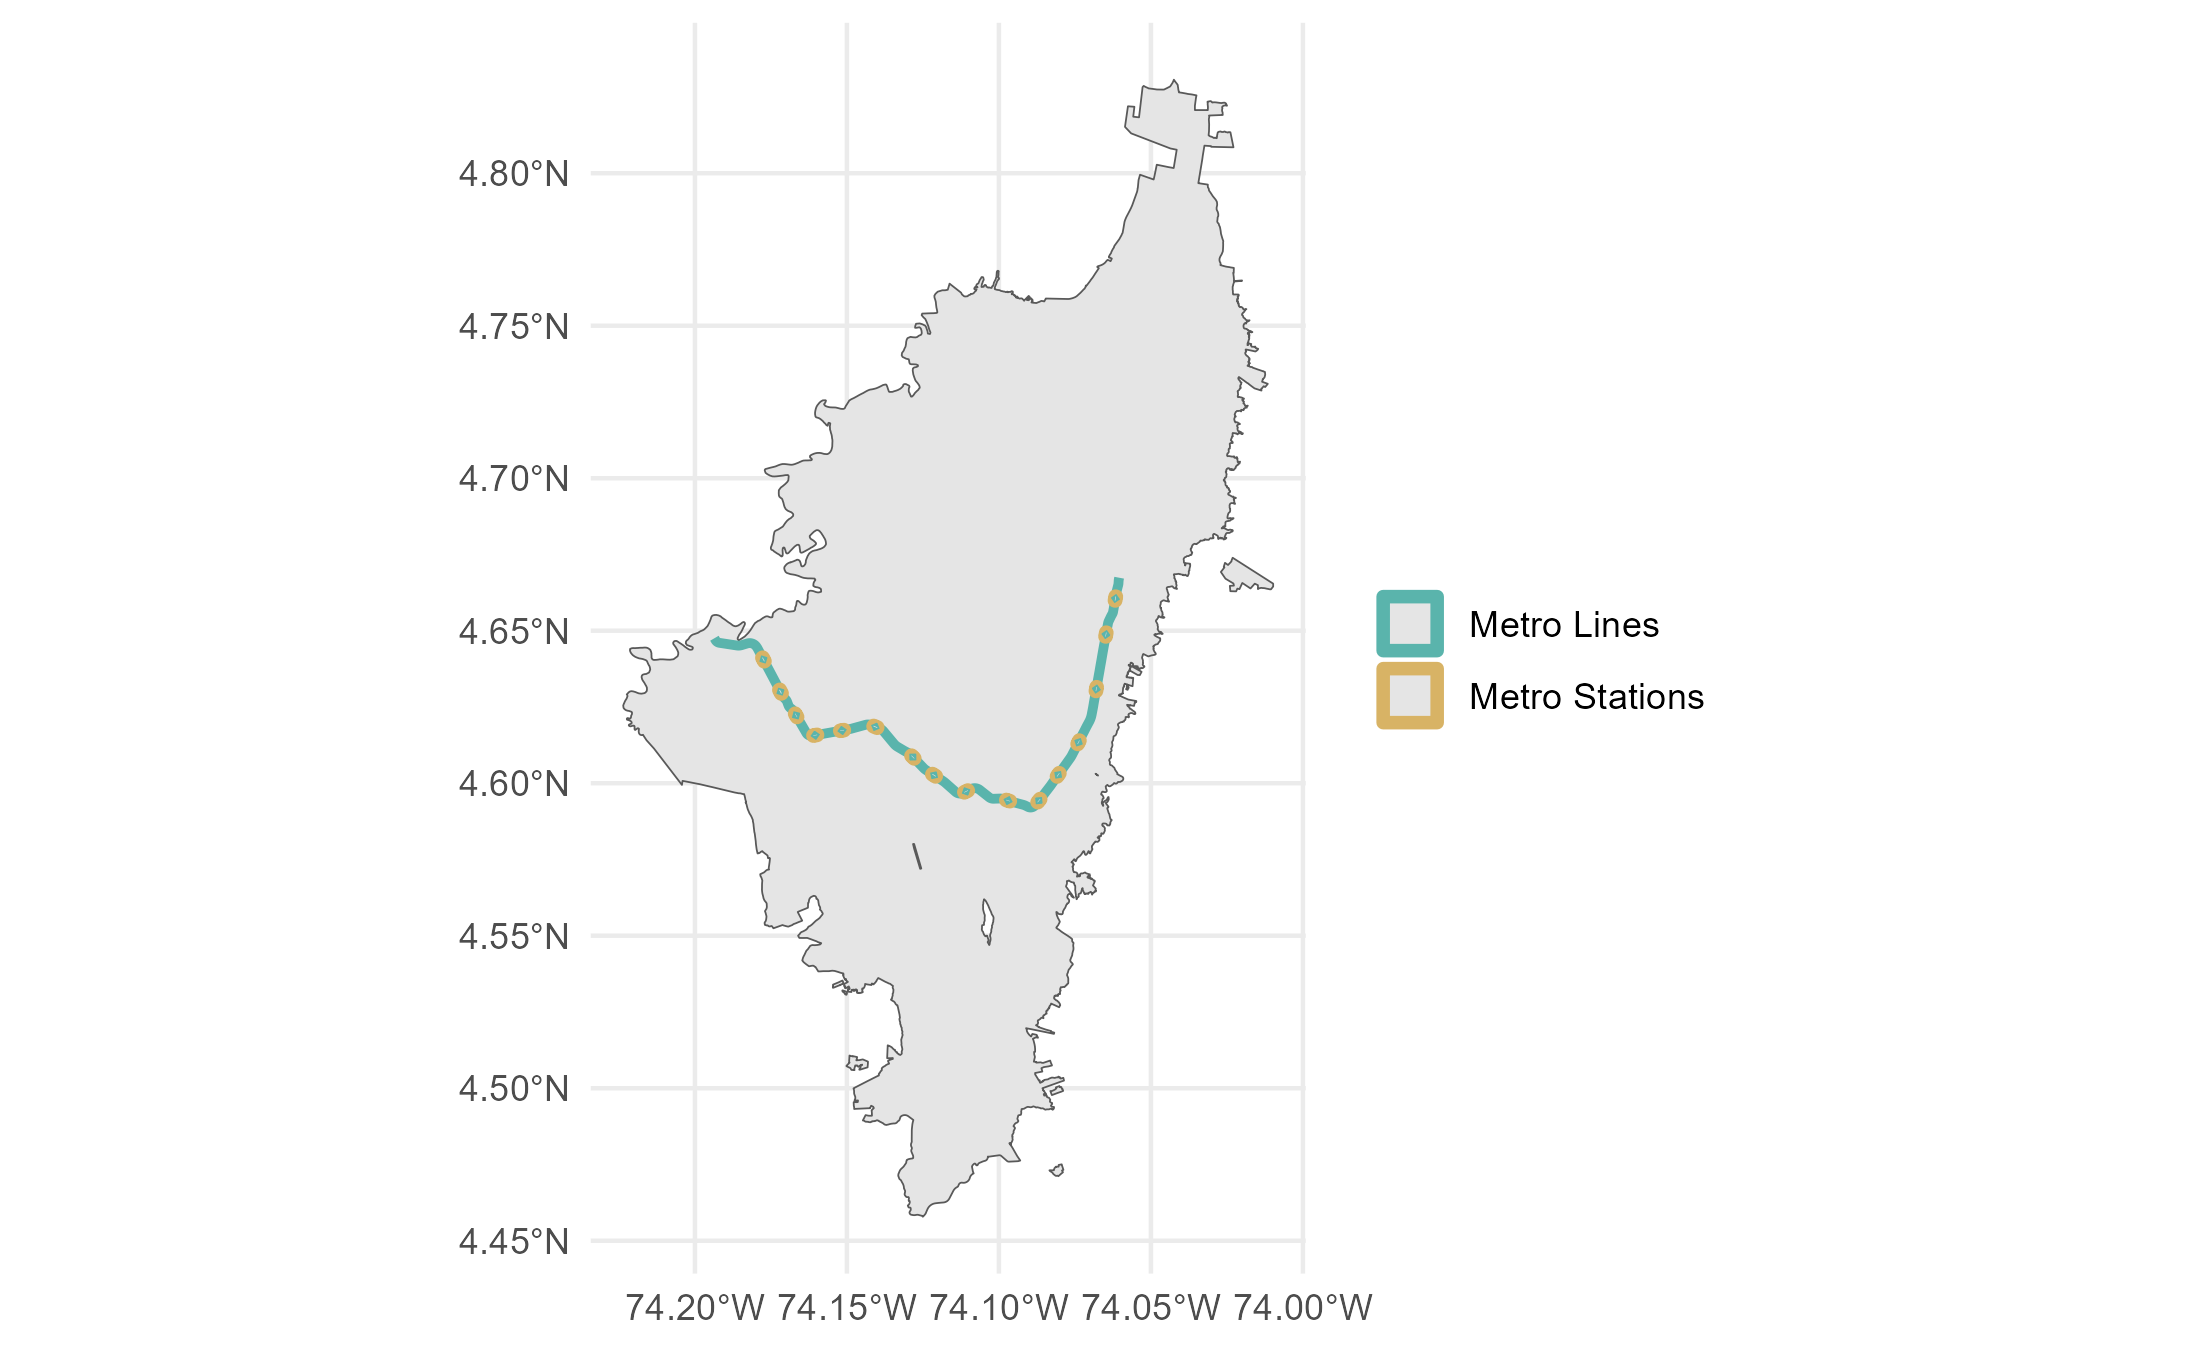
\includegraphics[width=15cm]{Data/Results/Images/Metro_Network.png}
    \caption{Future metro infrastructure \citep{alcaldiadebogotad.c.EstacionesPrimeraLinea2022, alcaldiadebogotad.c.TrazadoPrimeraLinea2022}}
    \label{fig:Metro_Network}
\end{figure}

\section{Land use}

Land use data allows classifying properties according to their predominant economic use. Through terrain spatial data published by \cite{alcaldiadebogotad.c.DestinoEconomicoPredominante2022} it is possible to compute the spatial distribution of properties by their primary land use. Figure \ref{fig:Land_Use_Commercial} shows the spatial distribution of terrains in bogotá classified as commercial corridor land use, with clusters mainly in the east zone of Bogotá. 

\begin{figure}[H]
    \centering
    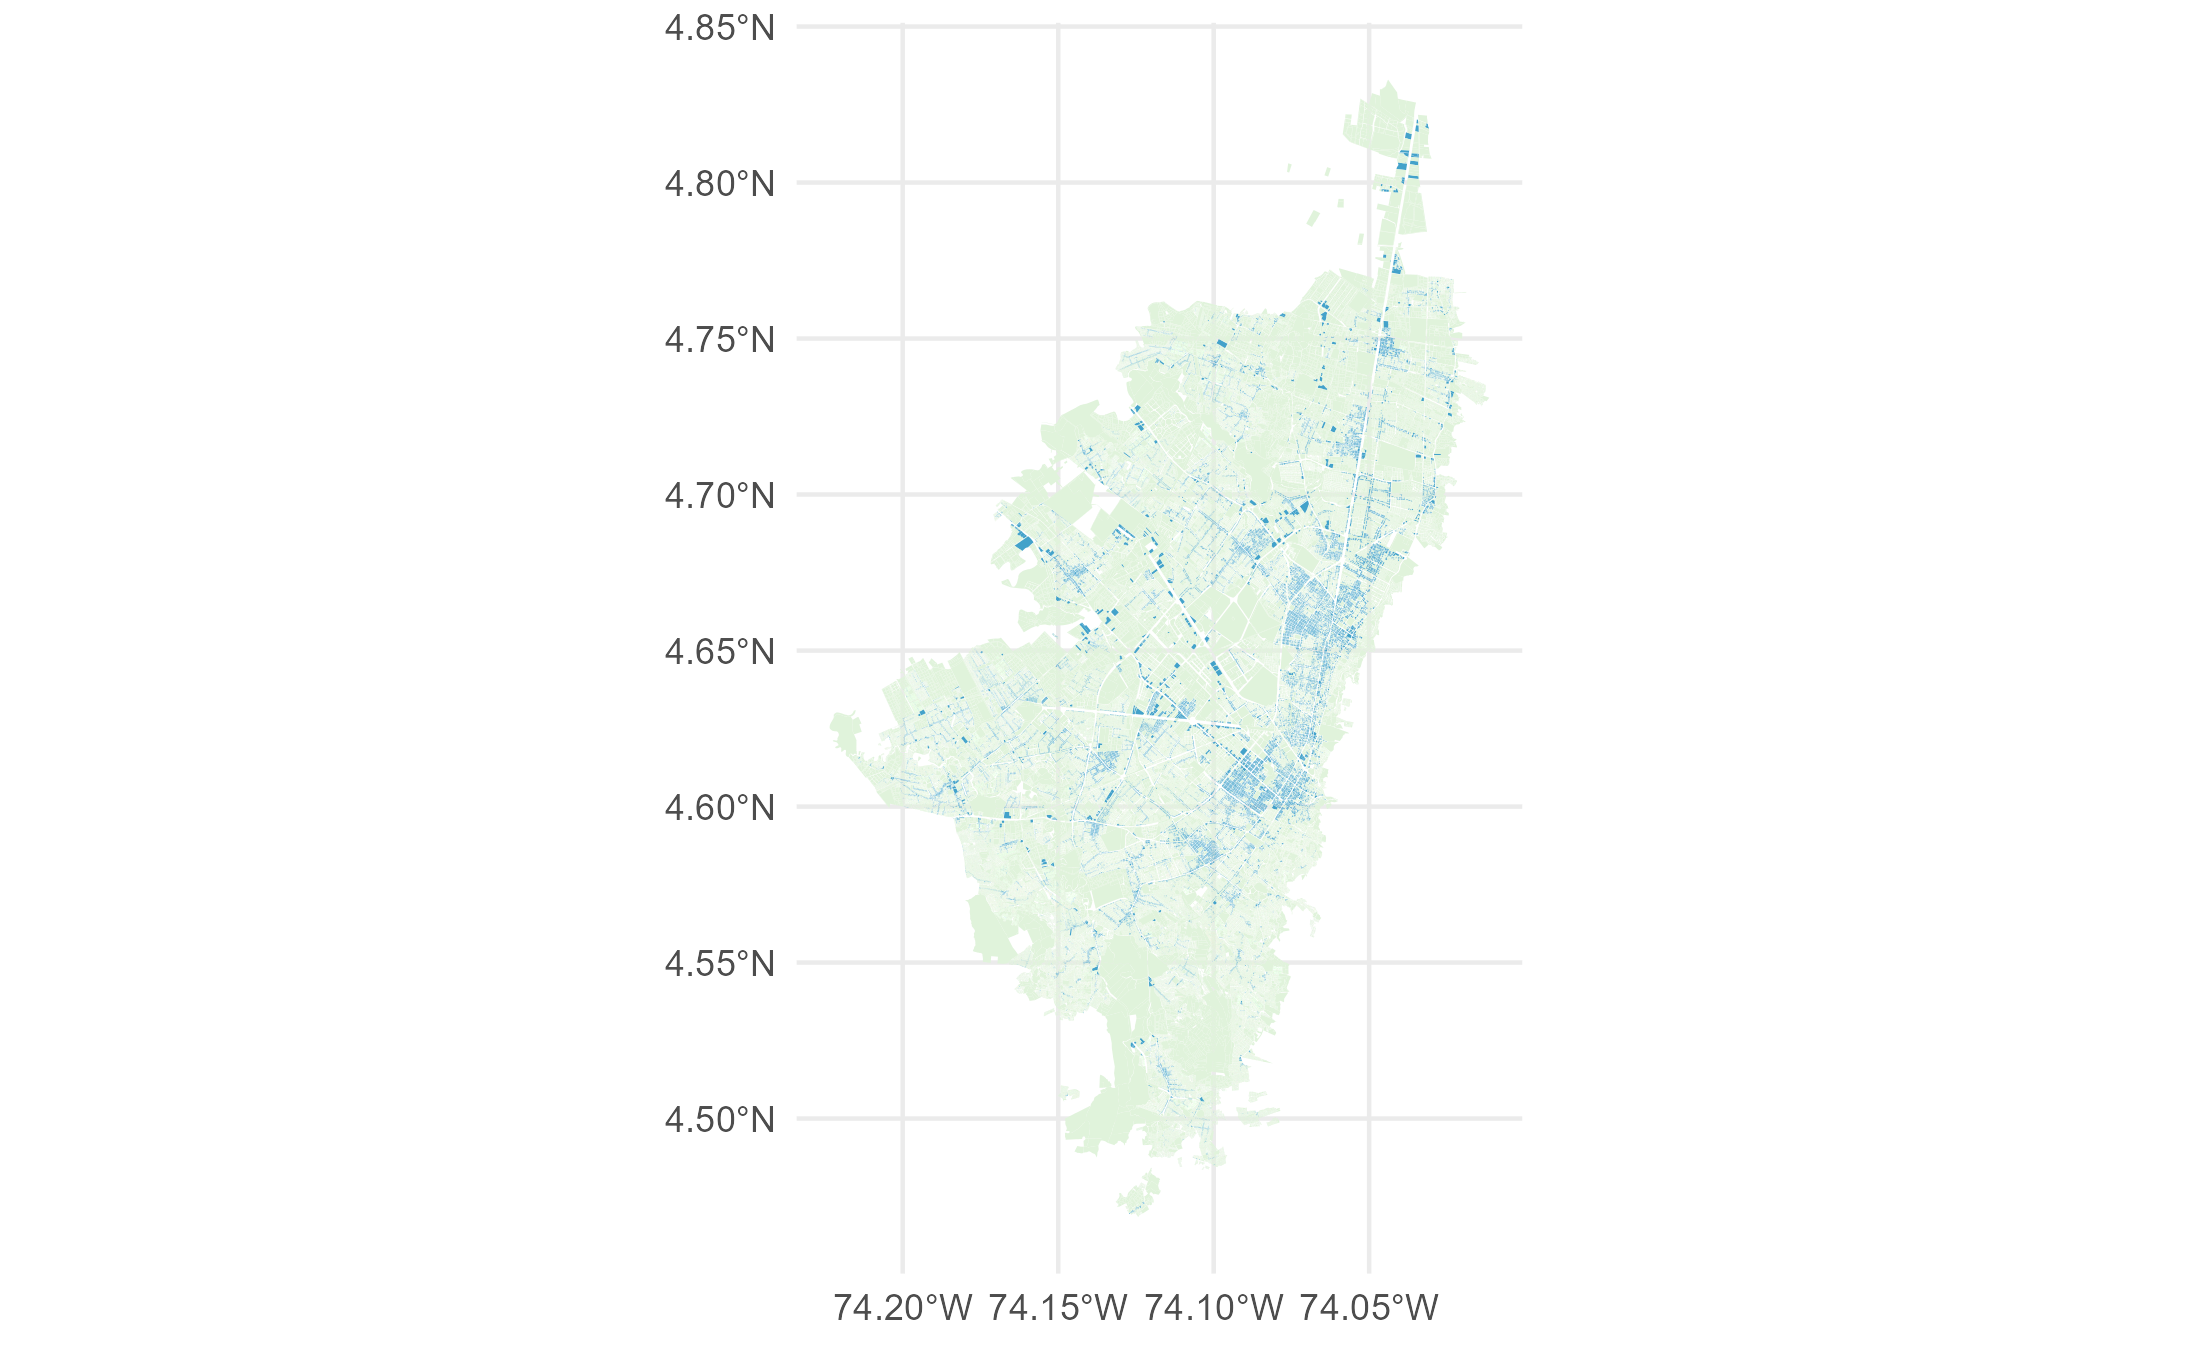
\includegraphics[width=15cm]{Data/Results/Images/Land_Use_Commercial_Corridor_Terrain.png}
    \caption{Terrains with commercial corridor land use \citep{alcaldiadebogotad.c.DestinoEconomicoPredominante2022}}
    \label{fig:Land_Use_Commercial}
\end{figure}

\section{Demographics}

% Reference to the survey
% Reference to the GIS layer

With a multipurpose approach, \cite{secretariadistritaldeplaneacionCapaGeograficaEncuesta2023} gathered information through a survey from Bogotá's households. The multipurpose survey captured multiple variables at a residential, household and personal level of Bogotá's population. Among the topics covered in the survey, it included variables related to living conditions, housing, utilities, health, education and demographics.

The survey data has been gone through an anonymization procedure done by \cite{secretariadistritaldeplaneacionMicrodatosEncuestaMultiproposito2023} to keep non-spatial and spatial attributes unexposed. The residential location of the public surveyed is not published. However, the data can be spatially aggregated by the zoning planning unit (ZPU) used by Bogotá City Council as a spatial-administrative subdivision of their main boroughs. As the survey microdata contains the corresponding ZPU where each survey was collected, it is possible to aggregate the results spatially. 

Figure \ref{fig:Demo_Income_ZPU} present the median household income by ZPU in Bogotá. The highest median income values are registered in the northeast part of the city, while the lowest are found in the south and southwest area.

\begin{figure}[H]
    \centering
    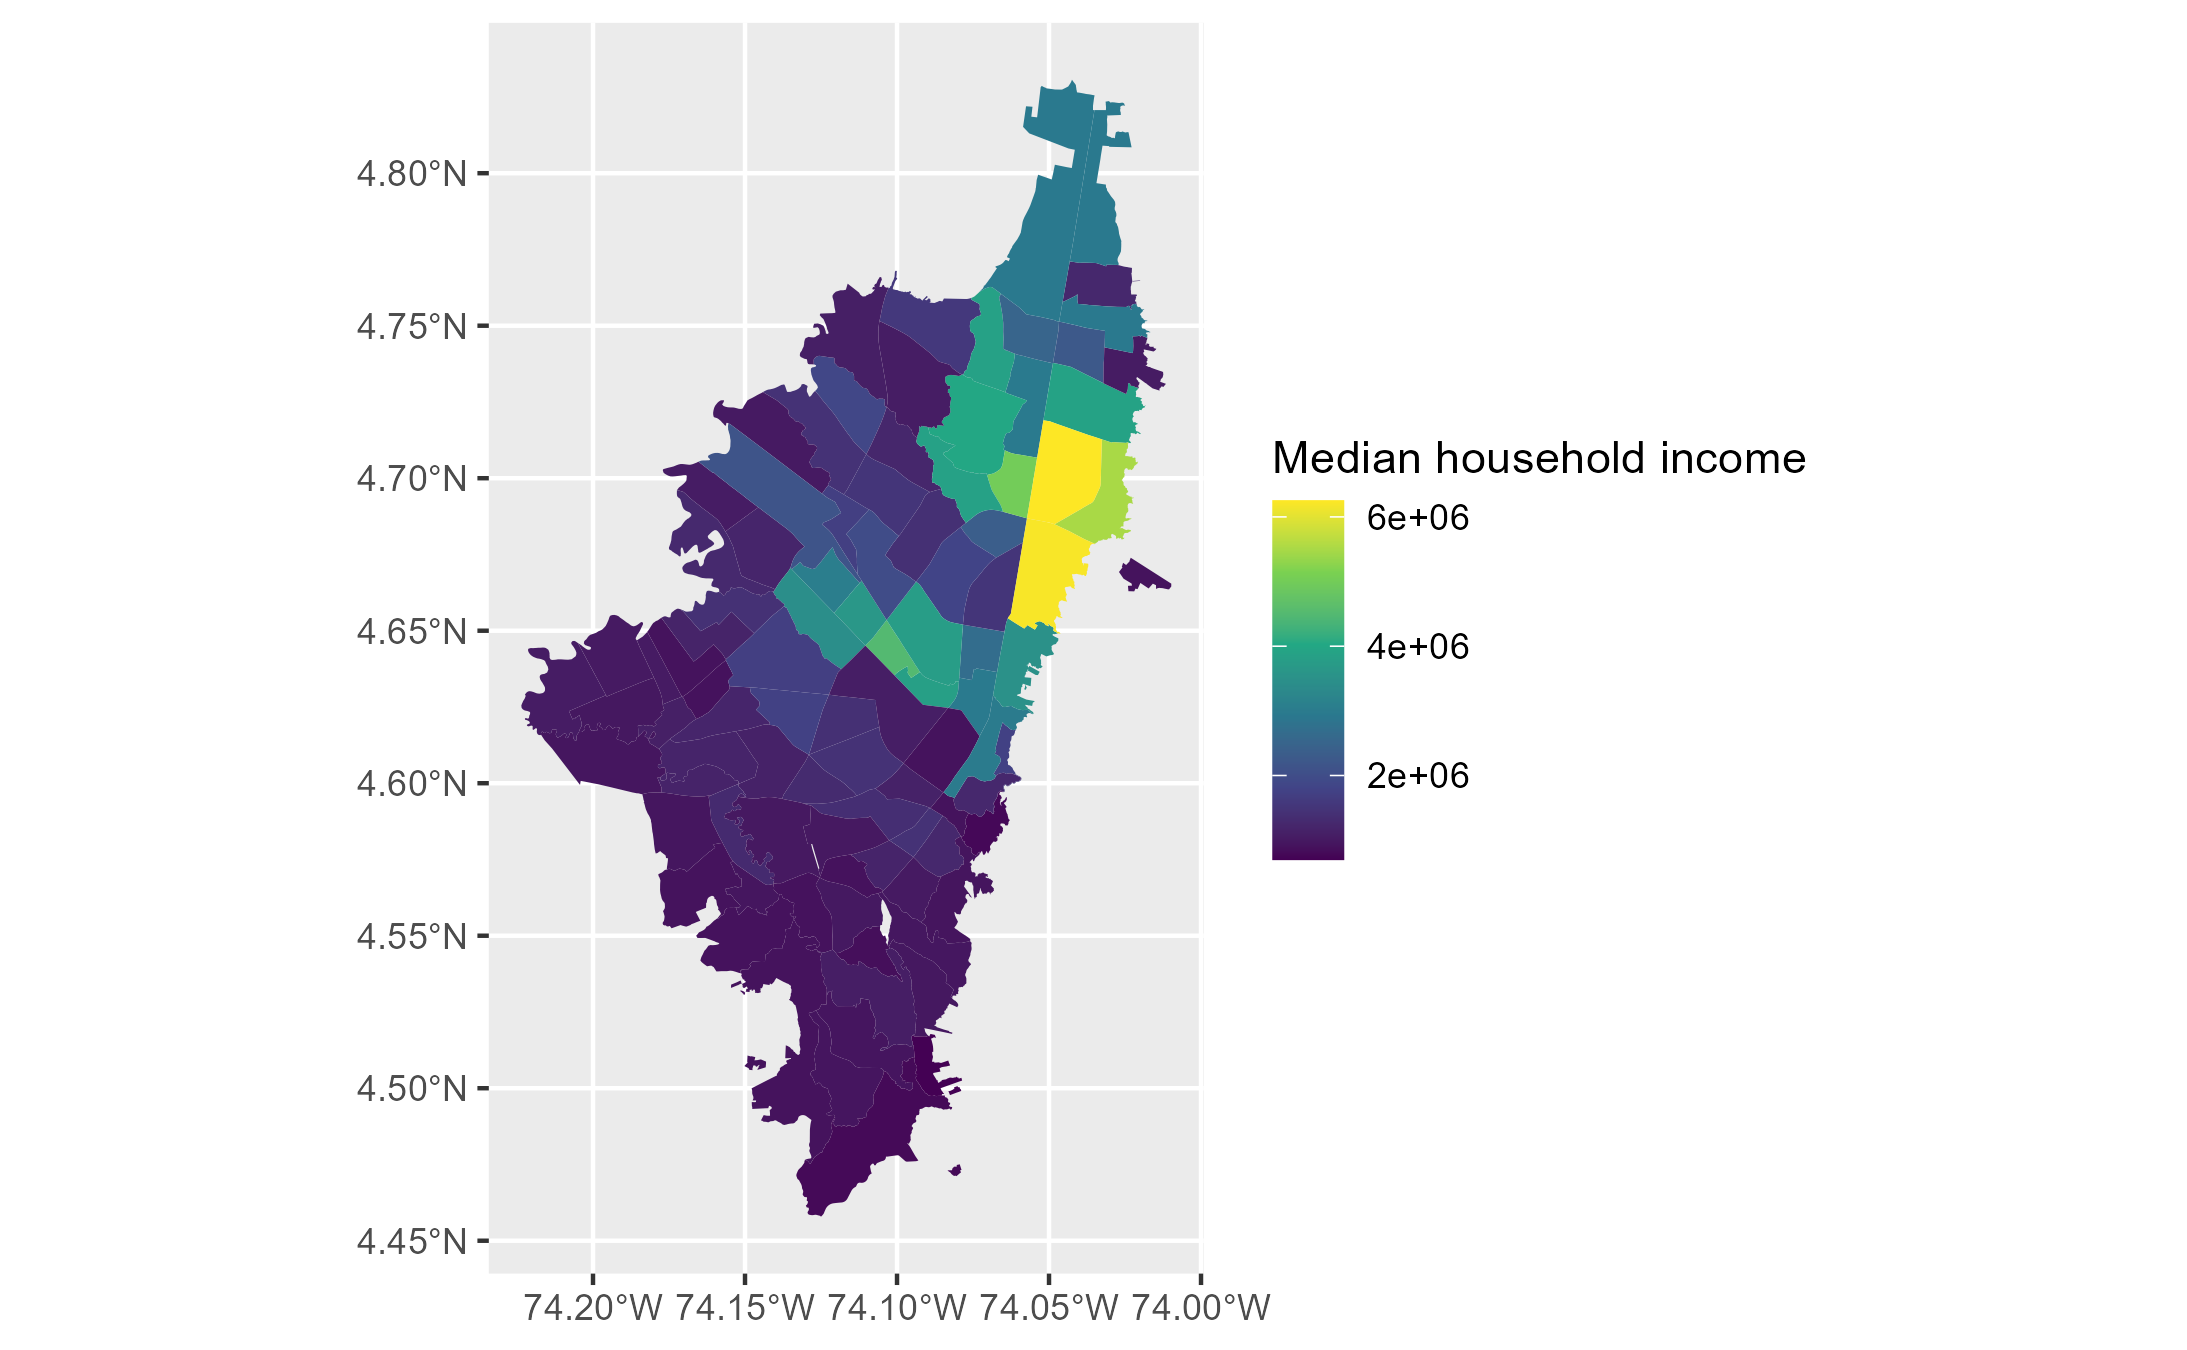
\includegraphics[width=15cm]{Data/Results/Images/Demo_Income_UPZ_Mean_Median.png}
    \caption{Median household income by Zoning Planning Units (ZPU) \citep{secretariadistritaldeplaneacionMicrodatosEncuestaMultiproposito2023, secretariadistritaldeplaneacionCapaGeograficaEncuesta2023} }
    \label{fig:Demo_Income_ZPU}
\end{figure}


\chapter{Methodology} \label{Chap4}


\section{Overview}

The literature explored above presents an overview of how urban modelling enables future scenario assessment that can reorient transport-related planning practices by introducing accessibility measures. Strictly mobility-based transport policymaking practices can fall short of fully assessing the real tangible benefits of transport infrastructure projects. Additionally, inhabitants' spatial distribution and socioeconomic conditions can differ dramatically within the urban context. As a result, the accessibility measurement result denotes a different level of deprivation and urgency outlook depending on the living conditions identified in the location of interest. Therefore, apart from introducing accessibility-based measures when assessing transport infrastructure projects, the results should be disaggregated into population groups of interest who might be experiencing the most precarious living conditions. For this reason, prioritizing relative accessibility improvements across population groups experiencing a higher degree of deprivation or vulnerability should be considered when promoting any transport-related initiative.


Hence, this study measured urban accessibility for the current and future metro scenario in Bogotá, Colombia. Using a before and after comparison analysis, this research calculated the accessibility improvement derived from the future transit operation of Bogotá's metro system, combined with the current functioning BRT network.

\begin{figure}[H]
    \centering
    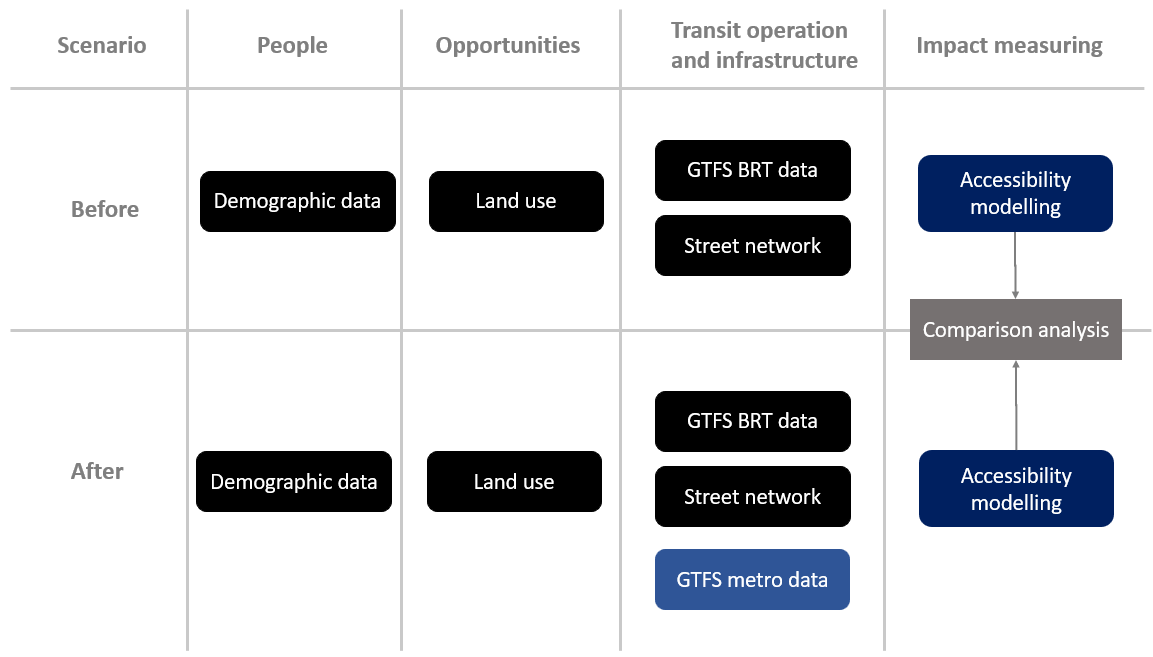
\includegraphics[width=16cm]{Images/Method_Summary.png}
    \caption{Method summary diagram}
    \label{fig:Method_Summary}
\end{figure}

First, this study generated projected transit data for the metro system based on the main features and spatial data already published by Bogotá's local authorities. Second, land use and demographic data are integrated into a spatial framework to track the spatial distribution of economic activity and to assess living conditions in Bogotá's inhabitants spatially. Finally, by integrating transit information from before and after scenarios, the study maps how the accessibility levels will spatially vary by population groups of interest with the construction and operation of the new metro system. The analysis, preprocessing, modelling and visualization process was conducted using R Programming Language. For the accessibility modelling process, the study used the R5R library to produce the results and the accessibility library as a control method.





\section{Ethics}

This research aims to provide urban accessibility-based measurements in a future transport infrastructure scenario to showcase the value of accessibility in transport planning practices and assess the accessibility impact of Bogotá's future metro system.

The information used in this research was publicly available except for a spatial ZPU layer \citep{secretariadistritaldeplaneacionMicrodatosEncuestaMultiproposito2023} from the Multipurpose Survey \citep{secretariadistritaldeplaneacionCapaGeograficaEncuesta2023} which contains demographic information of Bogotá's inhabitants. The geographic ZPU layer was provided directly by Bogotá's Planning Department after formally requesting it for research purposes. The research used the ZPU layer to spatially aggregate demographic data, which will be further used to assess the accessibility result in different population groups.

Neither the survey microdata nor the spatial layer contained traceable data from individuals. In the first place, before publically sharing the results \cite{secretariadistritaldeplaneacionMicrodatosEncuestaMultiproposito2023} performed a spatial and non-spatial anonymization procedure on the survey microdata so the individual information exposure risks were mitigated. In like manner, the GIS layer only contained identification data from the ZPU polygons but not individual-specific data.

This study's aimed contributions fall in the university research domain and pose low ethical risks. In compliance with the ethical risks screening procedure, the
The Departmental Ethics Committee assessed, reviewed and successfully approved\footnote{Approval number CASA23/5032971/1} the data and method considered in this research. 


\section{Area of study}

The geographical area of study is Bogotá City, Colombia's capital. The boundary of Bogotá's capital district will be the physical limit that encloses the spatial study area of this research exercise. Figure \ref{fig:Study_Area_ZPU} presents Bogotá's capital district boundary with the local ZPU\footnote{For consistency purposes, the map shows 96 ZPU as aggregated in the Muliprpuse Survey, although there are official 112 \citep{secretariadistritaldegobiernoCaracterizacionUsuarios20212021}} limits.

\begin{figure}[H]
    \centering
    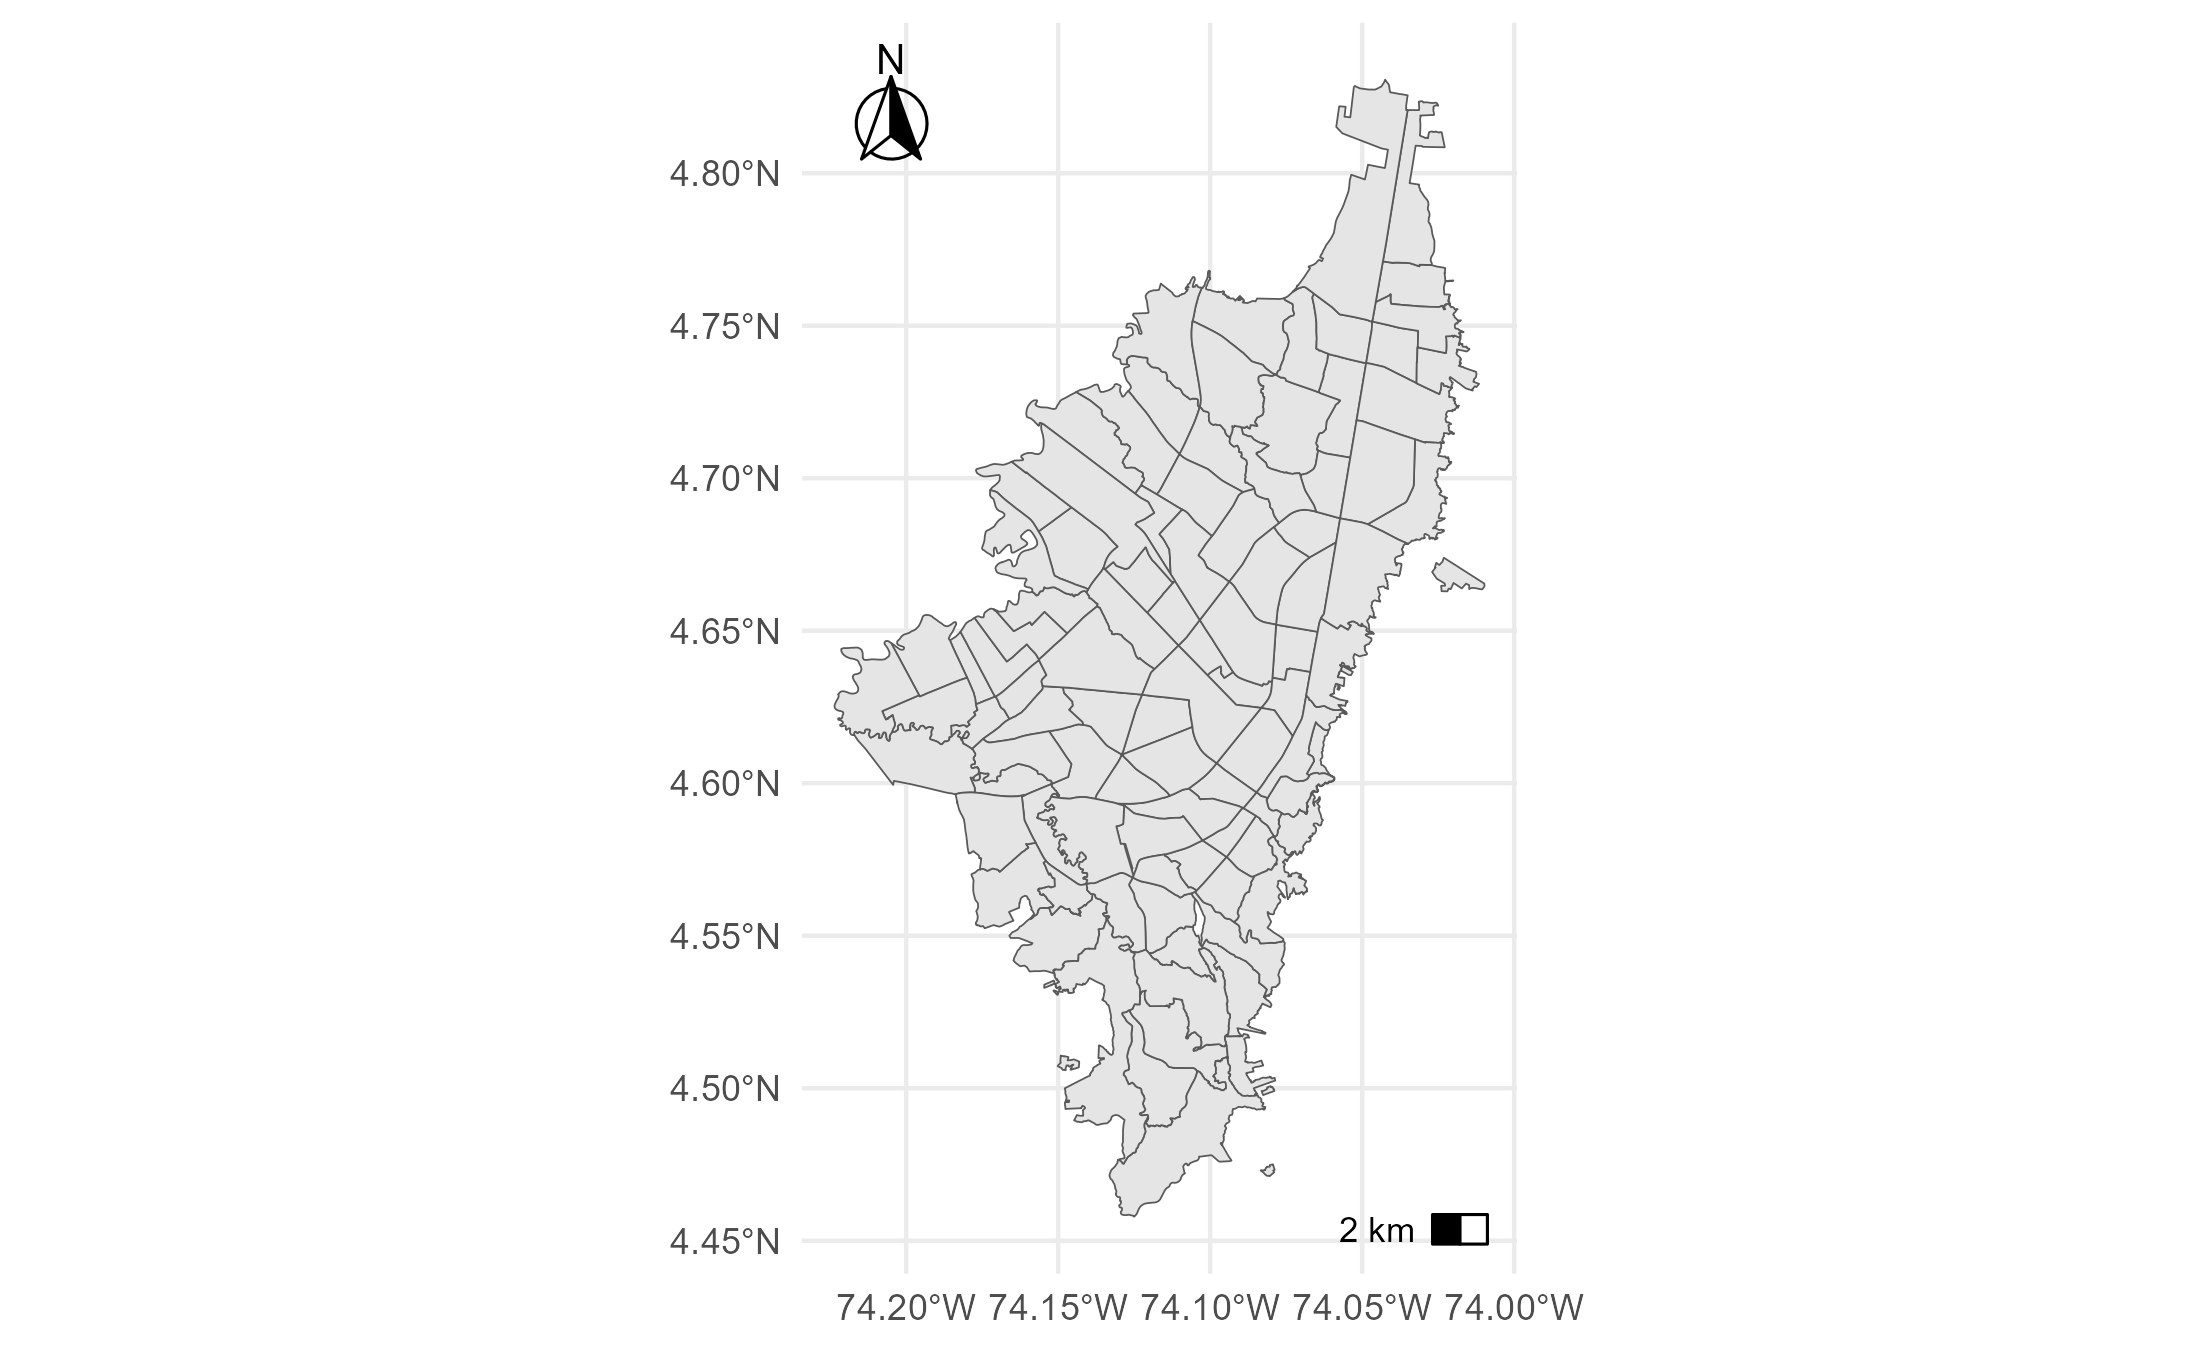
\includegraphics[width=16cm]{Data/Results/Images/Study_Area_UPZ.png}
    \caption{Bogotá boundary with ZPU local limits \citep{ secretariadistritaldeplaneacionCapaGeograficaEncuesta2023}}
    \label{fig:Study_Area_ZPU}
\end{figure}


\section{Spatial analysis unit}

The geographical analysis unit used in this study is a hexagon grid. The hexagon shape of the grid has convenient features when computing measures across different resolution spatial datasets. For example, having an equivalent distance from a hexagon of interest to their corresponding neighbouring hexagons generates more accurate time and distance operations between cells \citep{ubertechnologiesH3HexagonalHierarchical2023}. For example, Figure \ref{fig:Hex_grid_example} shows how a hexagon shape grid can aggregate spatial data, regardless of the features underlying geometries or boundaries of the spatial analysis units from the initial dataset. The spatial resolution of the grid used in this study has a level 9, representing an average area of 0.105 square kilometres \citep{ubertechnologiesH3HexagonalHierarchical2023}.

\begin{figure}[H]
    \centering
    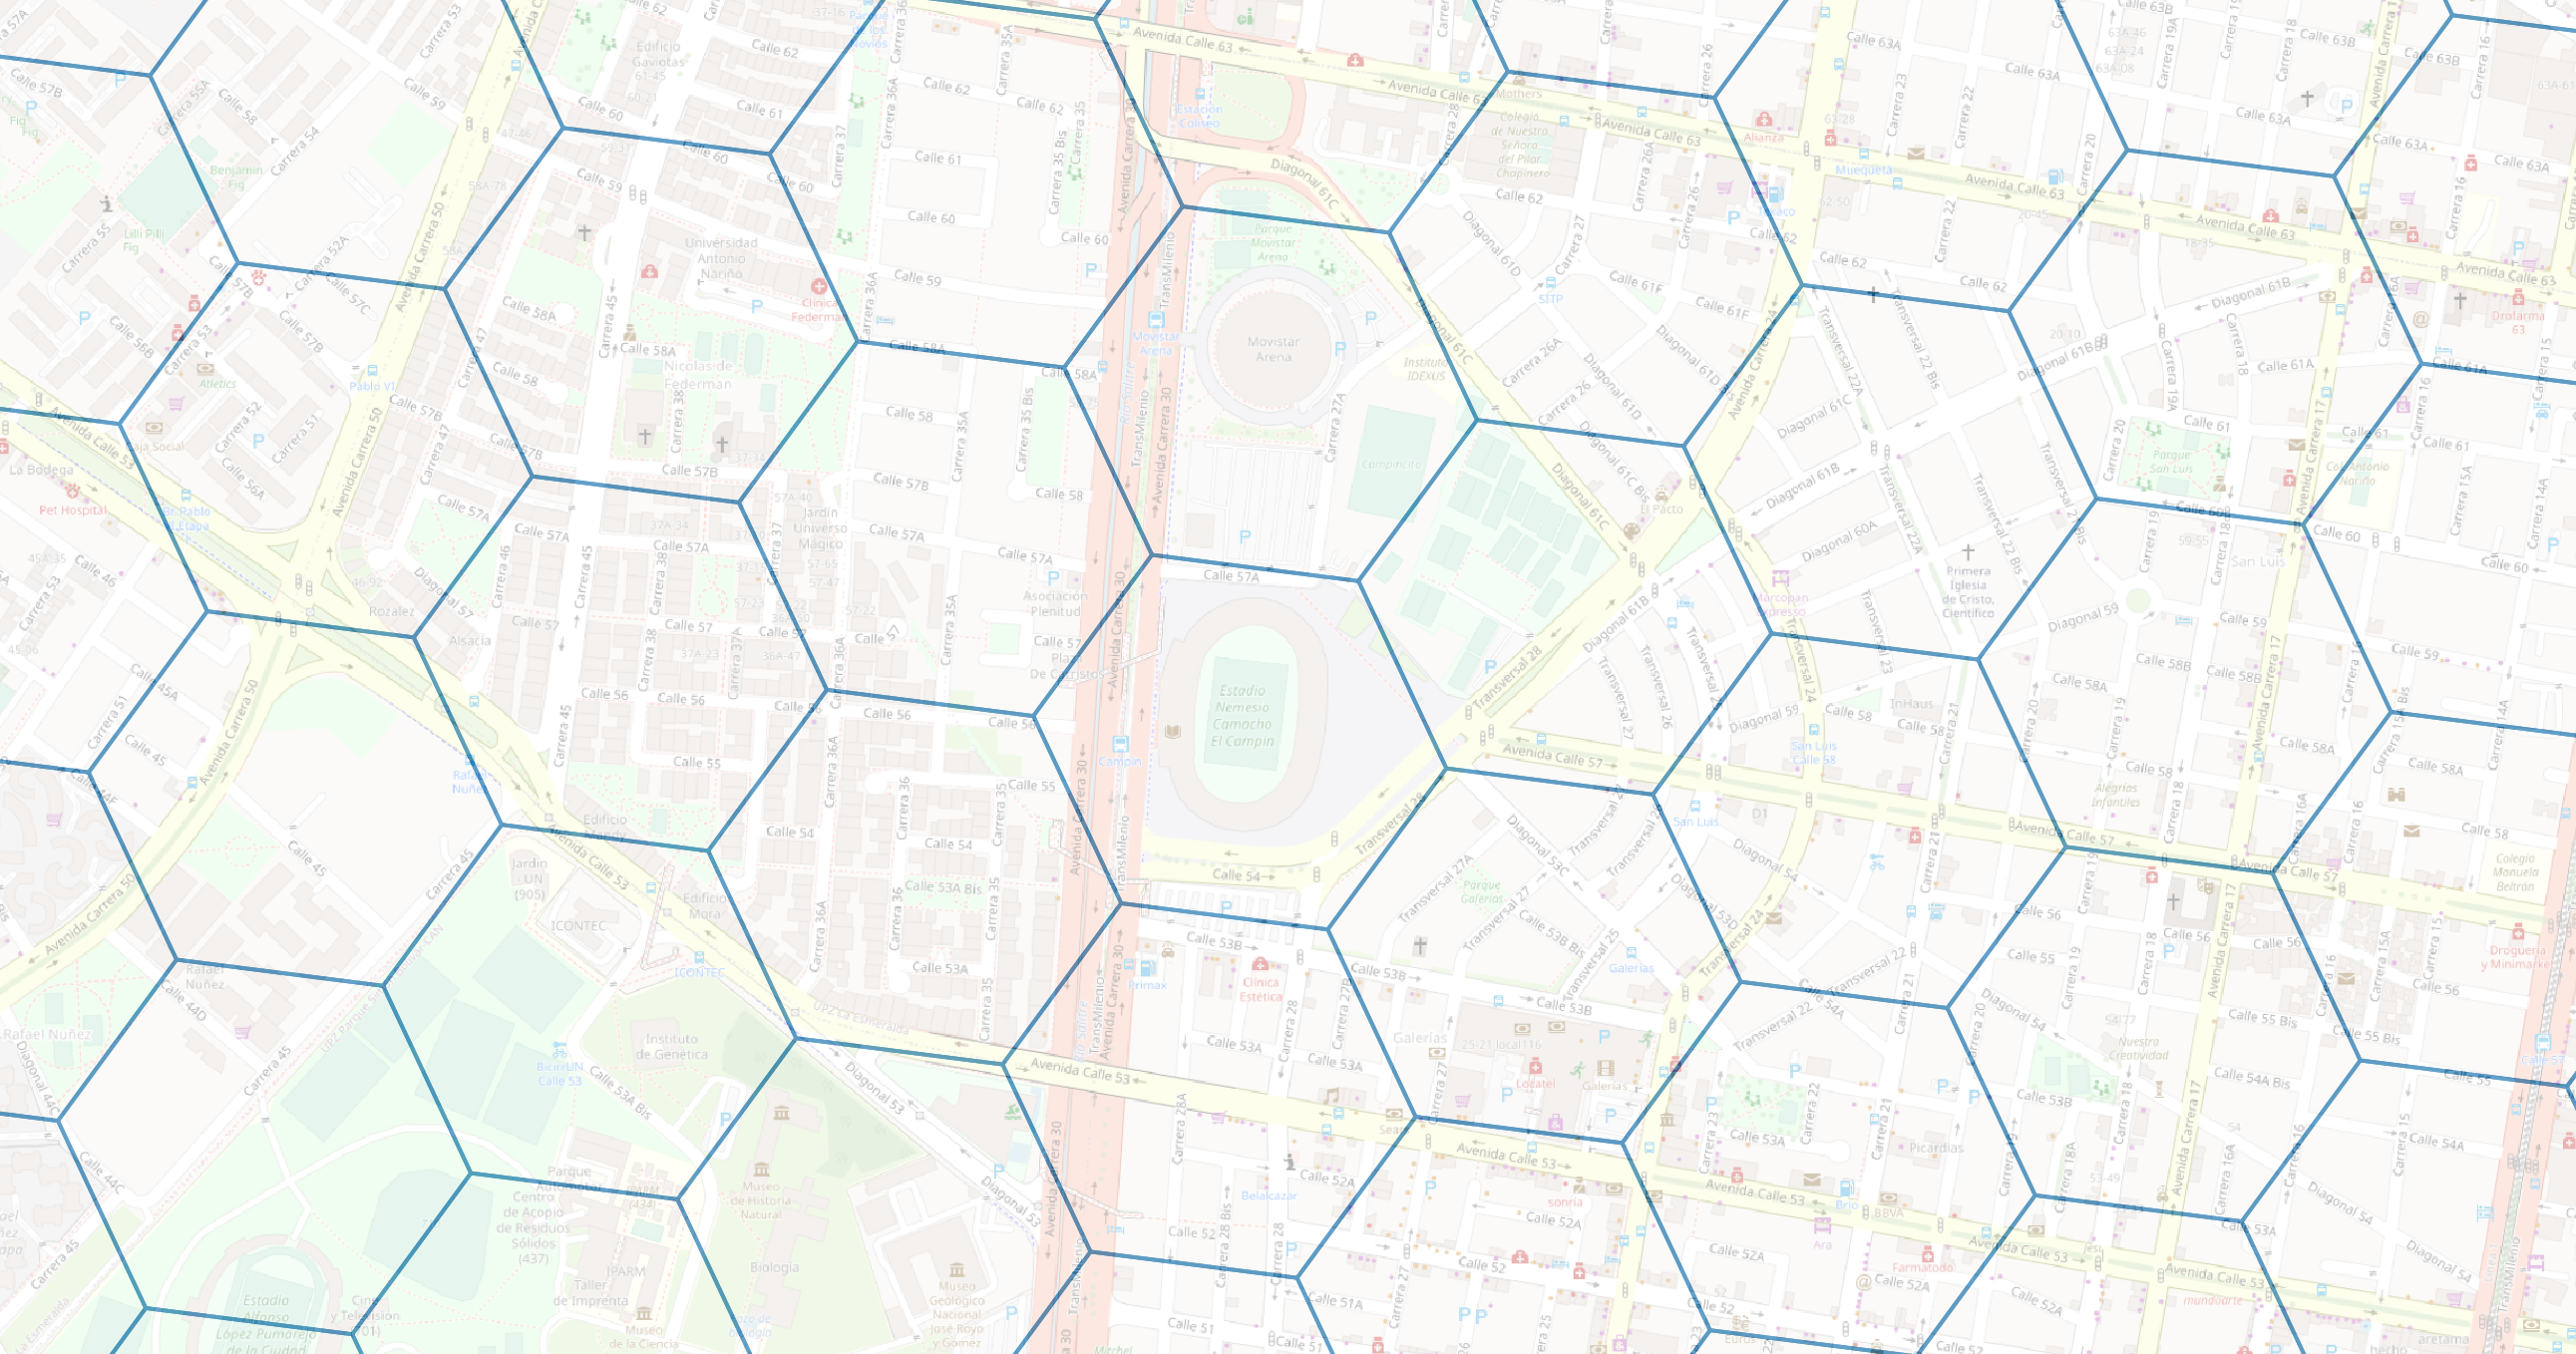
\includegraphics[width=10cm]{Images/Hex_grid.png}
    \caption{Resolution 9 hexagon grid example in Bogotá \citep{openstreetmapcontributorsPlanetDumpRetrieved2023a}}
    \label{fig:Hex_grid_example}
\end{figure}

\section{Workflow for data preparation}

To correctly model accessibility, transport infrastructure data, land use data and demographic data should be all combined in the same framework, as they are the main element influencing urban accessibility \citep{pereiraIntroductionUrbanAccessibility2023a}. Figure \ref{fig:Workflow_Summary} summarises the preprocessing workflow to transform the input data into the appropriate format data for the accessibility modelling. As described in Table \ref{tab:Data_summary}, the BRT data, the street network and the metro data will comprise the transport infrastructure component, while the land use data and the survey data will form the land use and demographic component, respectively.

\begin{figure}[H]
    \centering
    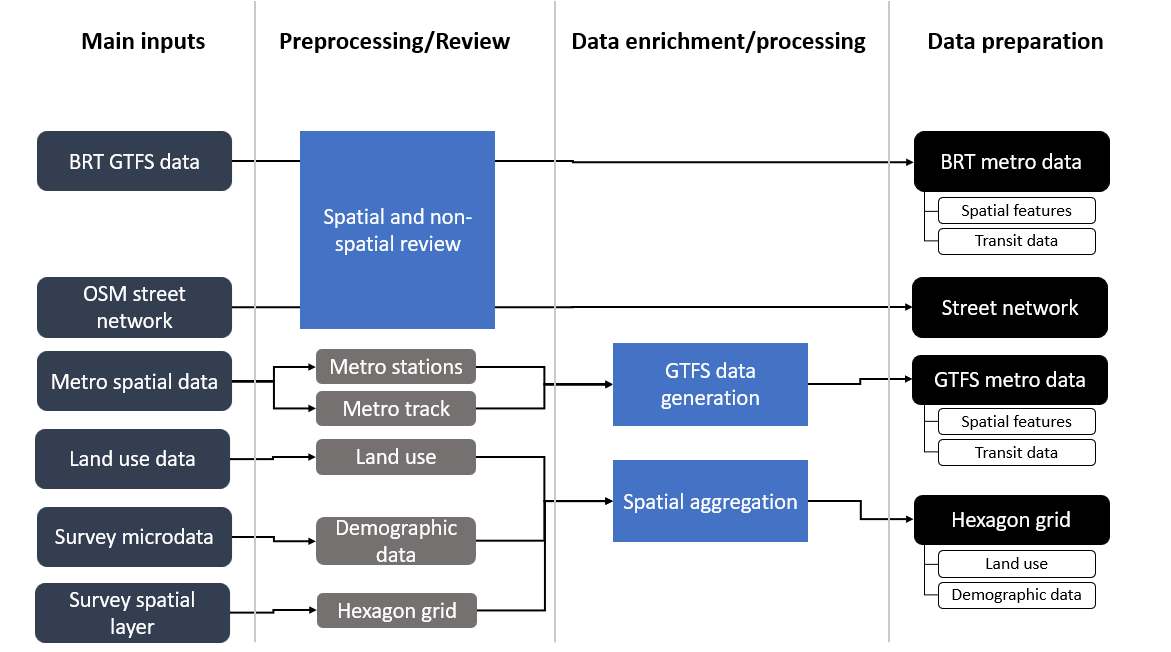
\includegraphics[width=13cm]{Images/Workflow_summary.png}
    \caption{Workflow summary diagram}
    \label{fig:Workflow_Summary}
\end{figure}

\section{GTFS data generation}

As this research aims to assess the accessibility impact of the future metro operation, the modelling process requires combining both modes of transportation in the same modelling exercise. Although the metro system is not yet operational, the metro transit data must be generated to be considered an available mode in the modelling process. Therefore, the metro transit information must be created with information about the infrastructure and the transit service published by the local authorities.

The current BRT transit information is already published in GTFS format by \citep{alcaldiadebogotad.c.EstacionesPrimeraLinea2022,alcaldiadebogotad.c.TrazadoPrimeraLinea2022} and previous reference of GTFS data for multimode transport modelling exercises \citep{pereiraIntroductionUrbanAccessibility2023a}, the metro transit data must be structured in GTFS format. The next subsections highlight the main spatial and alphanumeric procedures to generate the man tables of the GTFS data for future metro transit operations, as presented in Figure \ref{fig:GTFS_structure}.

The structuring and generation of the GTFS table were made considering the official GTFS specification \citep{mobiltydataGeneralTransitFeed2023} and the previous application made by \cite{pereiraIntroductionUrbanAccessibility2023a}.

\subsection{Agency}

The agency table in the GTFS data structure contains general information on the provider entity of the transit services. As Bogotá Metro company already exists, the agency table contains their already known information.


\begin{table}[ht]
\centering
\renewcommand{\arraystretch}{1.5}
\resizebox{\textwidth}{!}{%
\centering
\begin{tabular}{llllll}
  \hline
  agency\_id & agency\_name & agency\_url & agency\_timezone & agency\_lang & agency\_phone \\ 
  \hline
  1 & Metro de Bogota & https://www.metrodebogota.gov.co/ & America/Bogota & es & (+57)601-555-33-33 \\ 
  \hline
\end{tabular}}
\caption{Metro agency table.}
\label{tab:Metro_Agency}
\end{table}

\subsection{Routes}

The scope of the current metro construction project includes the metro infrastructure for the first line, and so does the scope of this research. The track of the metro line draws a line in a north-south line in the east zone of Bogotá to further go to the southwest of the city, as shown in Figure \ref{fig:Metro_Network} . For modelling purposes, this research will consider to possible routes:

\begin{itemize}
\item South route: The southern route will begin in the station located further southwest of the city and finish in the station located further north.
\item North route: The northern route will start in the further north located station and end at the station further southwest in Bogotá.
\end{itemize}

\begin{table}[ht]
\centering
\renewcommand{\arraystretch}{1.5}
\resizebox{\textwidth}{!}{%
\begin{tabular}{llllllll}  % <--- Changed column specification, removed "r"
  \hline
  route\_id & route\_short\_name & route\_long\_name & route\_desc & agency\_id & route\_color & route\_text\_color & route\_type \\ 
  \hline
  M1\_001 & S\_001 & South & Main & 1 & FFFFFF & 000000 & 1 \\ 
  M1\_002 & N\_001 & North & Main & 1 & FFFFFF & 000000 & 1 \\ 
  \hline
\end{tabular}}
\caption{Metro routes table.}
\label{tab:Metro_Routes}
\end{table}

As shown in Table \ref{tab:Metro_Routes}, the route must include the general identification data from each route, together with the provider entity and the mode of transport of the transit service, in the agency\_id and route\_type fields, respectively. The agency\_id field has a "1" value, consequently with the value given with the agency\_id field in \ref{tab:Metro_Agency} to the service provided. In like manner, the value "1" in the route\_type field indicates the mode of transport of the route metro or subway \citep{mobiltydataGeneralTransitFeed2023}. 

\subsection{Trips}

The trips represent the service unit of the transit service. A trip for each route will be considered in the modelling as shown in Table \ref{tab:Metro_Trips}. Apart from the identification data from each trip, the trip data also include a reference to the shape table in the shape\_id field, which will be explained later.




\begin{table}[ht]
\centering
\renewcommand{\arraystretch}{1.5}
%\resizebox{\textwidth}{!}
\caption{Metro trips table.}
\label{tab:Metro_Trips}
\end{table}

\subsection{Calendar and Calendar Dates}

The calendar and calendar date table allows the transit planning practitioners to schedule with days of the week when will the service of a trip operates and what particular date can be a service included or omitted from the operation. The scheduling structure of the metro service was based on the published schedule of the current BRT service. Both tables for the metro service are presented in Table \ref{tab:Metro_Calendar} and Table \ref{tab:Metro_Calendar_Dates}, respectively.

\begin{table}[ht]
\centering
\resizebox{\textwidth}{!}{%
\begin{tabular}{lrrrrrrrll}
  \hline
  service\_id & monday & tuesday & wednesday & thursday & friday & saturday & sunday & start\_date & end\_date \\ 
  \hline
  1 &   0 &   0 &   0 &   0 &   0 &   0 &   1 & 20000101 & 20990101 \\ 
  2 &   1 &   1 &   1 &   1 &   1 &   0 &   0 & 20000101 & 20990101 \\ 
  3 &   1 &   1 &   1 &   1 &   1 &   0 &   0 & 20000101 & 20990101 \\ 
  4 &   1 &   1 &   1 &   1 &   1 &   0 &   0 & 20000101 & 20990101 \\ 
  5 &   1 &   1 &   1 &   1 &   1 &   0 &   0 & 20000101 & 20990101 \\ 
  6 &   1 &   1 &   1 &   1 &   1 &   0 &   0 & 20000101 & 20990101 \\ 
  7 &   1 &   1 &   1 &   1 &   1 &   1 &   0 & 20000101 & 20990101 \\ 
   \hline
\end{tabular}}
\caption{Metro calendar table.}
\label{tab:Metro_Calendar}
\end{table}

Using the service\_id field, the calendar table allows to establish different types of service scheduling by weekday in a specific date range. Similarly, the calendar dates table can add or remove a service from a specific date, according to the value in the exception\_type field.

\begin{table}[ht]
\centering
%\resizebox{\textwidth}{!}
\caption{Metro calendar date table.}
\label{tab:Metro_Calendar_Dates}
\end{table}

\subsection{Shapes}

The shape table contains the geometry of the path of the trip. As the track path of the future metro has already been published in a spatial format, the shape table data will be structured based on the publicly available geometry of the metro track. As the modelling will be based on the assumption of one trip for each of the north and south routes, the geometry of the trips will only differ in the sequential order in which they travel the path.

Table \ref{tab:Metro_Shapes} shows a preview of the result of converting the spatial data of the track path into the shape table GTFS format. The shapes table contains the longitude and latitude coordinates of the path in the shape\_pt\_lon and shape\_pt\_lat fields, respectively. Equally important, the table indicates the sequential order in which the transit service will travel the path with an ascending integer values sequence in the shape\_pt\_sequence field.

\begin{table}[ht]
\centering
\begin{tabular}{lrllr}
  \hline
shape\_id & shape\_dist\_traveled & shape\_pt\_lon & shape\_pt\_lat & shape\_pt\_sequence \\ 
  \hline
M1\_001 & 0.00 & -74.06046 & 4.667379 &   1 \\ 
M1\_001 & 30.15 & -74.06051 & 4.667112 &   2 \\ 
M1\_001 & 30.57 & -74.06051 & 4.667109 &   3 \\ 
M1\_001 & 30.99 & -74.06051 & 4.667105 &   4 \\ 
M1\_001 & 31.42 & -74.06051 & 4.667101 &   5 \\ 
M1\_001 & 31.84 & -74.06051 & 4.667098 &   6 \\ 
   \hline
\end{tabular}
\caption{Metro shapes table.}
\label{tab:Metro_Shapes}
\end{table}

\subsection{Stops}

The stops table in the GTFS data structure stores the location and identification data from the stations where the transport user can begin or end using the metro transportation mode. Again, the stop data is generated based on the locations of stations contained in the spatial station's data public by the Bogotá Metro. After converting from a spatial data structure to a GTFS data structure, Table \ref{tab:Metro_Stops} shows the stops table from the metro GTFS data.

\begin{table}[ht]
\centering
\resizebox{\textwidth}{!}{%
\begin{tabular}{lllllll}
  \hline
stop\_id & stop\_code & stop\_name & stop\_lat & stop\_lon & location\_type & zone\_id \\ 
  \hline
M01 & 01 & Cra 96-01 & 4.640571 & -74.17746 & 0 & 0 \\ 
M02 & 02 & Portal de las Américas-02 & 4.630021 & -74.17186 & 0 & 0 \\ 
M03 & 03 & Carrera 80-03 & 4.622248 & -74.16671 & 0 & 0 \\ 
M04 & 04 & Calle 42 Sur-04 & 4.615737 & -74.16042 & 0 & 0 \\ 
M05 & 05 & Kennedy-05 & 4.617298 & -74.15159 & 0 & 0 \\ 
M06 & 06 & Av Boyaca-06 & 4.618484 & -74.14063 & 0 & 0 \\ 
   \hline
\end{tabular}}
\caption{Metro stops table.}
\label{tab:Metro_Stops}
\end{table}

\subsection{Stop times}

The stops times table indicates the arrival and departure times at every station a trip goes through. Although the local authorities or the metro company have not published specific timetables for future trips, the general scheduling and time between stations can be inferred from the available data.

The metro company, jointly with Bogotá's city council, have stated that the metro line will travel at an average speed of 43 km/h, allowing the Bogotá population to travel from the station on the south edge of the line to the last station on the opposite north edge in 27 minutes \citep{metrodebogotaPrimeraLineaMetro2022}. After calculating the distance between the stations' locations and the average travel speed of the metro, it is possible to establish the estimated arrival and departure time at every station for every trip. As the trips differ in the order they go through the stations, the data generation process is essentially the same but sequentially inverted. Table \ref{tab:Metro_Stop_Times} shows an overview of the stop times table of a trip from the north route, coupled with the stop\_sequence field that indicates the order of the stations.


\begin{table}[ht]
\centering
\resizebox{\textwidth}{!}{%
\begin{tabular}{llllrr} % Removed the "r" column specifier
  \hline
  trip\_id & arrival\_time & departure\_time & stop\_id & stop\_sequence & timepoint \\ 
  \hline
  M1\_002\_N\_3\_M1\_002 & 08:00:00 & 08:00:00 & M01 & 1 & 0 \\ 
  M1\_002\_N\_3\_M1\_002 & 08:01:52 & 08:01:52 & M02 & 2 & 0 \\ 
  M1\_002\_N\_3\_M1\_002 & 08:03:19 & 08:03:19 & M03 & 3 & 0 \\ 
  M1\_002\_N\_3\_M1\_002 & 08:04:44 & 08:04:44 & M04 & 4 & 0 \\ 
  M1\_002\_N\_3\_M1\_002 & 08:06:08 & 08:06:08 & M05 & 5 & 0 \\ 
  \hline
\end{tabular}}
\caption{Metro stop times table.}
\label{tab:Metro_Stop_Times}
\end{table}

Important to realize that the arrival and departure times listed in Table \ref{tab:Metro_Stop_Times} assume that the transit user would be aboard instantly. Although unrealistic, this was kept intentionally in this matter. After reviewing the BRT GTFS data \citep{transmilenios.a.GTFSEstaticos202306212023}, the arrival and departure time of all BRT transit presented the same behaviour. Hence, for modelling proposes, the resulting metro GTFS data will reflect this similarly to prevent artificially affecting the competitiveness between modes.

\subsection{Frequencies}

The frequencies table accounts for how often the trips depart from their respective first station during the day. The frequency of travel will vary depending on the current commuting temporal patterns in Bogotá. According to \cite{alcaldiadebogotad.c.EncuestaMovilidad20192019}, the schedule will assume a peak hour between 5:30 and 9:00 am and 4:00 and 7:00 pm. During the peak and non-peak hours, the frequencies of the trips will be one every 3 minutes and one every 15 minutes, respectively. The seconds' values in the headwat\_secs field express the hourly differentiated schedule for the time ranges established in the start\_time and end\_time fields.

\begin{table}[ht]
\centering
\begin{tabular}{llllrr} % Removed the "r" column specifier
  \hline
  trip\_id & start\_time & end\_time & headway\_secs & exact\_times \\ 
  \hline
  M1\_001\_S\_3\_M1\_001 & 00:00:00 & 05:29:59 & 900 & 0 \\ 
  M1\_001\_S\_3\_M1\_001 & 05:30:00 & 08:59:59 & 180 & 0 \\ 
  M1\_001\_S\_3\_M1\_001 & 09:00:00 & 15:59:59 & 900 & 0 \\ 
  M1\_001\_S\_3\_M1\_001 & 16:00:00 & 18:59:59 & 180 & 0 \\ 
  M1\_001\_S\_3\_M1\_001 & 19:00:00 & 23:59:59 & 900 & 0 \\ 
  \hline
\end{tabular}
\caption{Metro frequencies table.}
\label{tab:Metro_Frequencies}
\end{table}


\section{Spatial aggregation}

% Refence to the hexagon grid

The study uses a hexagon grid as a common spatial observation unit for both the inputs and results of the accessibility modelling process. With the spatial land use information, the location of opportunities can be geographically represented using the hexagon according to the activity related to a land use category of interest. Similarly, the demographic data available can describe socioeconomic and living conditions features of the inhabitant's location in a given hexagon grid.

\subsection{Land use}

% Reference to spatial join + count
% Include map

The land use data published by \cite{alcaldiadebogotad.c.DestinoEconomicoPredominante2022} is a spatial shapefile format containing the registered perimeter boundary of all terrains. Each feature represented the geometry of the terrain, and the land use category was stored in a character column in the spatial dataset.

To aggregate land use data to the hexagon grid, the intersecting geometries of every terrain were counted and grouped by their respective land use case to count for the number of each land use terrain location within each hexagon grid. Henceforth, the resulting grid contained the terrain for every land use category. As the hexagon grid has a homogeneous area, the results can be interpreted as the terrain density by hexagon for the land use category of interest. Figure \ref{fig:Opportunities_Spatial} presents the resulting hexagon grid for the commercial corridor land use density.

\begin{figure}[H]
    \centering
    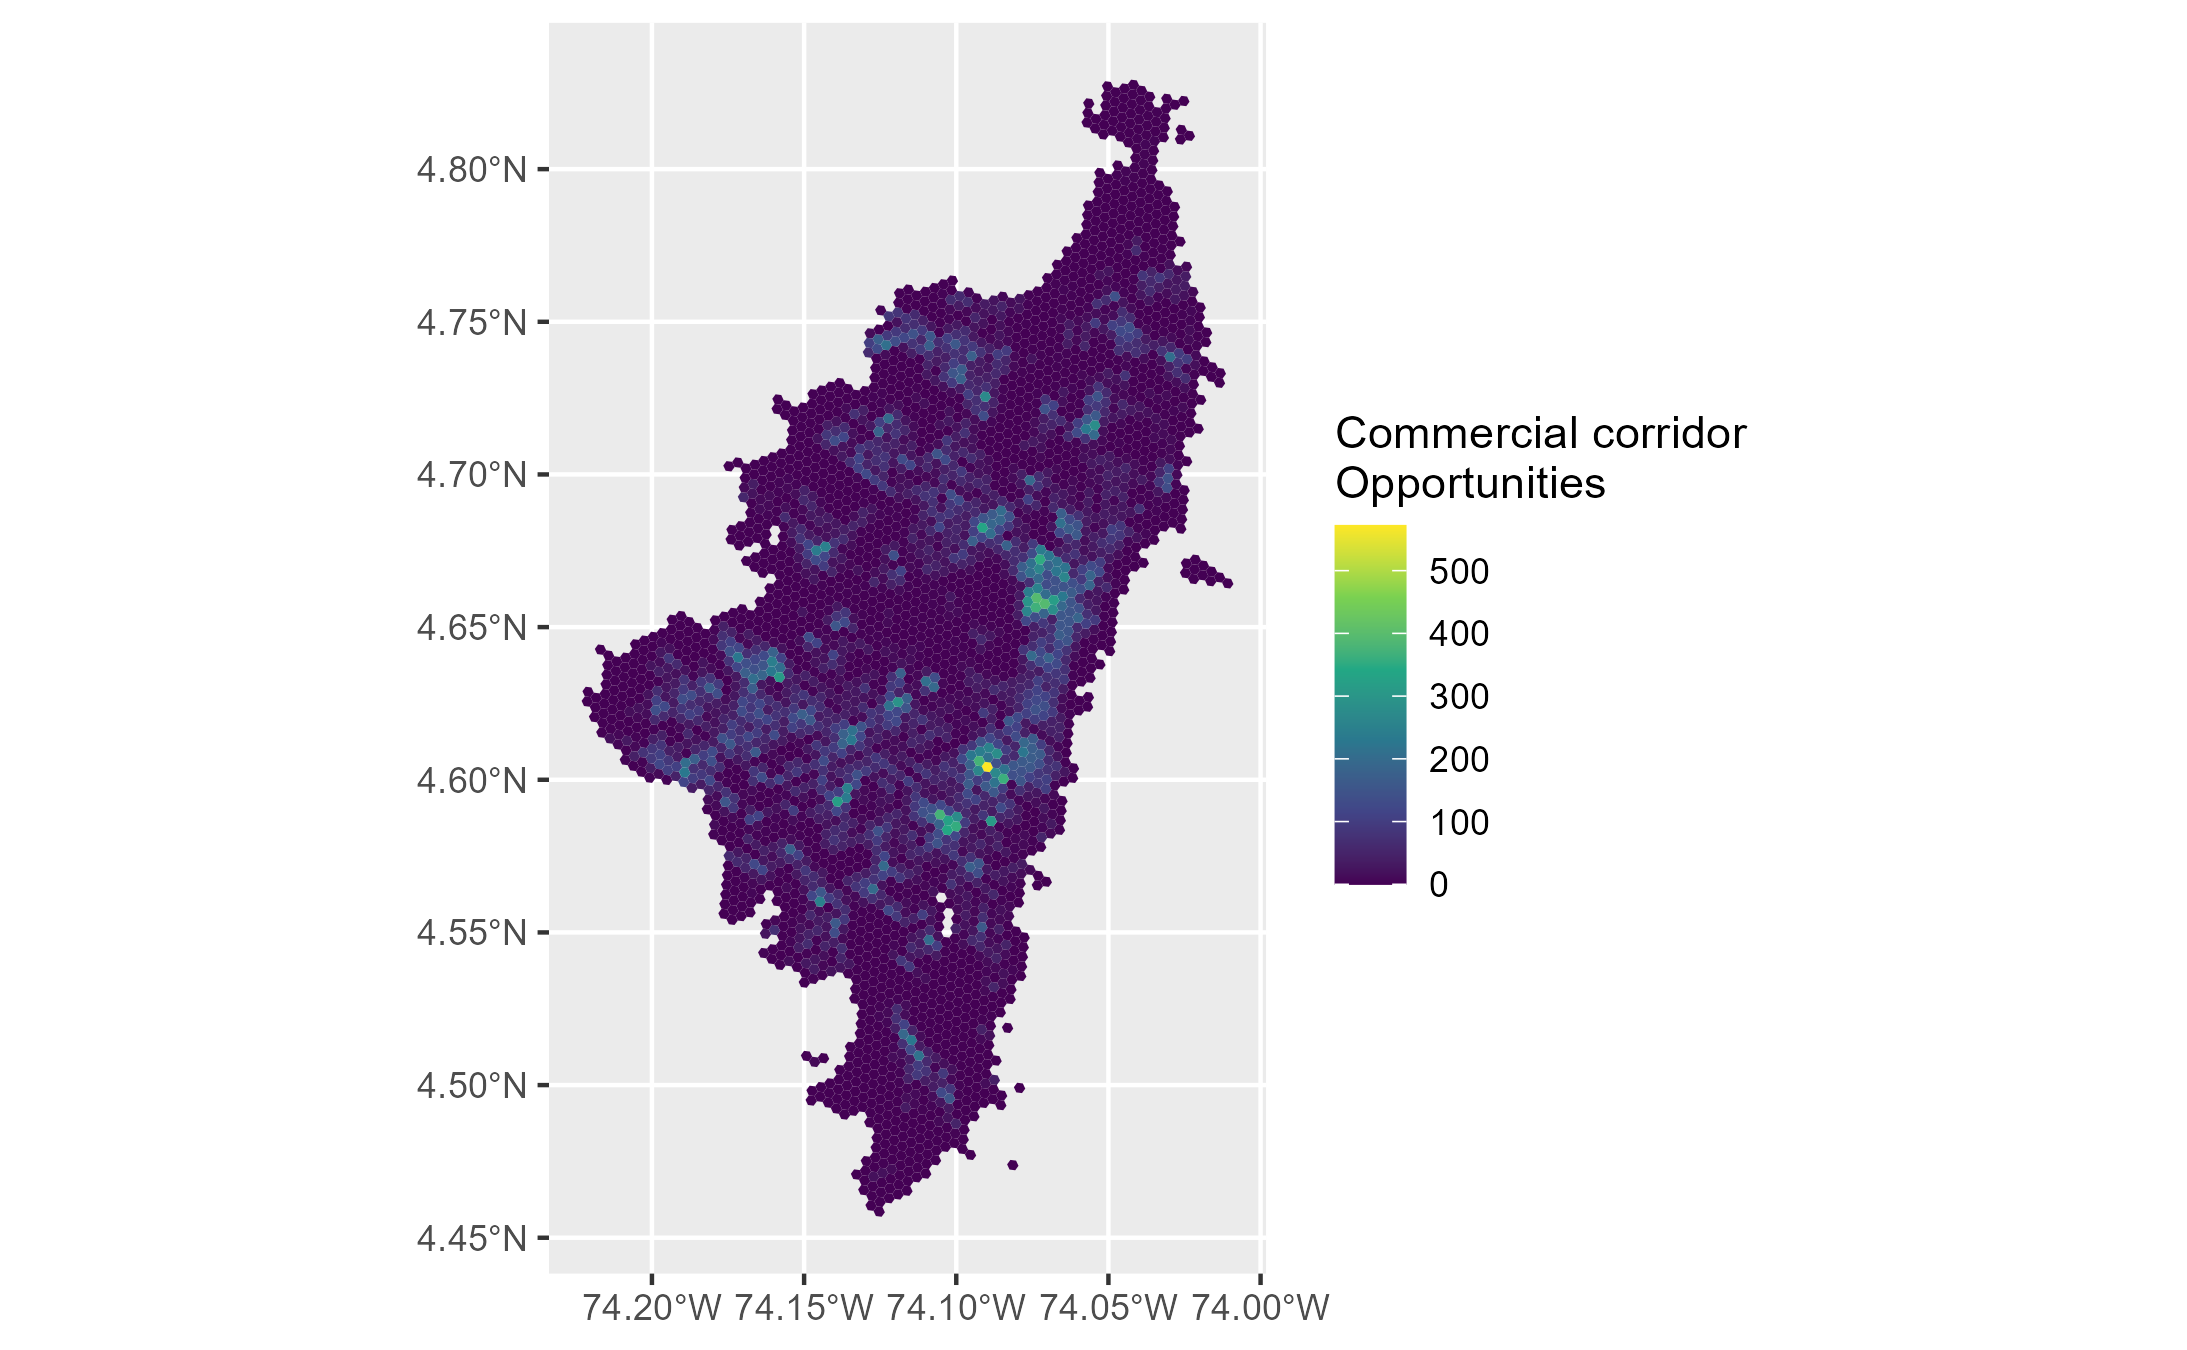
\includegraphics[width=13cm]{Data/Results/Images/Opportunities_COD_21.png}
    \caption{Spatial commercial corridor land use density}
    \label{fig:Opportunities_Spatial}
\end{figure}

% Refefence of where are the opportunities in bogota

\subsection{Demographics}

The aggregation of demographic data to the hexagon would allow the assessment of socioeconomic variables of Bogotá's inhabitants across space. This study will incorporate income data gathered by \cite{secretariadistritaldeplaneacionMicrodatosEncuestaMultiproposito2023} to the hexagon grid.

The income data used in this study was initially in a non-spatial format. First, it was grouped and georeferenced using the ZPU that \cite{secretariadistritaldeplaneacionMicrodatosEncuestaMultiproposito2023} provided. Second, the household average income was calculated considering the a household could have multiple members that generate income. Third, the overall ZPU income average vas calculated and integrated with the corresponding ZPU spatial layer. Finally, the mean hexagon income was computed using an area-weighted average. As the boundaries of the ZPU are disparate and uneven, the income value computed for the hexagon results from a weighted average using the income value of each ZPU and the percentage or intersection area of each ZPU, respectively. 

Figure \ref{fig:Income_Decile_Hex} shows the resulting hexagon grid after the spatial aggregation and after grouping the hexagons by income deciles.

\begin{figure}[H]
    \centering
    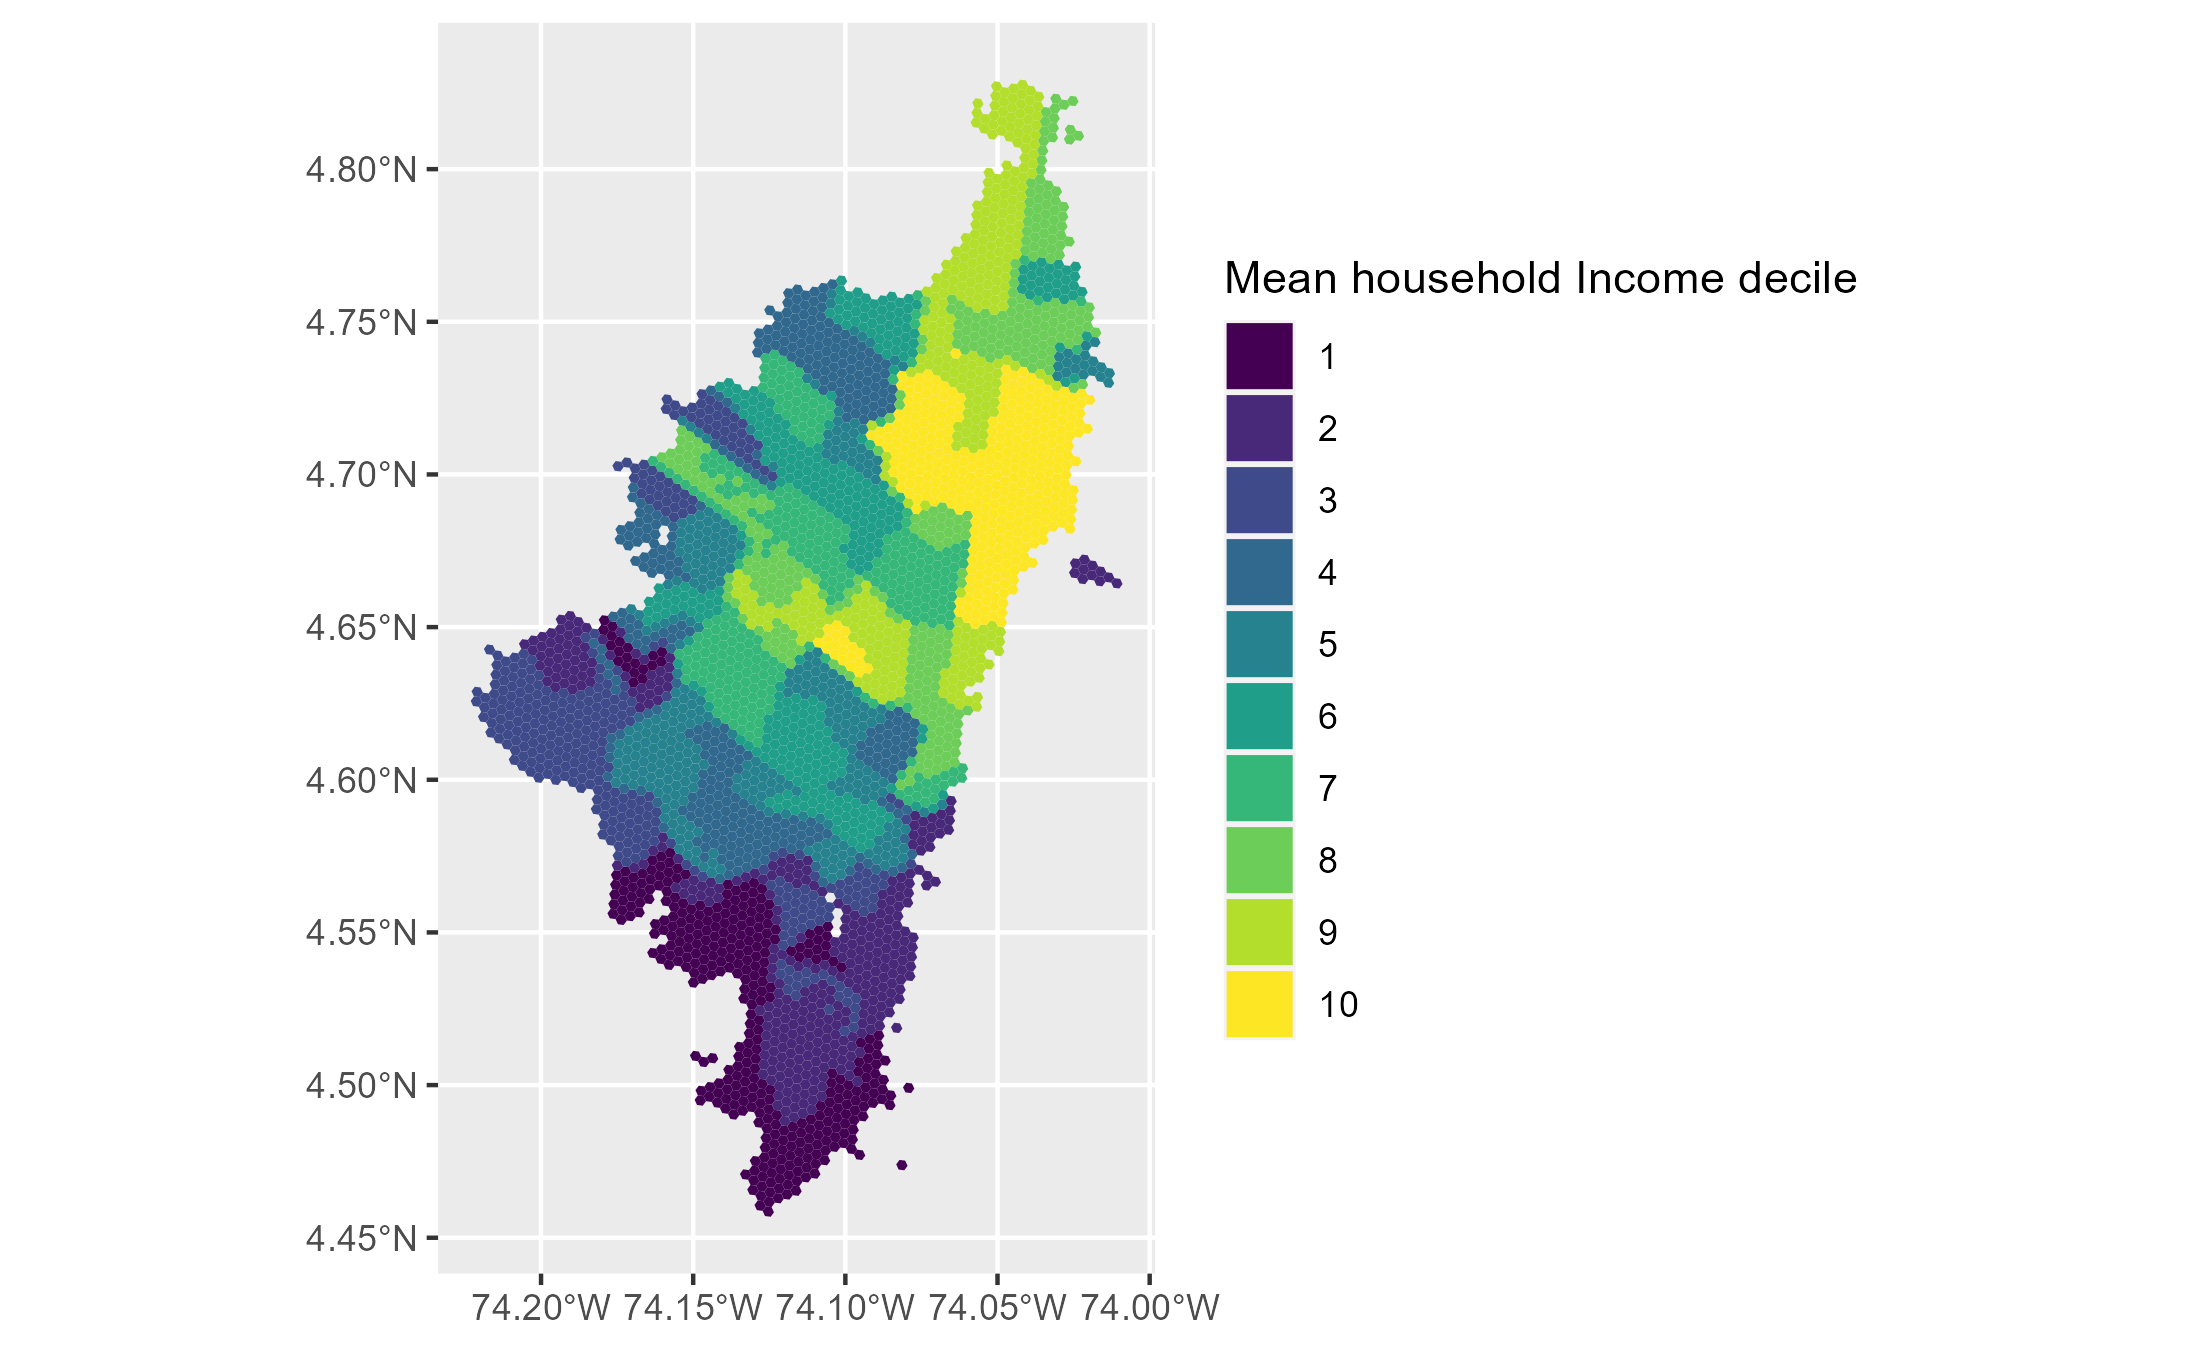
\includegraphics[width=13cm]{Data/Results/Images/Demo_income_decile_discrete.png}
    \caption{Resulting hexagon grid average household income decile}
    \label{fig:Income_Decile_Hex}
\end{figure}


\section{Accessibility measure}

The accessibility measure chosen to model is a cumulative active accessibility measure. The cumulative accessibility measure accounts for the number of opportunities a person can reach from a given origin location without surpassing the predefined threshold. In other, word cumulative accessibility measures how many opportunities a person can access given their location, the opportunities for spatial distribution and the transit operation.

According to \cite{pereiraIntroductionUrbanAccessibility2023a}, the cumulative accessibility measure can be fine as follows:

\[A_{i}=\sum_{j=1}^{n} O_{j} \times f(c_{ij})\]

\[f(c_{ij})=\begin{cases}
1, & \text{if $c_{ij}$ < $C$}.\\
0, & \text{Otherwise}.
  \end{cases}
\]

where

\begin{itemize}
    \item $A_{i}$ in the accessibility at origin location $i$.
    \item $O_{j}$ is the number of opportunities located at destination $j$.
    \item $n$ is the total number of destinations.
    \item $f(c_{ij})$ is a function that takes 0 or 1 values if the travel cost $c_{ij}$ value from origin $i$ to destination $j$ has exceeded the $C$ travel cost limit. 
\end{itemize}


\section{Scenarios} \label{Scenarios}

This study examined the current and future accessibility scenarios as presented in Figure \ref{fig:Method_Summary}. On the one hand, the current scenario consists of the current transit operation and infrastructure composed of the BRT and street networks. On the other hand, the future scenario will include the BRT and street network, together with the future transit operation and infrastructure for the metro.

Important to notice that the street network was used to have street infrastructure through which the modelling could compute travel by walking. It does not consider any other type of motorized transportation use apart from the BRT network. Additionally, single-mode scenarios were also considered in the accessibility modelling. For control purposes, accessibility for BRT, metro and walking modes was calculated individually to assess accessibility in a disaggregated manner.

\section{Accessibility modelling}

The cumulative accessibility modelling was calculated using the R5R library with R Programing Language. The library calculates accessibility by performing tree procedures. Next, each procedure is described indicating the inputs required for each one:

\begin{enumerate}
    \item Building multi-mode network: Based on the GTFS data and the street network, a multi-transport mode is built to connect origins and destinations according to the infrastructure available.
    \item Time travel matrix computation: The travel time between all origin and destination combinations is computed, favouring the fastest mode combination available.
    \item Apply cost travel thresholds: According to the threshold parameters, the destination locations are filtered so the accessibility results account for only the destination within the travel cost limits.
\end{enumerate}


\subsection{Inputs} \label{Inputs}

The input data provided for each scenario should be aligned with the transit and infrastructure each scenario aim to model. Table \ref{tab:Inputs_By_Scenario} indicates with a check mark the inputs considered for the before and after scenarios as described in \ref{fig:Method_Summary}, together with the additional control scenarios stated in subsection \ref{Scenarios}.


\begin{table}[H]
\centering
\begin{tabular}{c|ccc}
\hline
\multicolumn{1}{l|}{} & \multicolumn{3}{c}{\textbf{Inputs}}                                                   \\ \hline
\textbf{Scenario}     & \multicolumn{1}{l}{\textbf{Street network}} & \textbf{BRT GTFS} & \textbf{Metro GTFS} \\ \hline
Current         & \checkmark & \checkmark &       \\ \hline
Future          & \checkmark & \checkmark & \checkmark \\ \hline
Walking only    & \checkmark &       &       \\ \hline
Metro + walking & \checkmark &       & \checkmark \\ \hline
\end{tabular}
\caption{Input data by scenario.}
\label{tab:Inputs_By_Scenario}
\end{table}

\subsection{Parameters}

% Reference to the threshold

The parameters of the accessibility modelling procedure allow configuring the transit and commuting conditions considered in the urban accessibility computation. Among the conditions that the R5R parameters can simulate in the accessibility modelling are the maximum walking duration and the total maximum commuting duration. Considering the average travel times when using one motorized transit mode in Bogotá \citep{alcaldiadebogotad.c.EncuestaMovilidad20192019}, the maximum walking time and total trip duration had values of 30 and 60 minutes, respectively.

\chapter{Results} \label{Chap5}

\section{Accessibility by scenario}

The accessibility results show the number of reachable opportunities within a travel cost threshold from every possible origin location. The measure was calculated by every scenario described in sections \ref{Scenarios} and \ref{Inputs}, where the scenarios and inputs for the modelling were defined, respectively.

% Hide working figure
% \begin{figure}[H]
%     \centering
%     \begin{minipage}{0.45\textwidth}
%         \centering
%         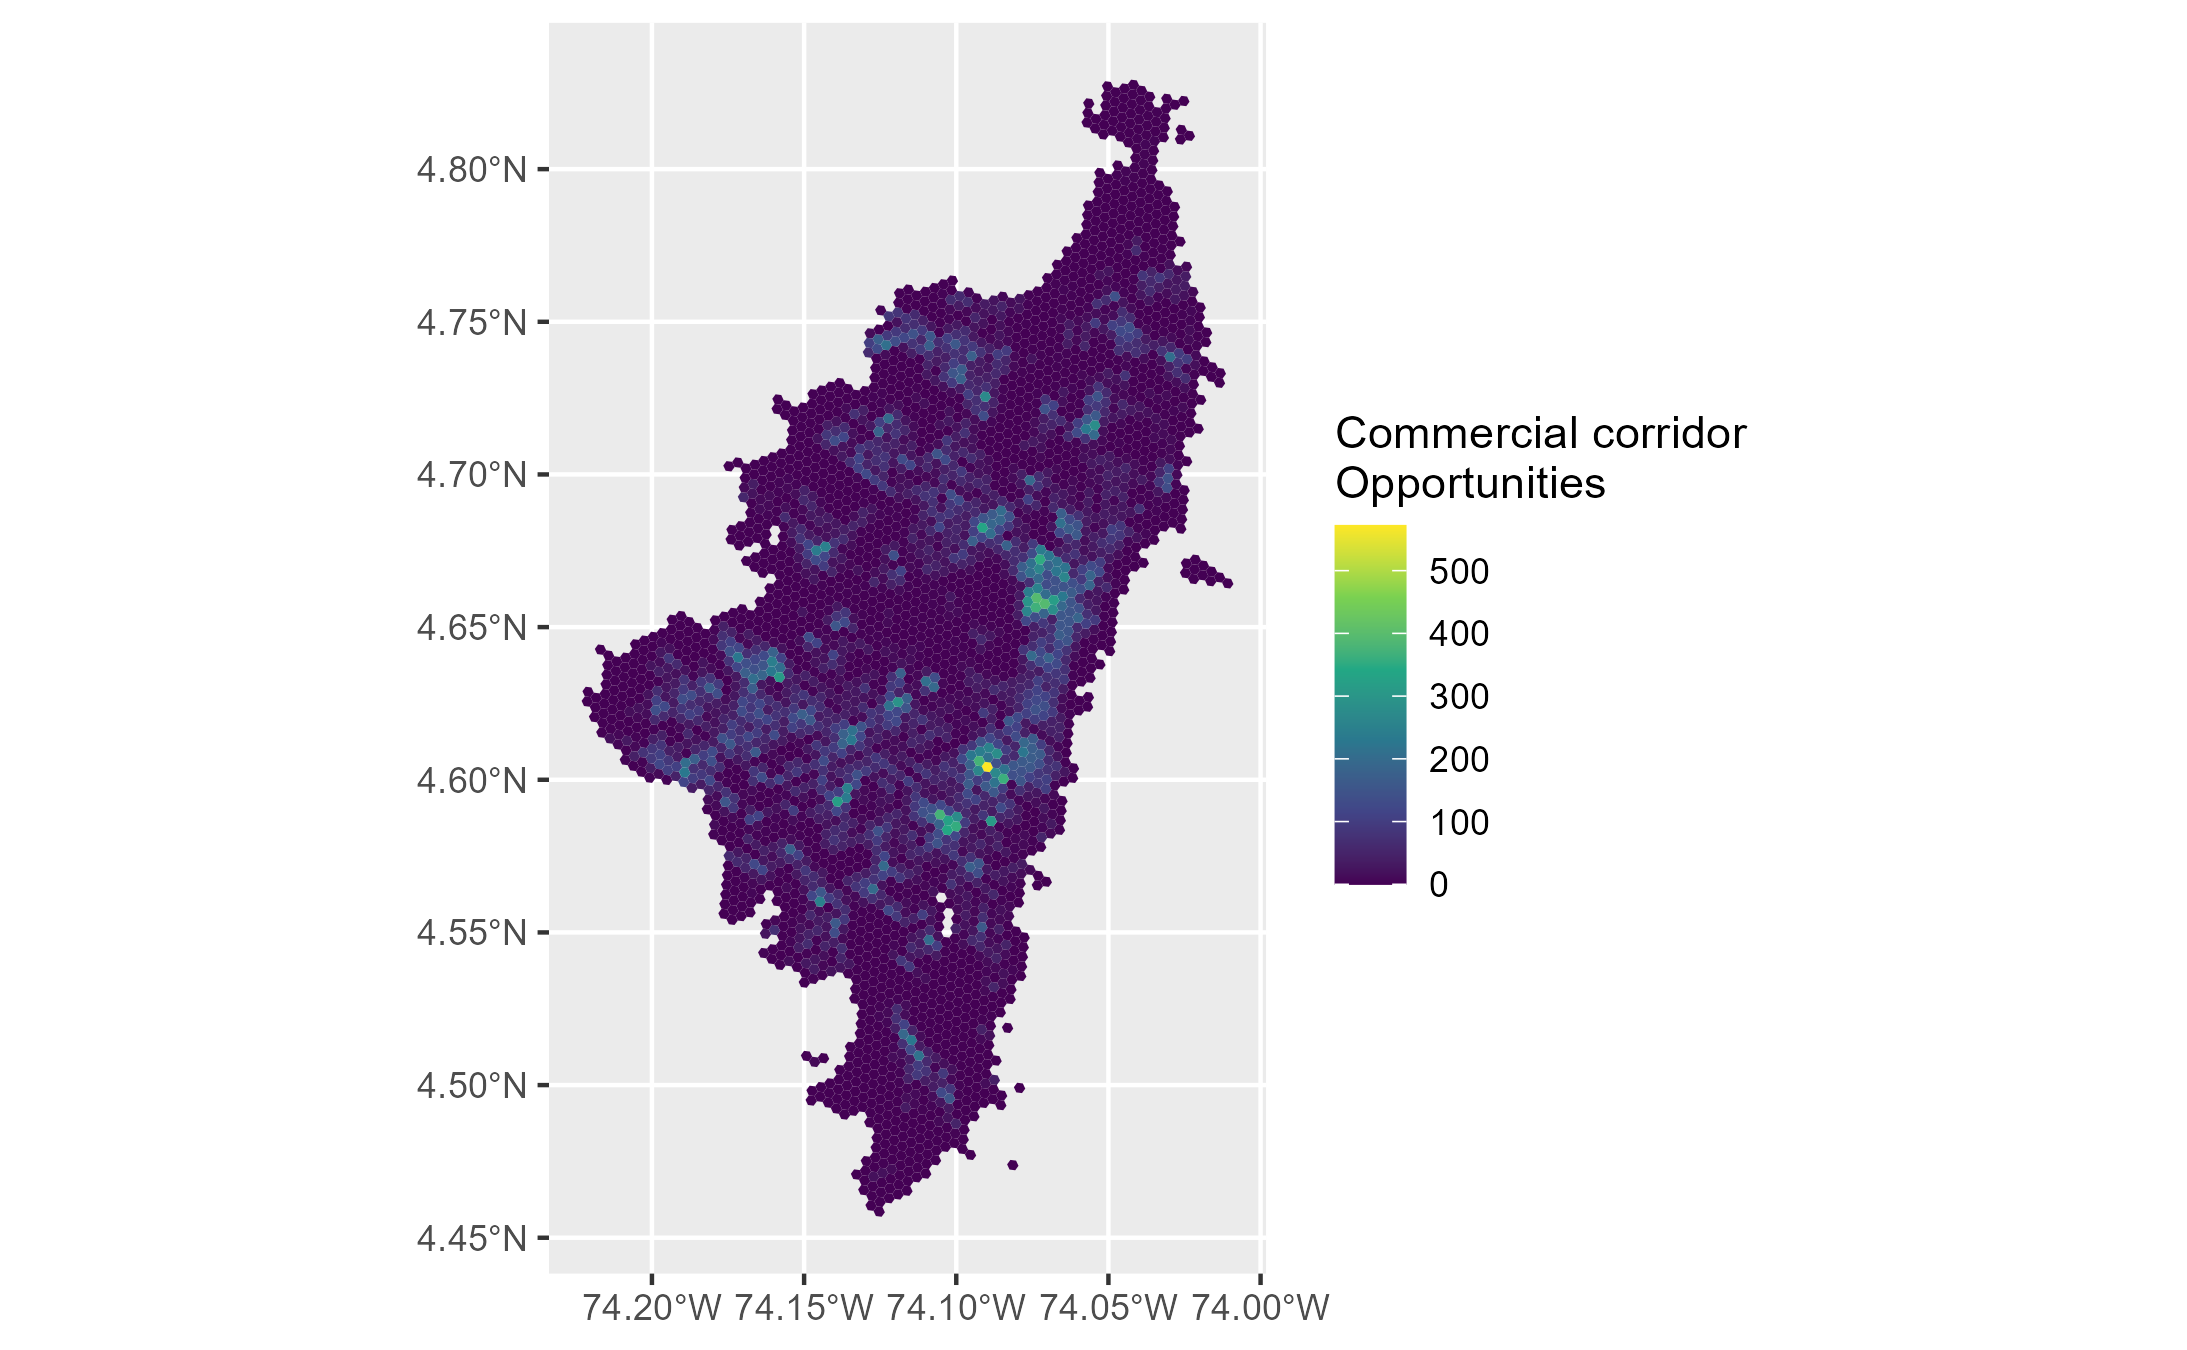
\includegraphics[width=1.3\linewidth]{Data/Results/Images/Opportunities_COD_21.png}
%          \caption{Opportunities}
%         \label{fig:Results_Opportunities}
%     \end{minipage}%
%     \hfill
%     \begin{minipage}{0.45\textwidth}
%         \centering
%         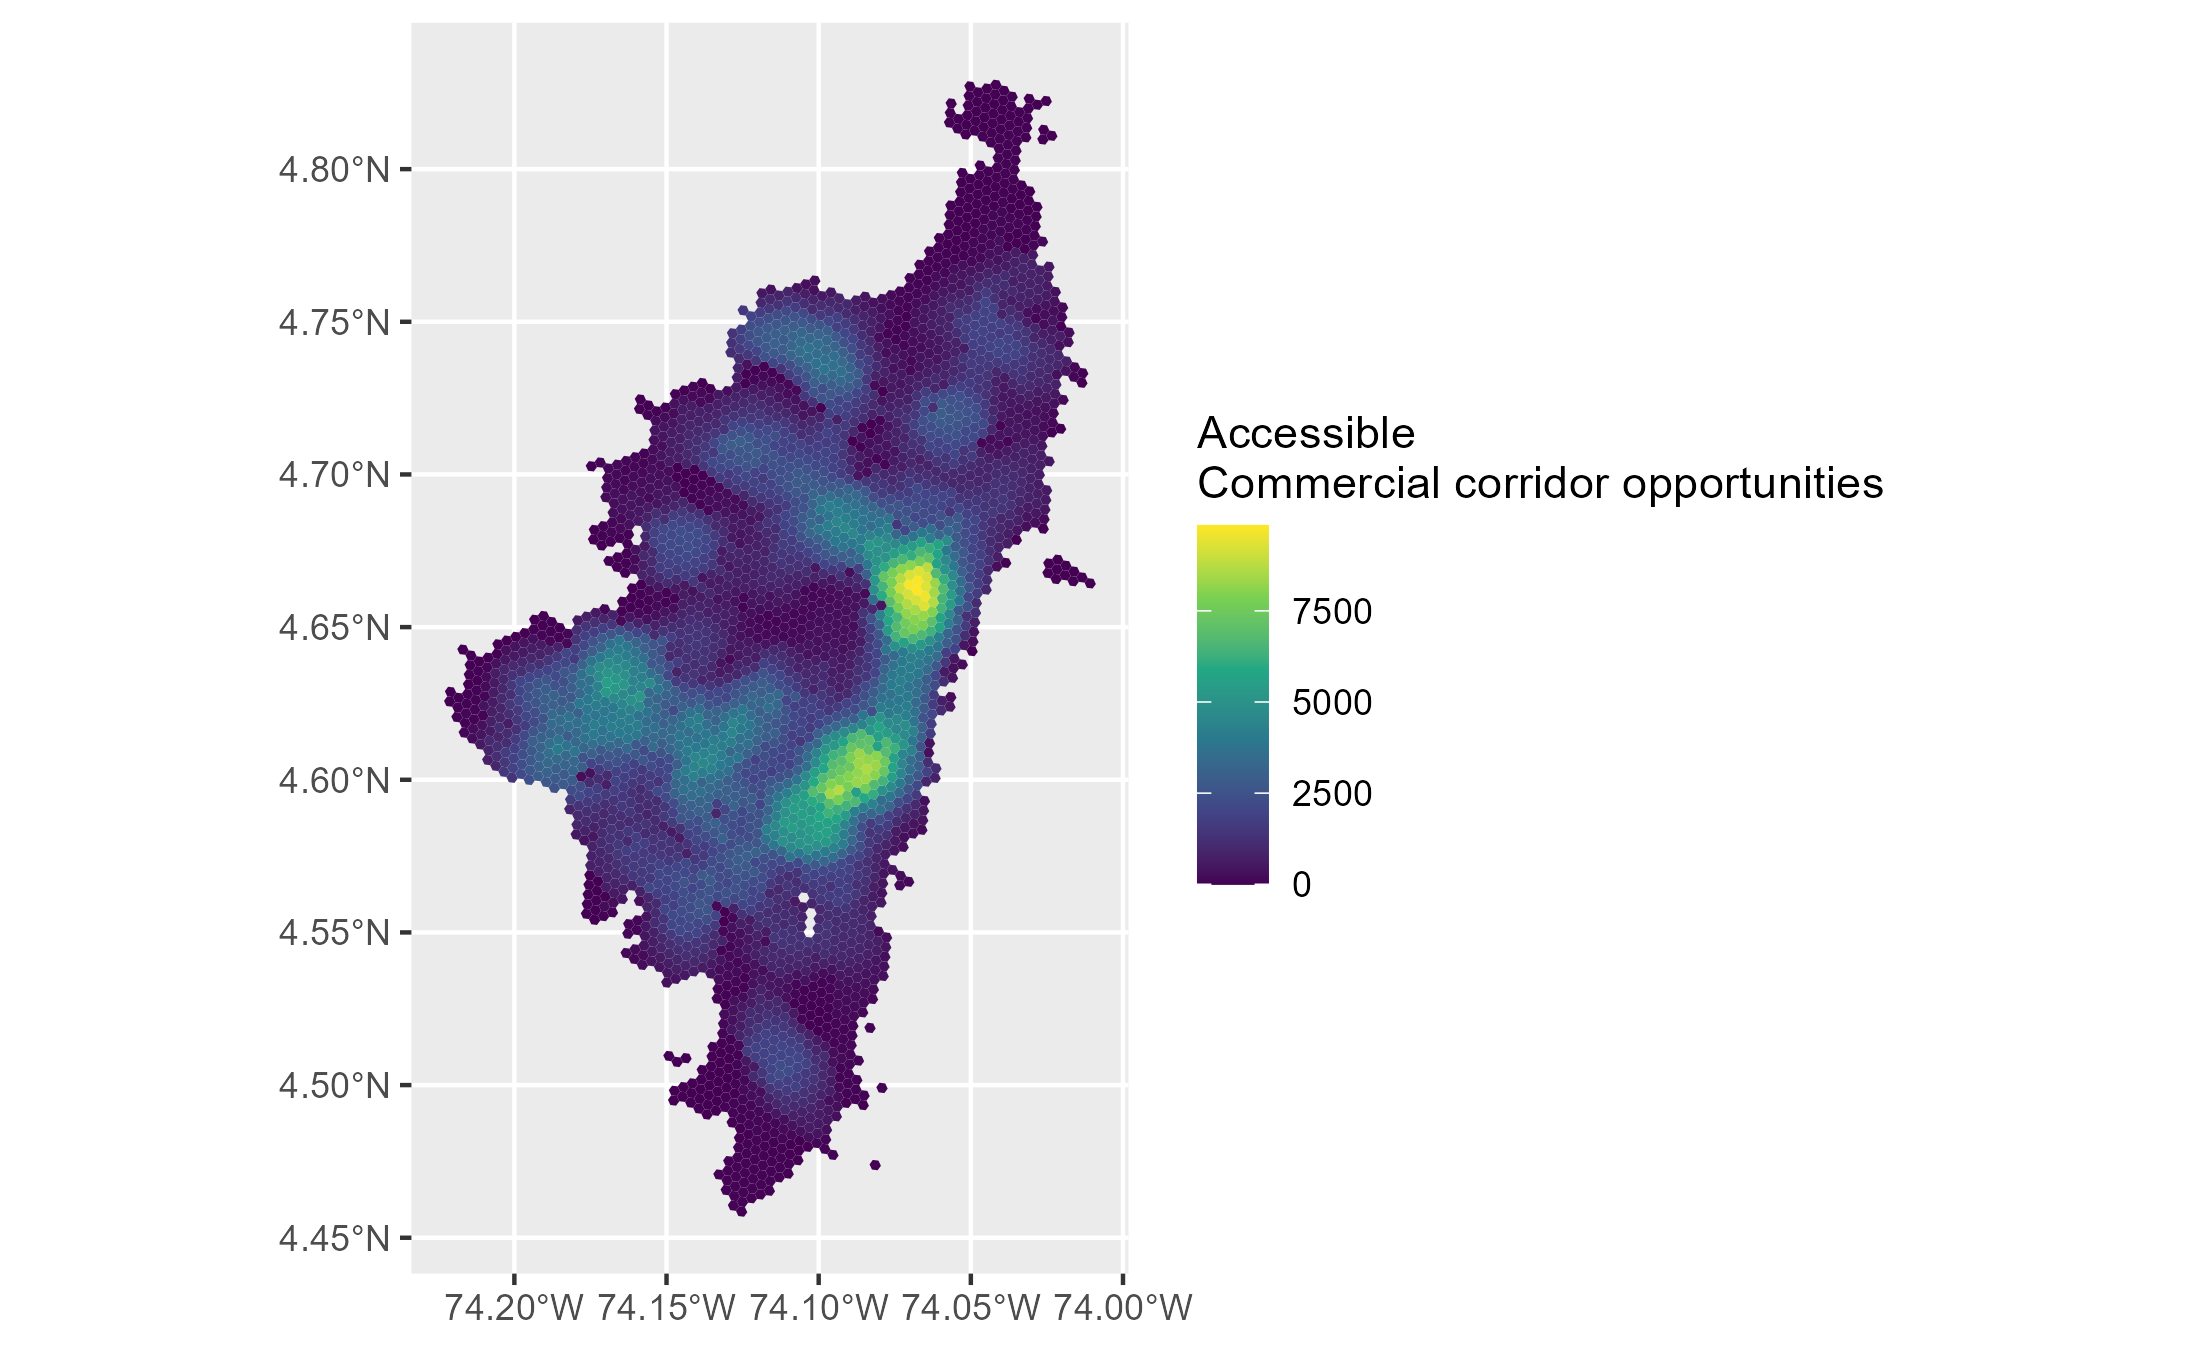
\includegraphics[width=1.3\linewidth]{Data/Results/Images/Access_Walk_base.png}
%         \caption{Walking}
%         \label{fig:Results_Walking}
%     \end{minipage}
%     \centering
%     \begin{minipage}{0.45\textwidth}
%         \centering
%         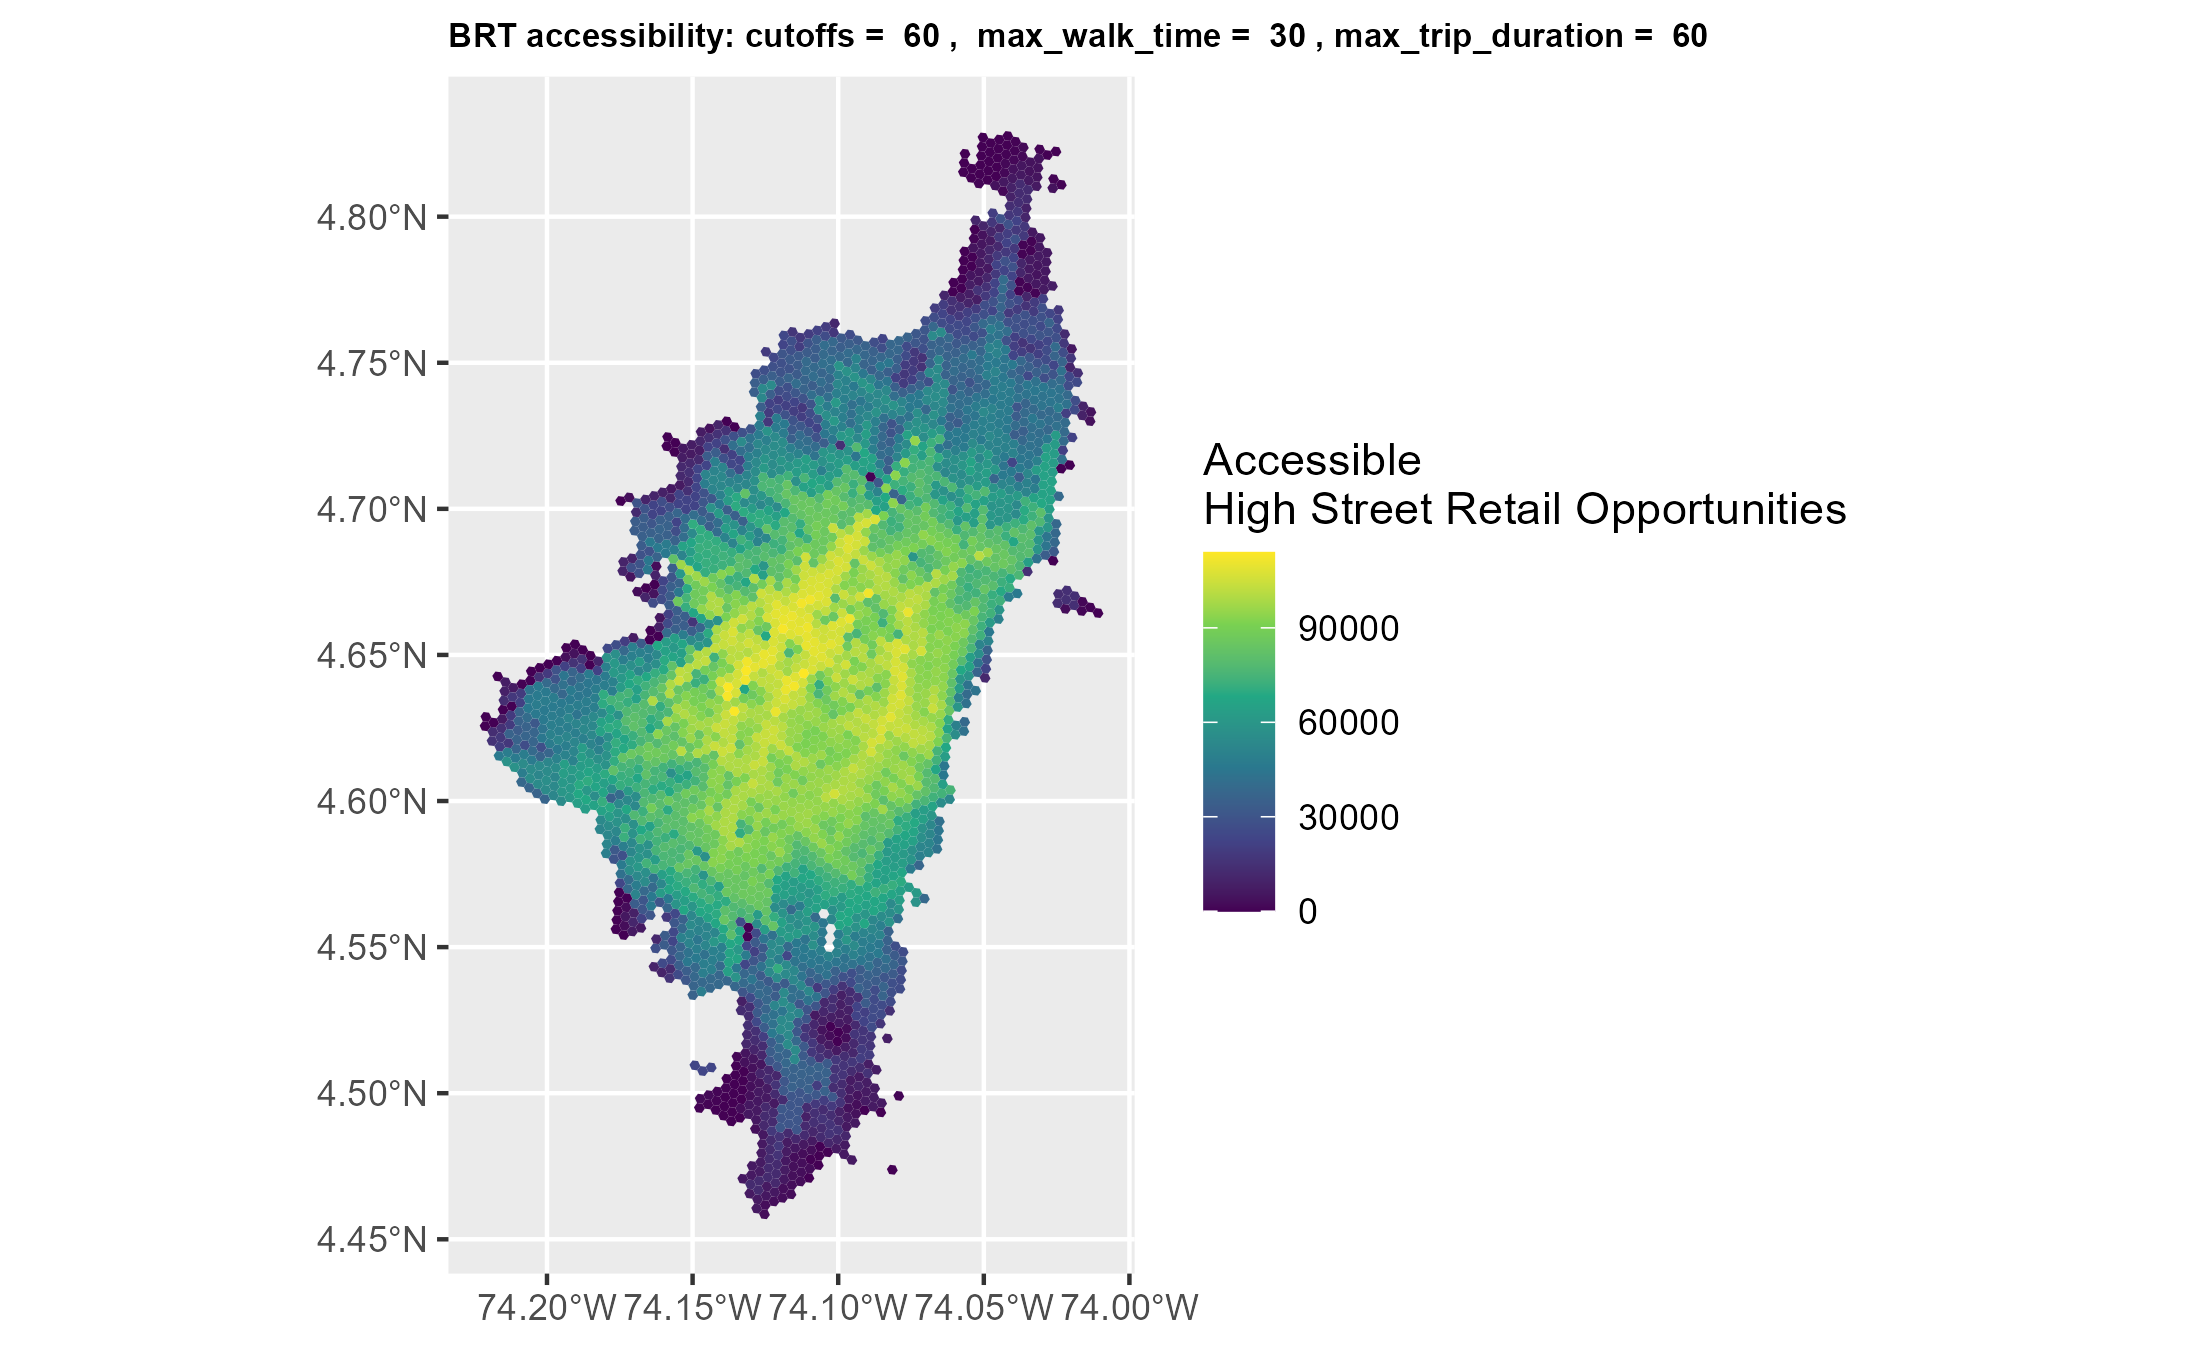
\includegraphics[width=1.3\linewidth]{Data/Results/Images/Access_BRT_base.png}
%          \caption{BRT}
%         \label{fig:Results_Opportunities}
%     \end{minipage}%
%     \hfill
%     \begin{minipage}{0.45\textwidth}
%         \centering
%         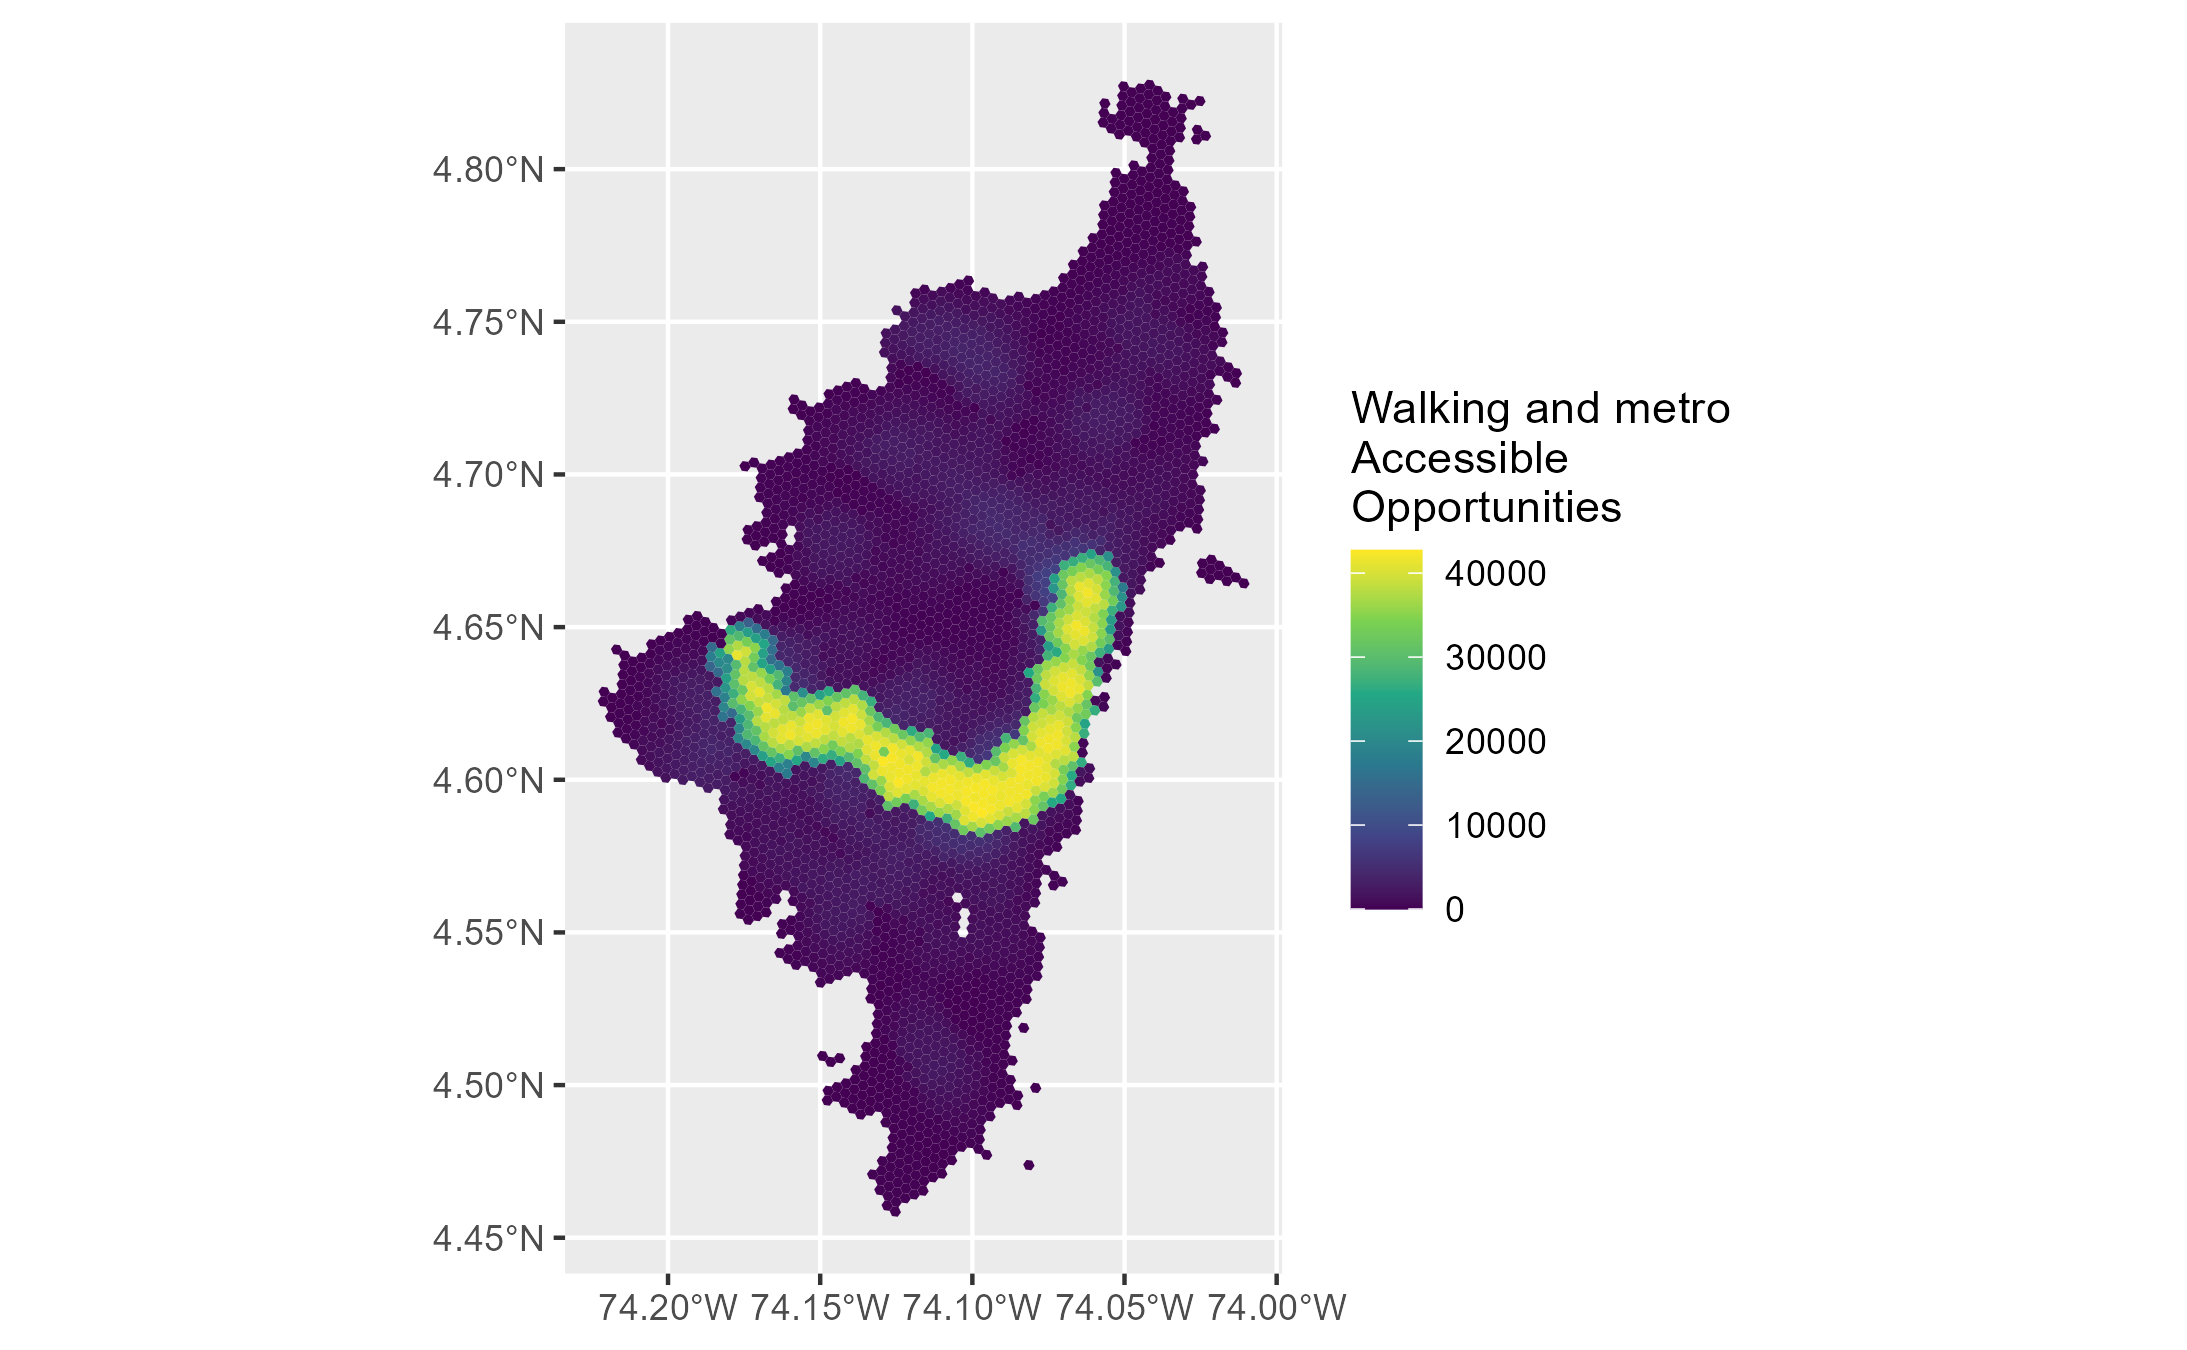
\includegraphics[width=1.3\linewidth]{Data/Results/Images/Access_Metro_base.png}
%         \caption{Metro}
%         \label{fig:Results_Walking}
%     \end{minipage}
    
%     \centering
%     \begin{minipage}{0.45\textwidth}
%         \centering
%         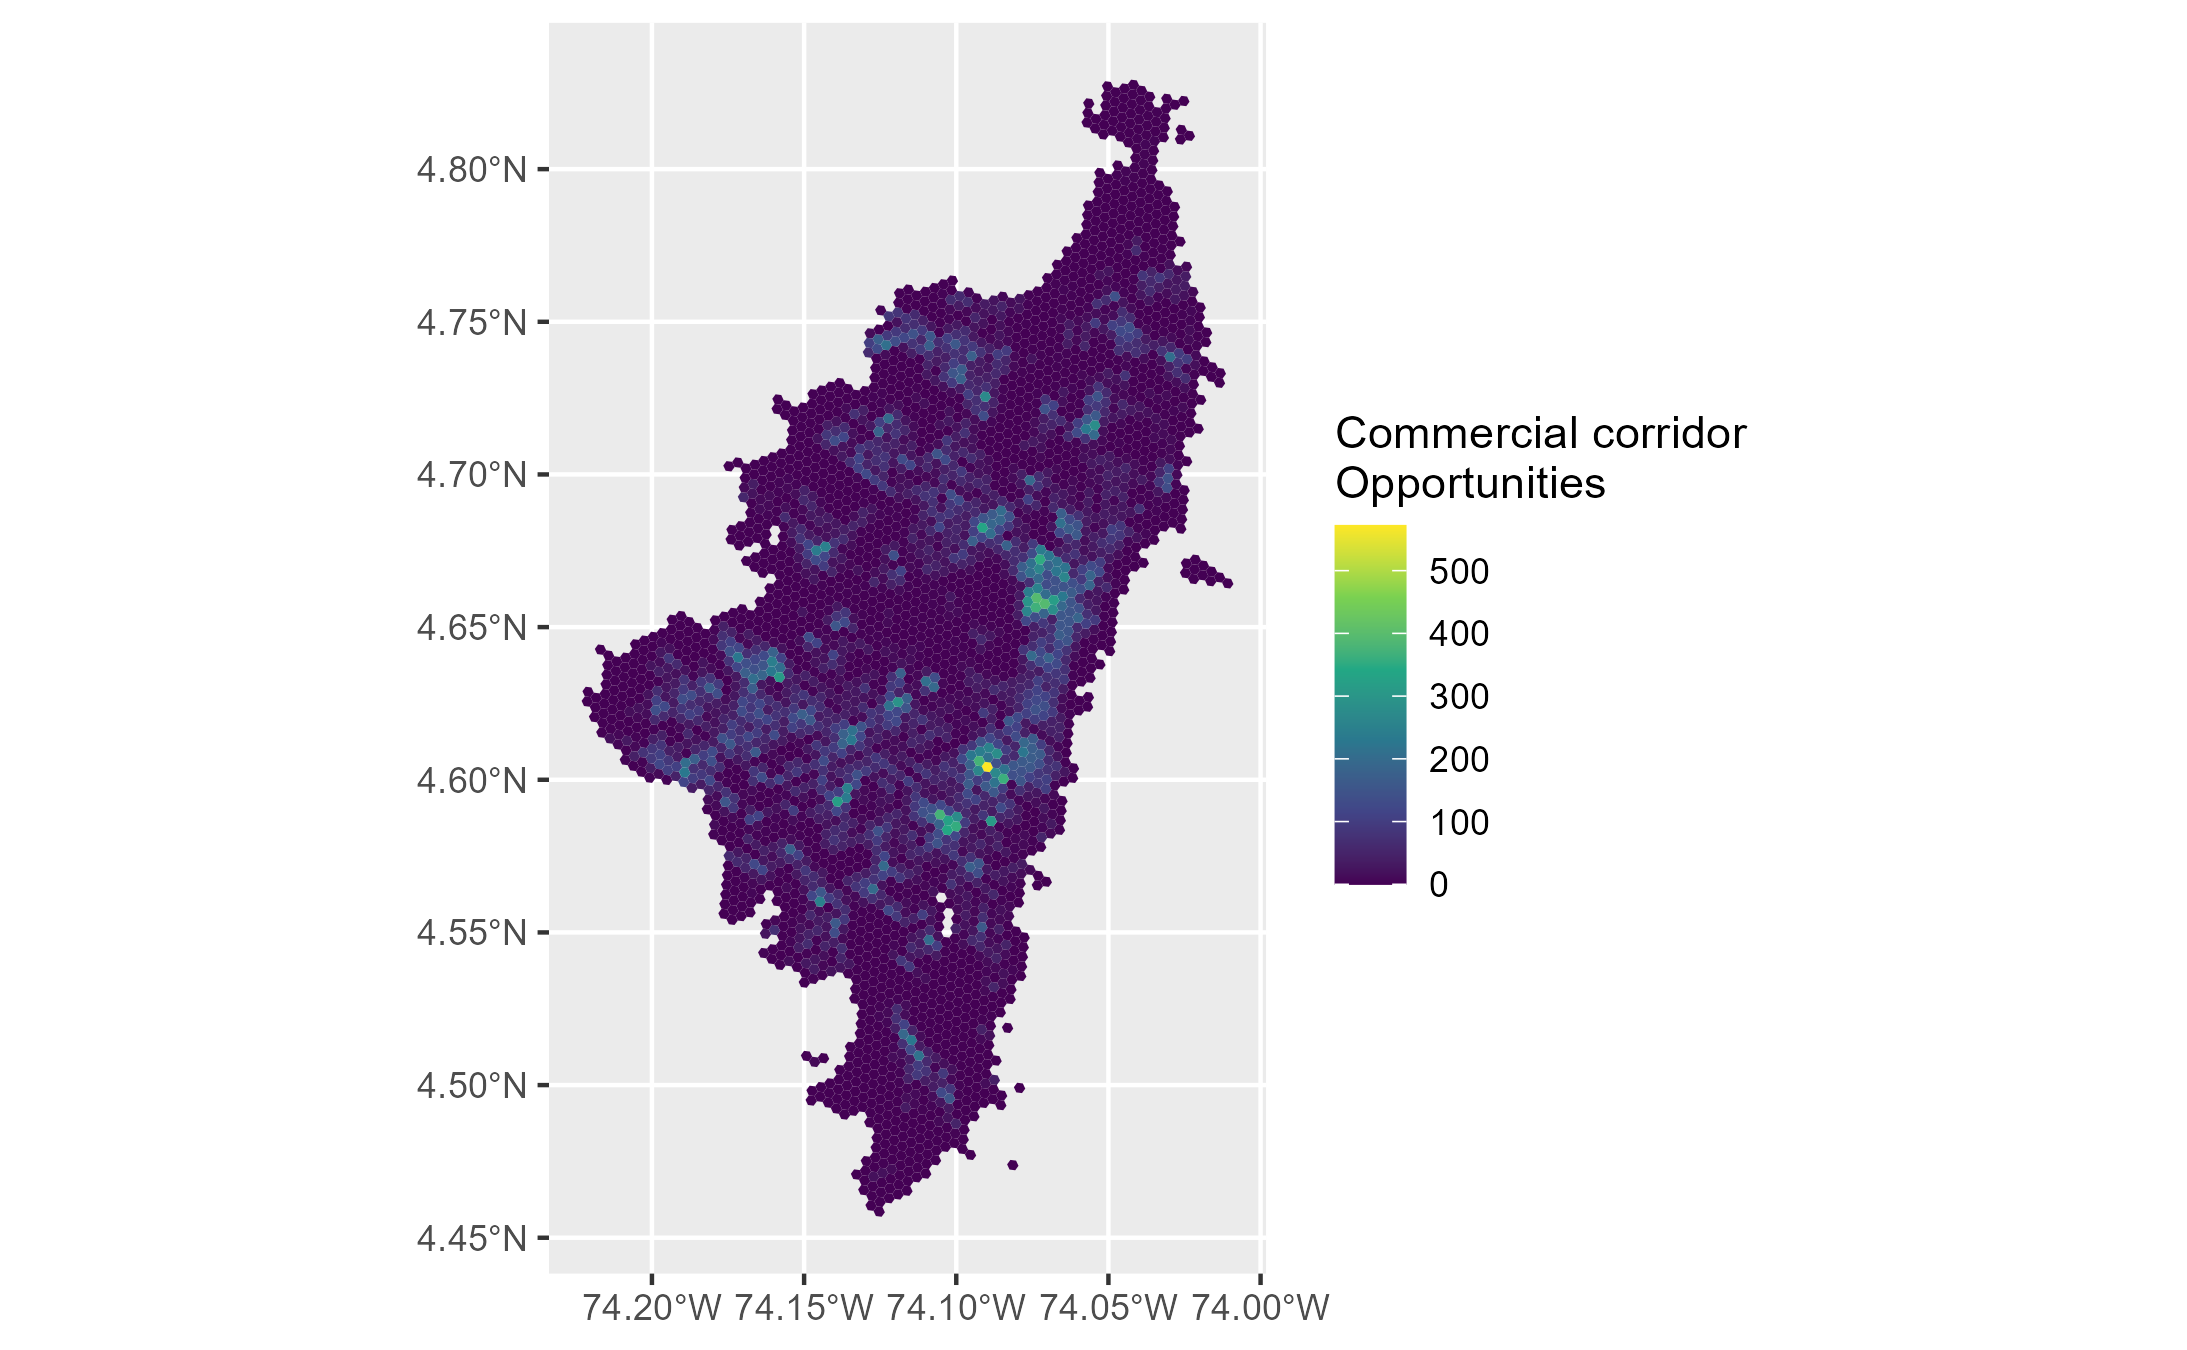
\includegraphics[width=1.3\linewidth]{Data/Results/Images/Opportunities_COD_21.png}
%          \caption{BRT and metro}
%         \label{fig:Results_Opportunities}
%     \end{minipage}
% \end{figure}

\begin{figure}[H]
    \centering
    \begin{minipage}{0.45\textwidth}
        \centering
        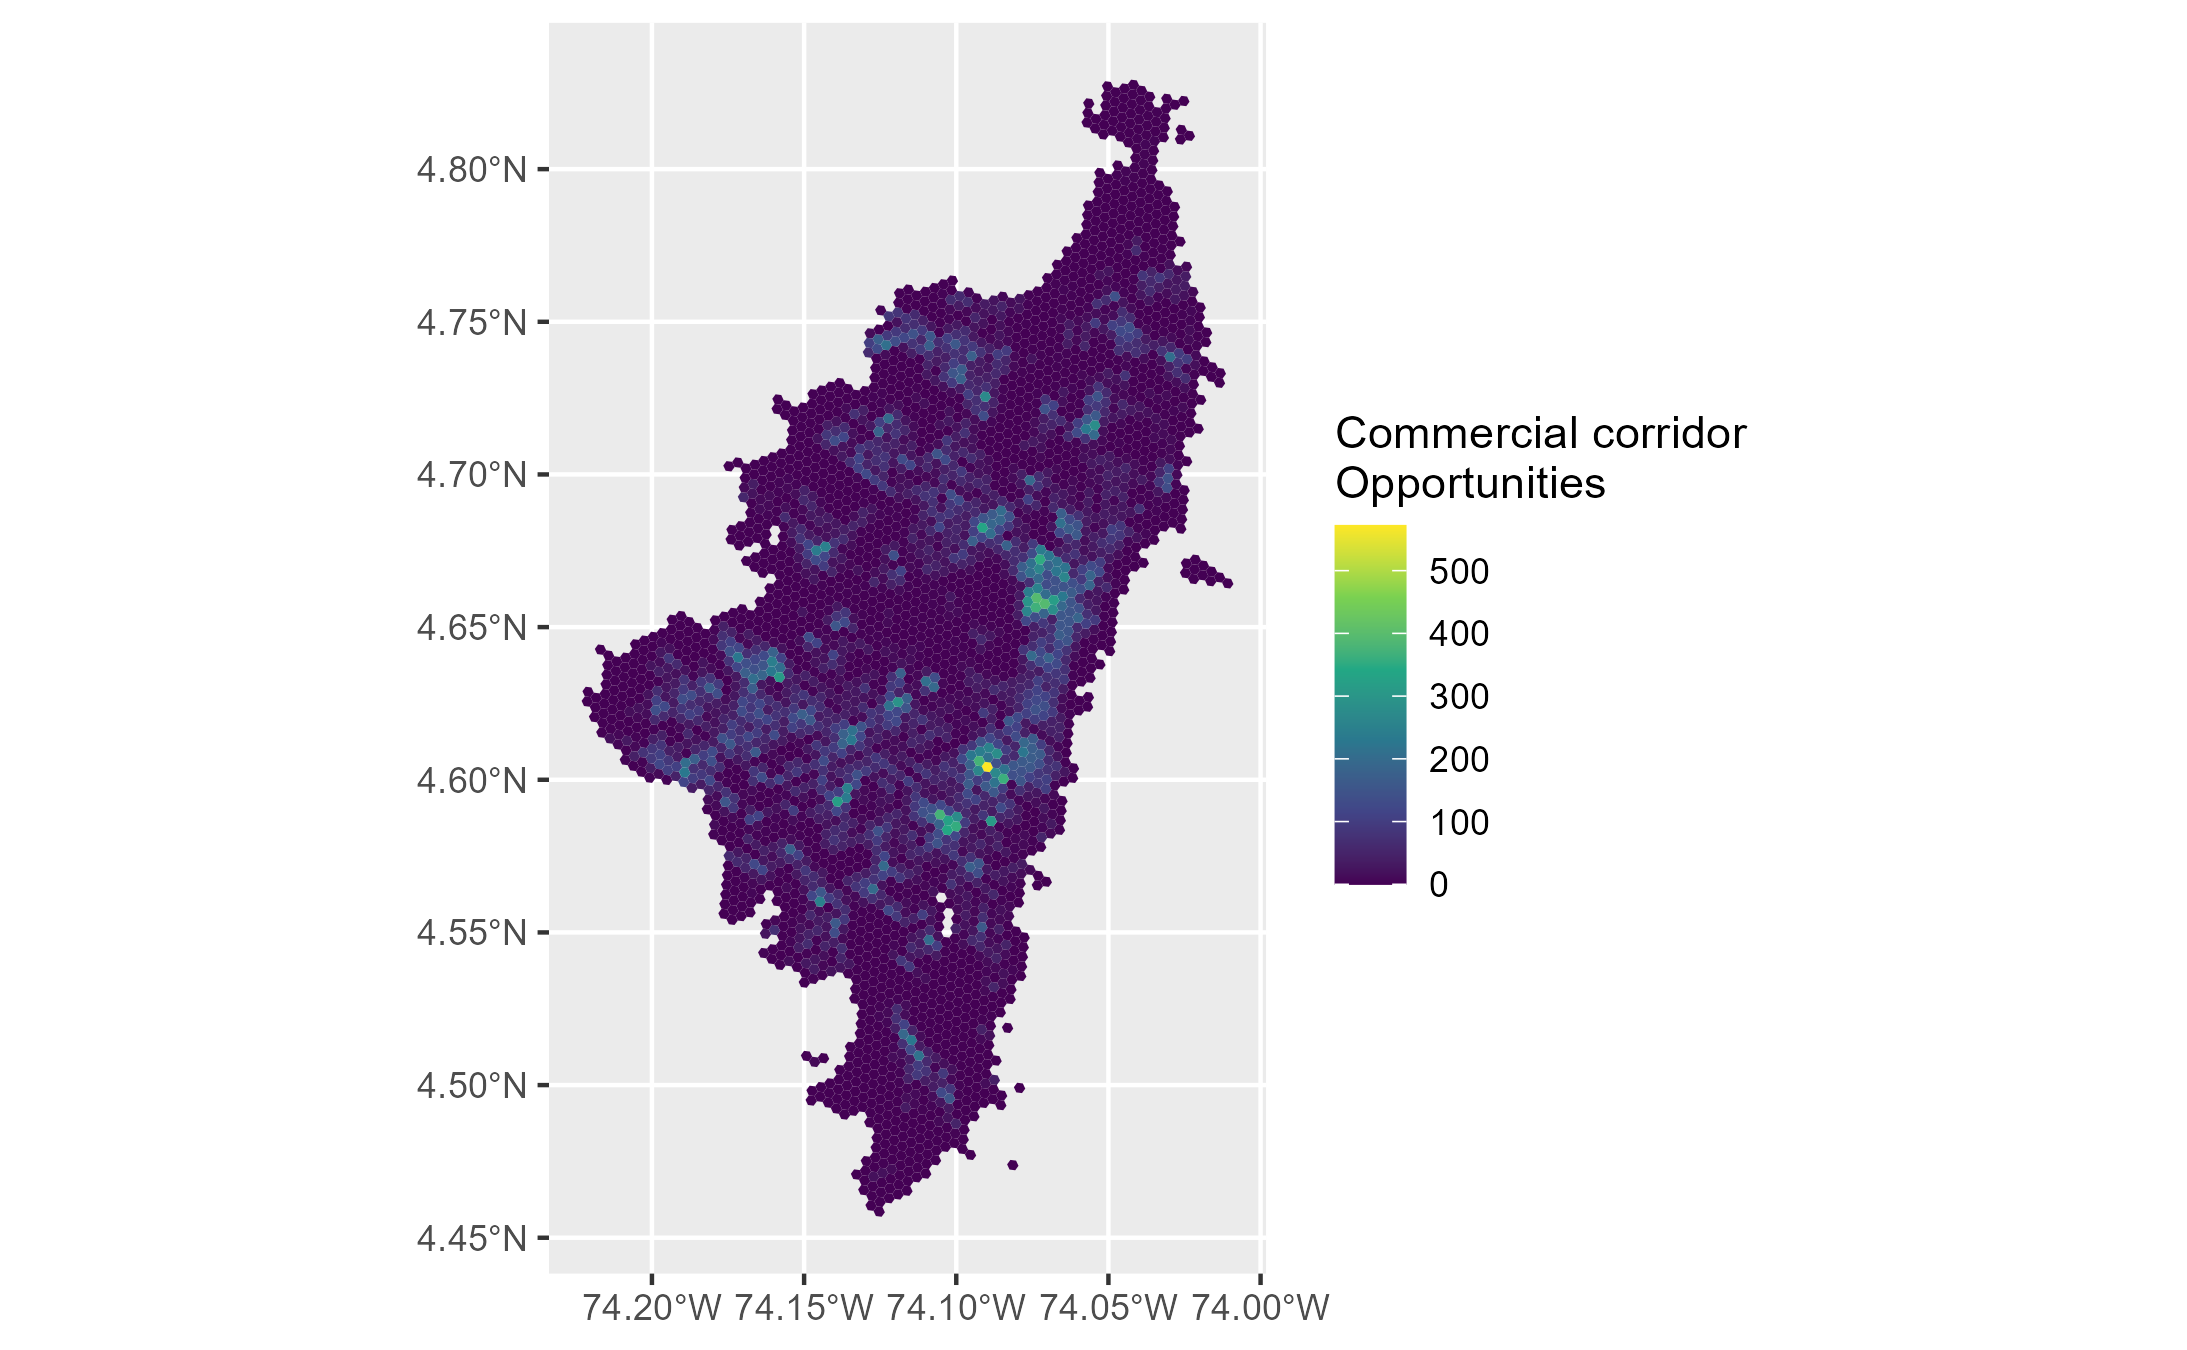
\includegraphics[width=1.3\linewidth]{Data/Results/Images/Opportunities_COD_21.png}
         \caption{Opportunities}
        \label{fig:Results_Opportunities}
    \end{minipage}%
    \hfill
    \begin{minipage}{0.45\textwidth}
        \centering
        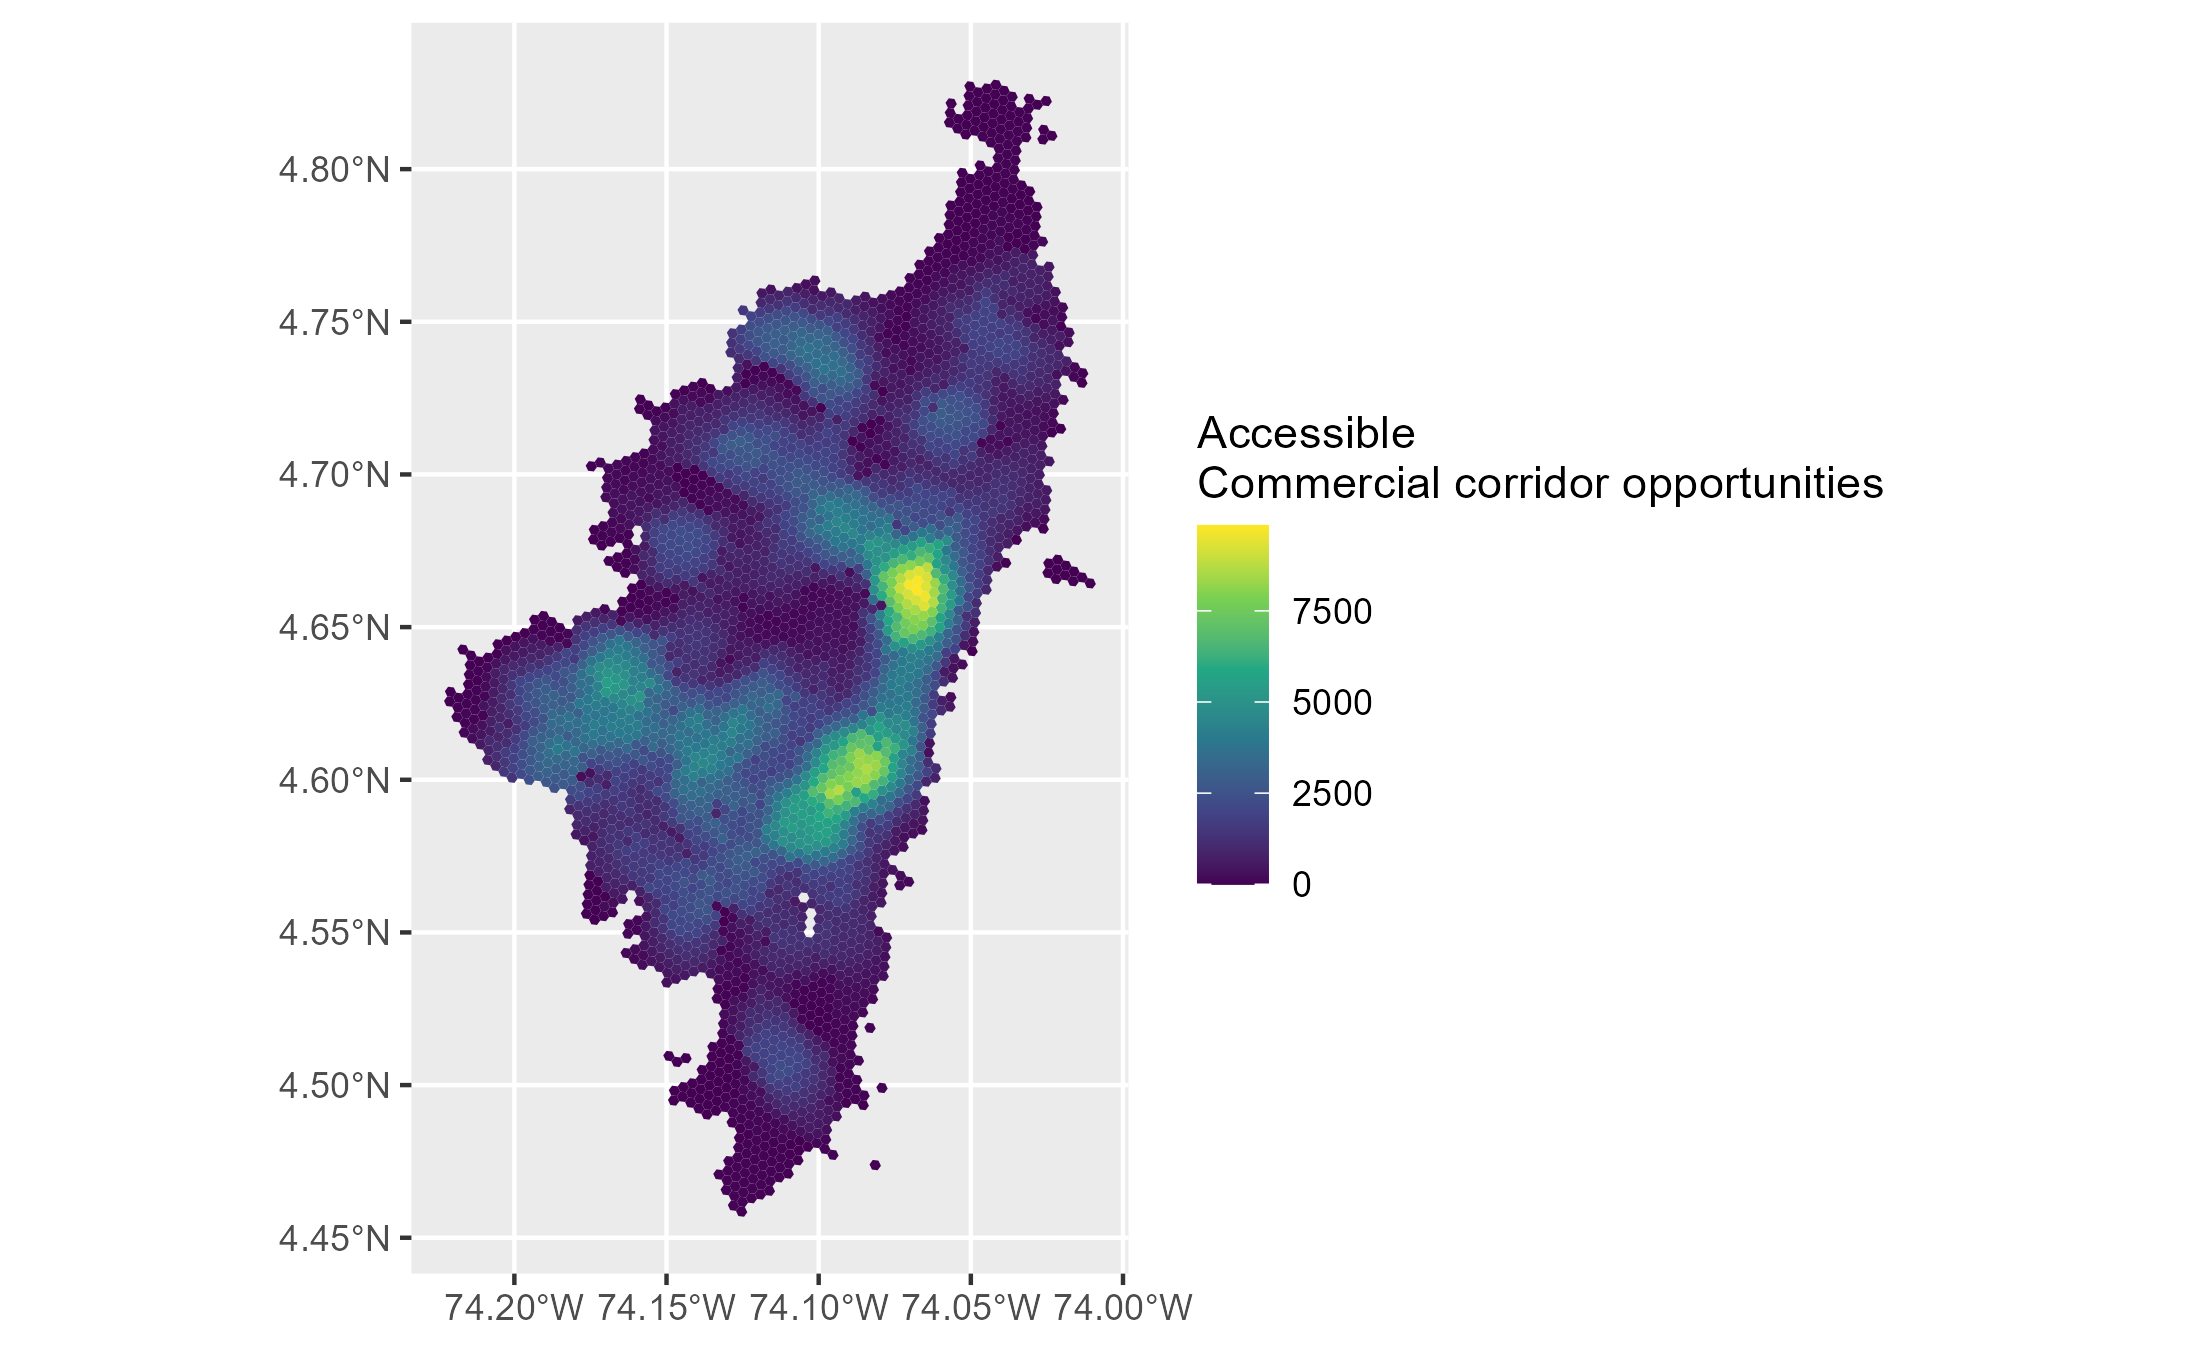
\includegraphics[width=1.3\linewidth]{Data/Results/Images/Access_Walk_base.png}
        \caption{Walking}
        \label{fig:Results_Walking}
    \end{minipage}
\end{figure}

\begin{figure}[H]
    \centering
    \begin{minipage}{0.45\textwidth}
        \centering
        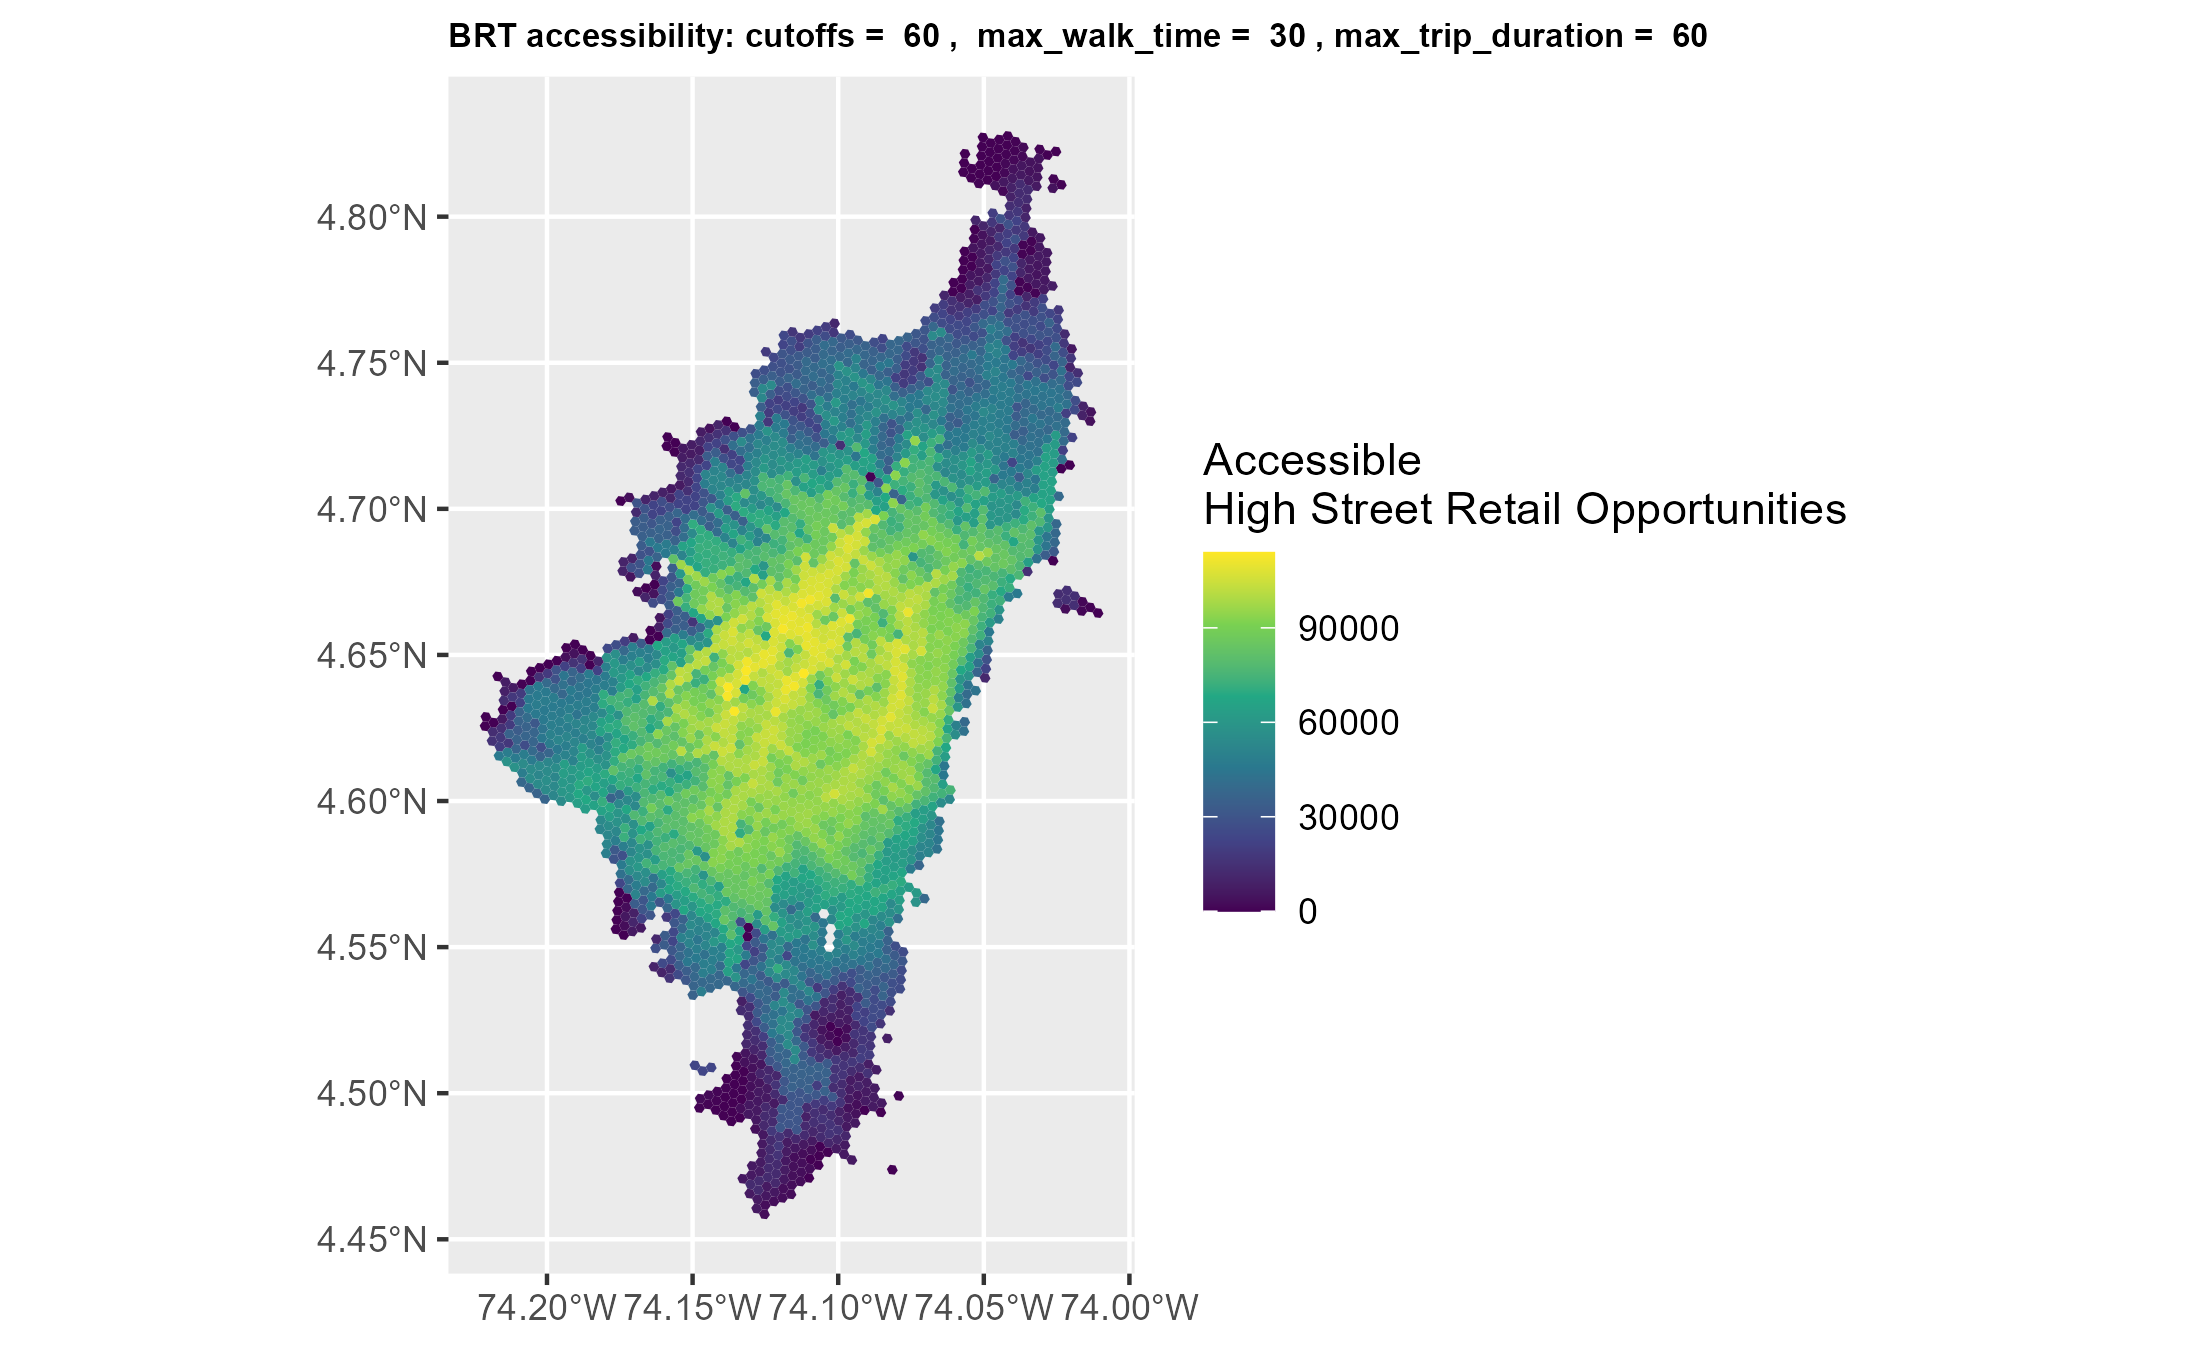
\includegraphics[width=1.3\linewidth]{Data/Results/Images/Access_BRT_base.png}
         \caption{BRT}
        \label{fig:Results_Opportunities}
    \end{minipage}%
    \hfill
    \begin{minipage}{0.45\textwidth}
        \centering
        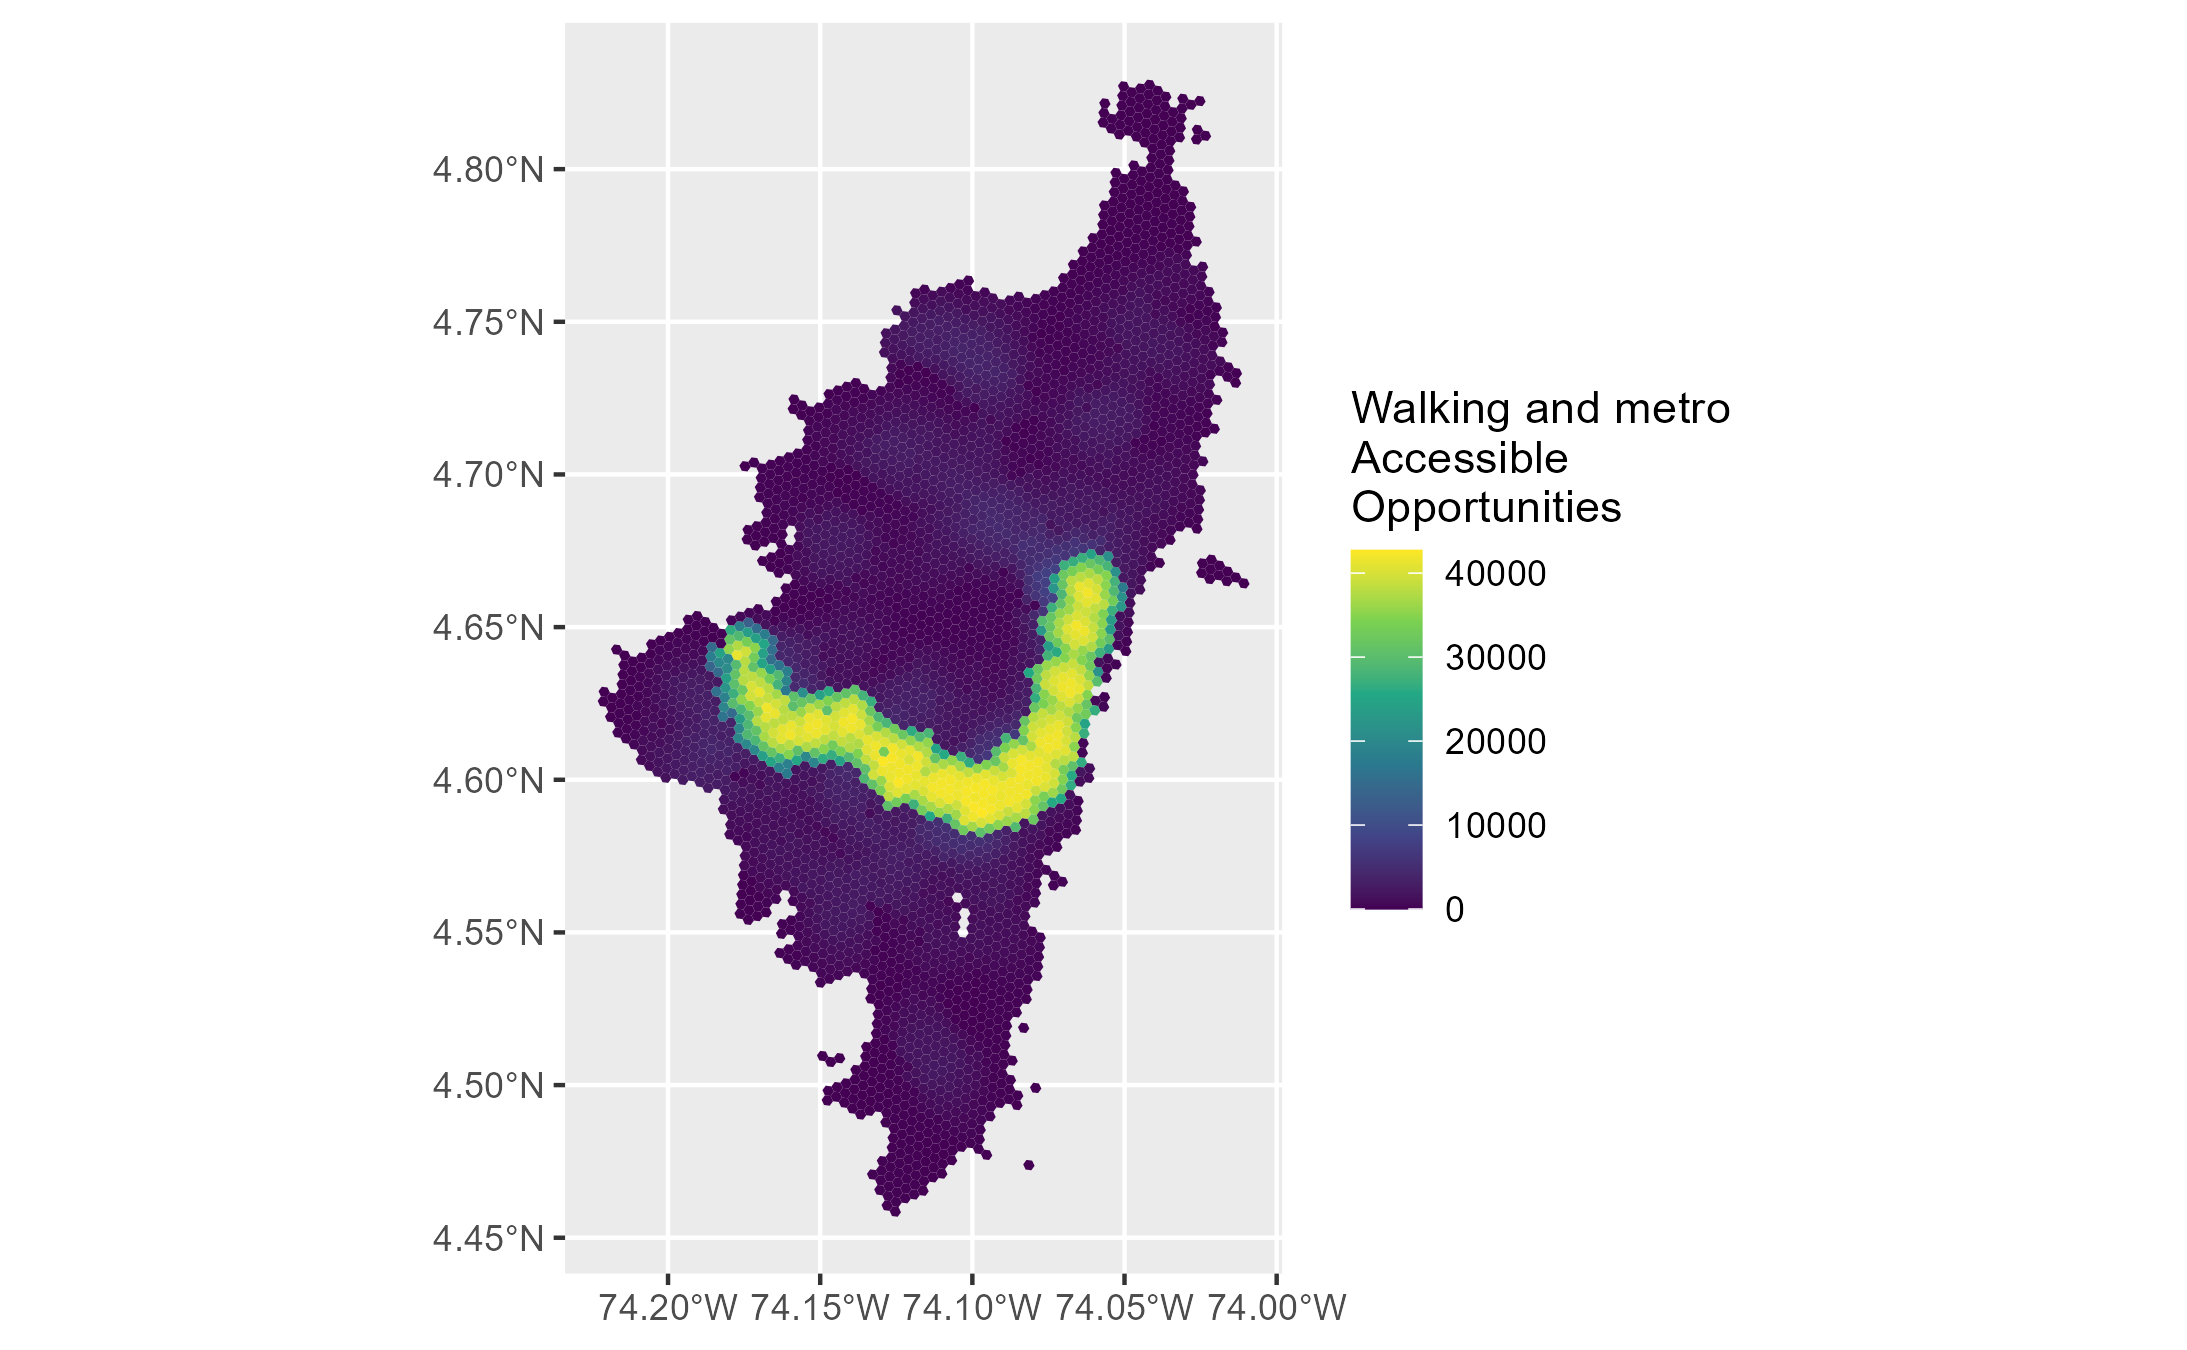
\includegraphics[width=1.3\linewidth]{Data/Results/Images/Access_Metro_base.png}
        \caption{Metro}
        \label{fig:Results_Walking}
    \end{minipage}
    \begin{minipage}{0.45\textwidth}
        \centering
        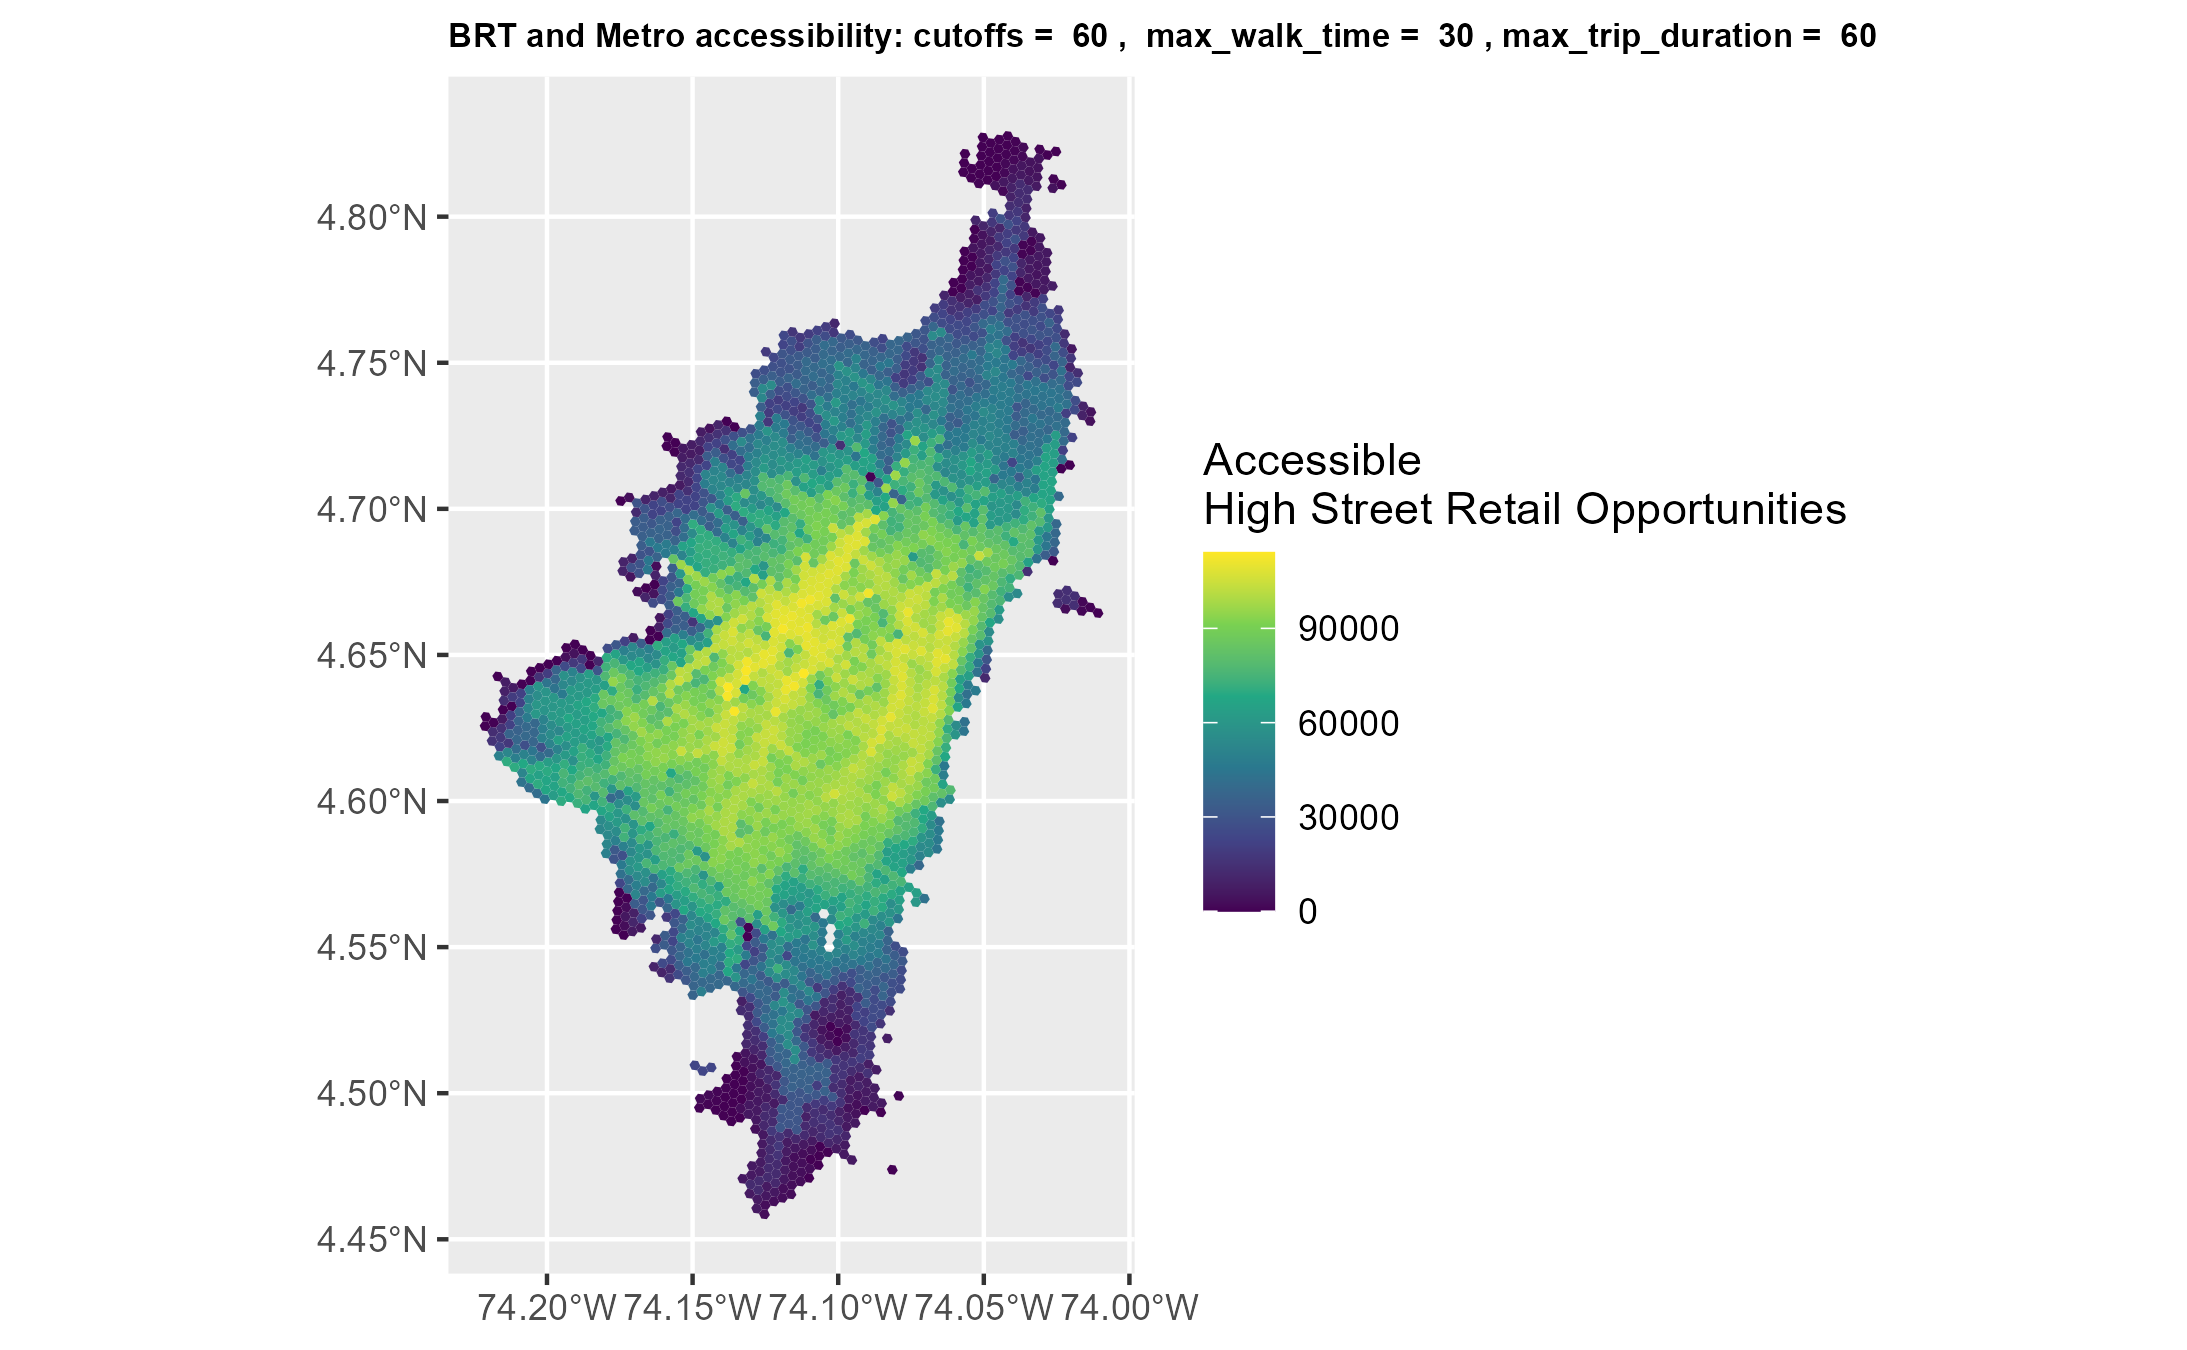
\includegraphics[width=1.3\linewidth]{Data/Results/Images/Access_BRT_Metro_base.png}
         \caption{BRT and metro}
        \label{fig:Results_Opportunities}
    \end{minipage}    
\end{figure}


\begin{figure}[H]
    \centering
    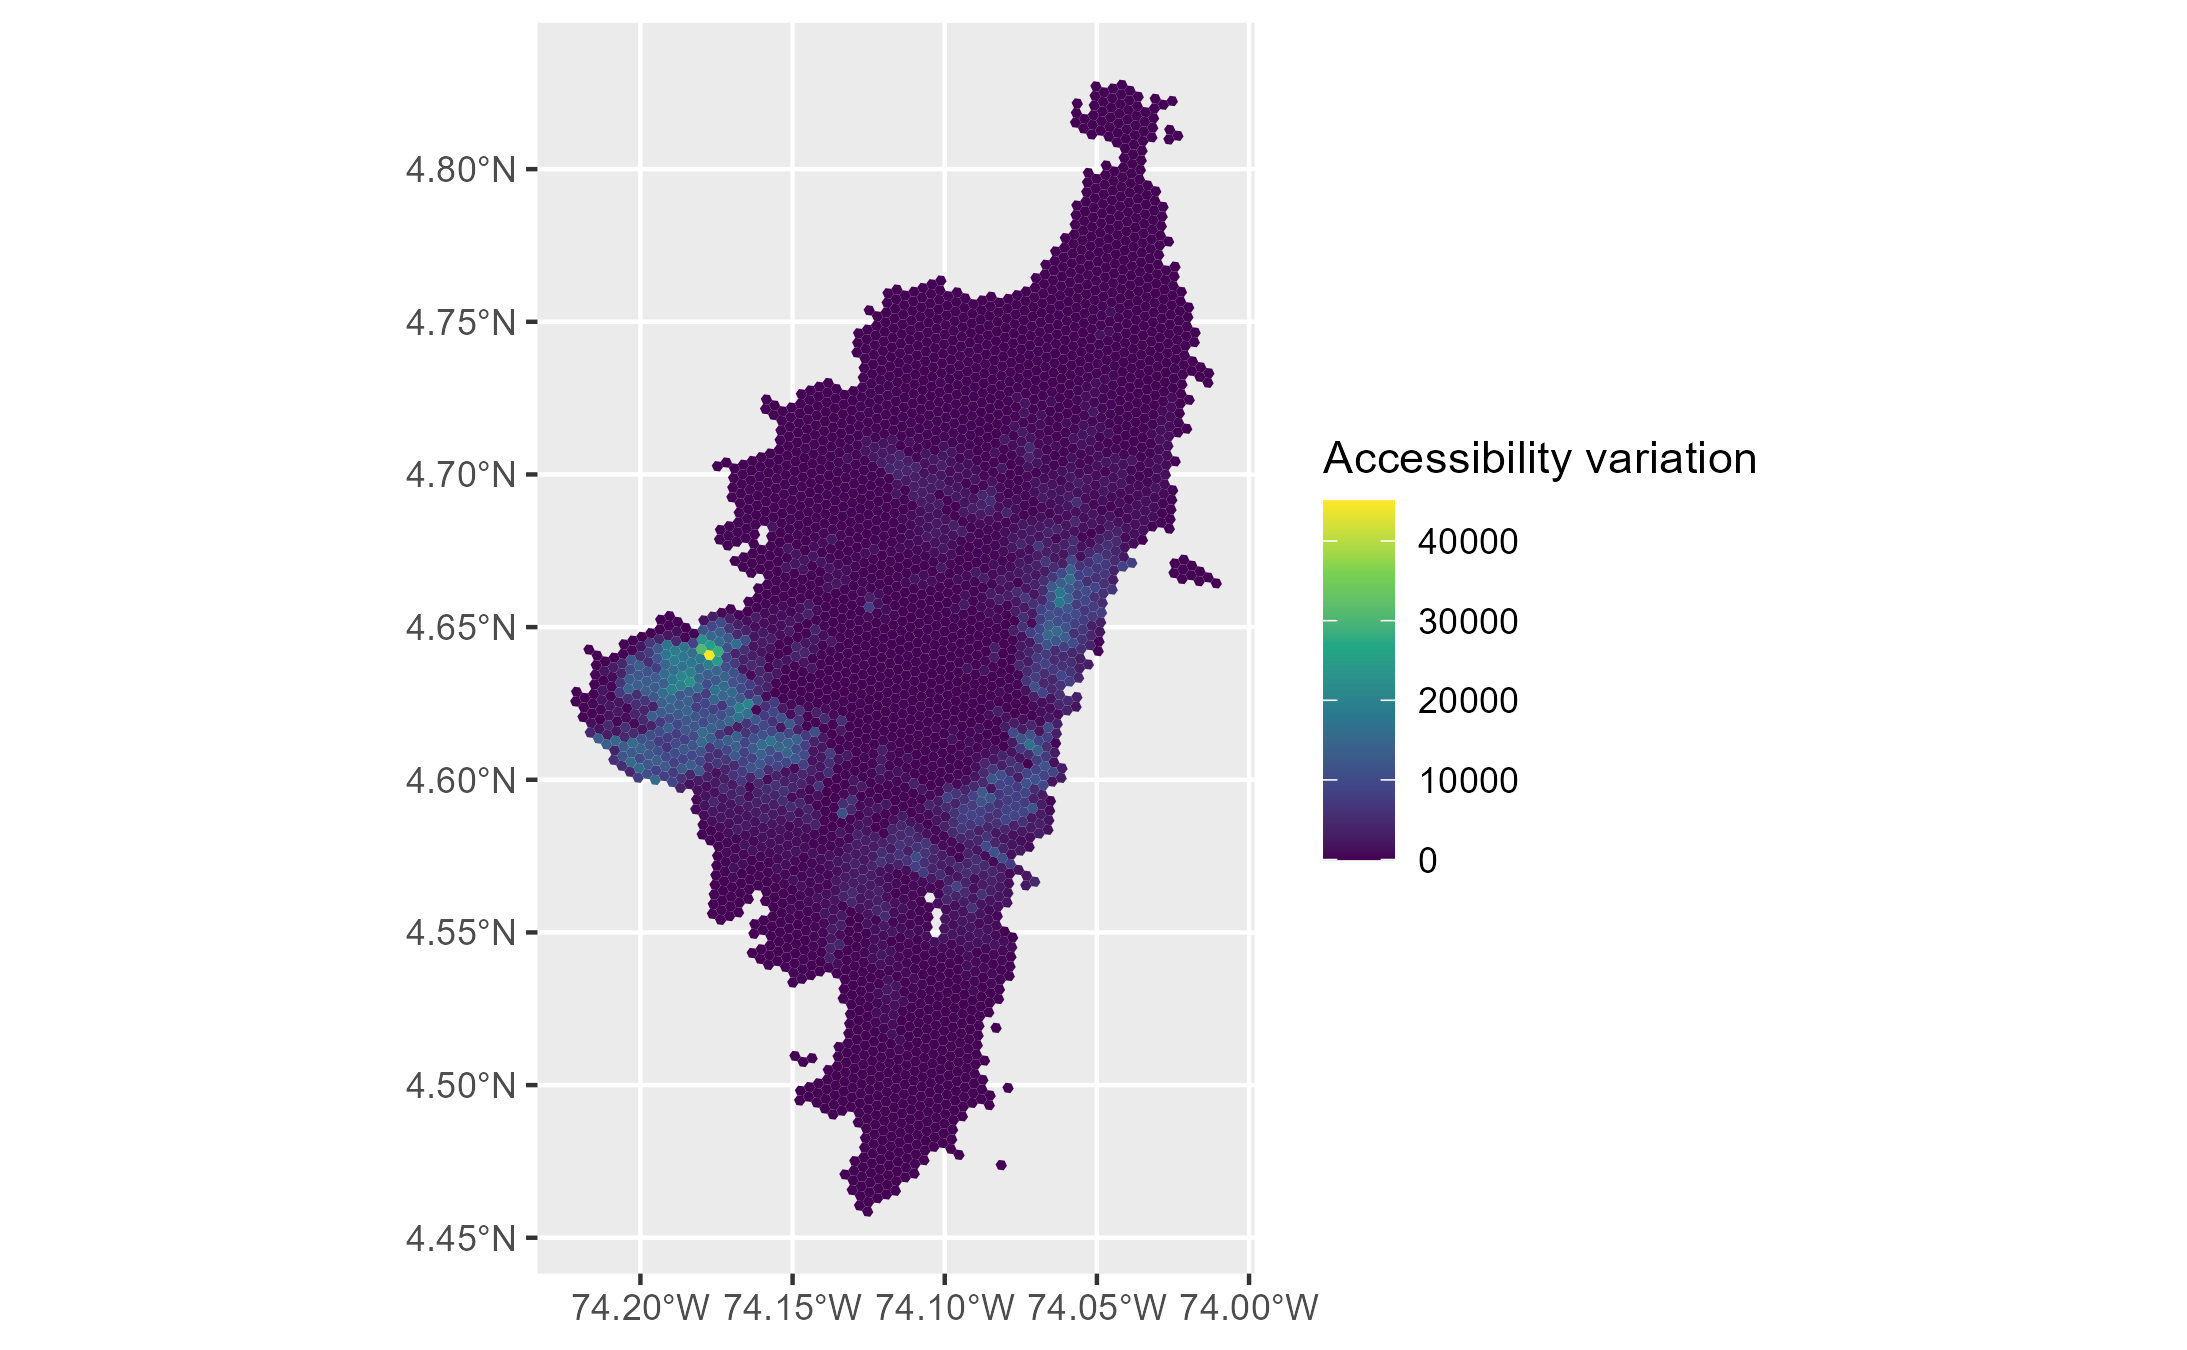
\includegraphics[width=14cm]{Data/Results/Images/Access_diff_BRT_Metro_base.png}
    \caption{Current and future scenario accessibility variation}
    \label{fig:Access_Variation}
\end{figure}


\section{Income groups}

\begin{figure}[H]
    \centering
    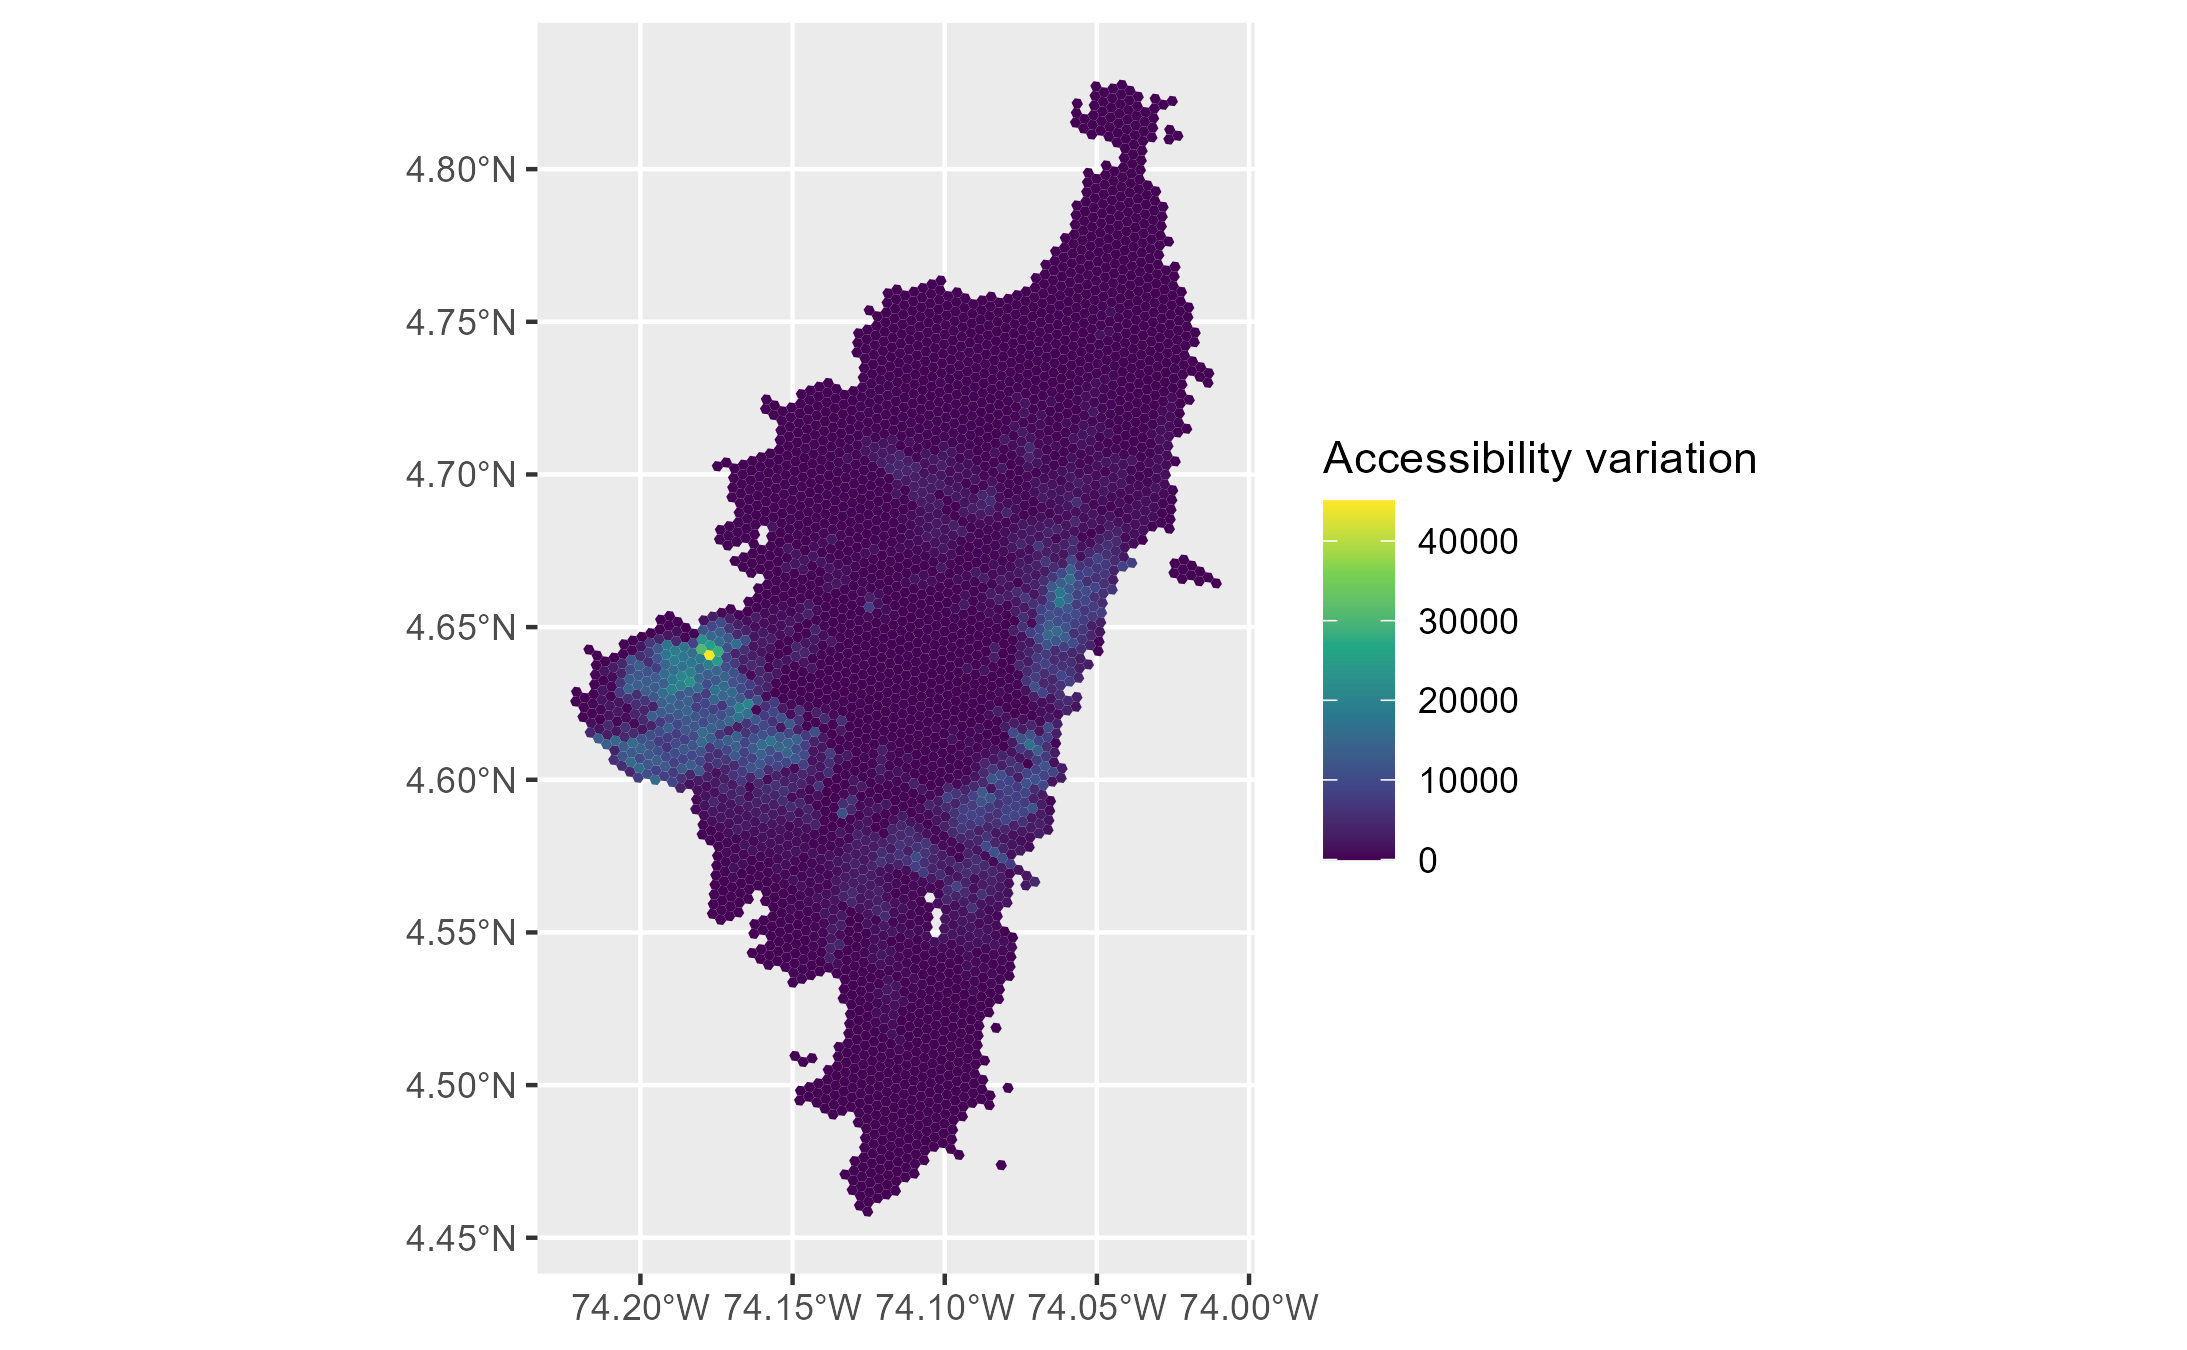
\includegraphics[width=14cm]{Data/Results/Images/Access_diff_BRT_Metro_base.png}
    \caption{Current and future scenario accessibility variation}
    \label{fig:Access_Variation}
\end{figure}

\chapter{Discussion} \label{Chap6}
\chapter{Conclusion} \label{Chap7}


\renewcommand{\bibname}{References}
\bibliographystyle{agsm}
%\bibliography{Bibliography.bib}
\bibliography{references.bib}
%%%%%%%%%%%%%%%%%%%%%%%%%%%%%%%%%%%%%%%%%%%%%%%%%%%%%%%%%%%%%%%%%%%%%%%%%%%%%%%%
% APPENDIX
\begin{appendices}
\chapter{Source code and data} \label{Source_Code}
Source code and data for all of the methods implemented in Chap. \ref{Chap4} for the project can be found in the remote repository: \href{https://github.com/rpoandres/MSc_USS_Dissertation}{GitHub}

% \chapter{Ethics review} \label{Ethics_Review}



% \chapter{Project Introduction Video}\label{sec:projectIntroduction}
% A short video presentation, introducing background, aims and organisation of the project, as of 30$^{th}$ June 2022: \newline
% \url{link}



\end{appendices}
%%%%%%%%%%%%%%%%%%%%%%%%%%%%%%%%%%%%%%%%%%%%%%%%%%%%%%%%%%%%%%%%%%%%%%%%%%%%%%%%
% GLOSSARY
\clearpage
\printglossaries

% INDEX?

\end{document}